\documentclass{report}

\usepackage{appendix}%for additional appendix options
\usepackage{float} %when using [H]: figure placed at exact spot
\usepackage{graphicx}
\usepackage{verbatim} % for multi-line comments
\usepackage{listings}
\usepackage{amsmath}
\usepackage[pict2e]{struktex}
\usepackage{parcolumns}
\usepackage{pstricks}
\usepackage{enumerate}% to be able to customize enumeration lists 
\usepackage[tight]{subfigure}%tight für weniger platz zwischen figures, see subfigrue docu
% \usepackage{multicol}
%\usepackage[rflt]{floatflt}

%\usepackage{fullpage}

%I've found the following lines in the internet to automatically begin a new line after a paragraph
\newcommand{\norm}[1]{\left|#1\right|}
\newcommand{\nnorm}[1]{\left|\left|#1\right|\right|}

\makeatletter
\renewcommand\paragraph{\@startsection{paragraph}{4}{\z@}%
  {-3.25ex\@plus -1ex \@minus -.2ex}%
  {1.5ex \@plus .2ex}%
  {\normalfont\normalsize\bfseries}}
\makeatother

%modification of page-margins
\addtolength{\hoffset}{-1.3cm}
\addtolength{\textwidth}{3.5cm}
%\addtolength{\textheight}{0cm}

%to change section numbering depth to 3 (default 2)
\setcounter{secnumdepth}{3}

%to change depth for appearence in table of contents to 3 (default 2)
\setcounter{tocdepth}{3}

\begin{document}

%% \documentclass[12pt]{article}

% \usepackage{ngerman}
% \selectlanguage{ngerman}
% \usepackage[latin1]{inputenc}

% \usepackage{graphicx}

% \begin{document}

\pagestyle{empty}

\begin{center}

\vspace*{-2.8cm}
\begin{minipage}[c]{.30\textwidth}
  \begin{flushleft}
    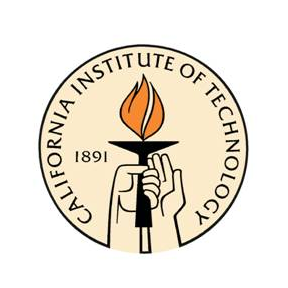
\includegraphics[width=3cm,clip=]{LOGO/caltech_logo}%
  \end{flushleft}
\end{minipage}
\begin{minipage}[c]{.43\textwidth}
\vspace*{1em}
    {GALCIT (Caltech)\\Prof. Hans G. Hornung \\ \\ Institute of Aerodynamics (TUM) \\ Prof.~Dr.-Ing. N.~A.~Adams}%
\end{minipage}
\begin{minipage}[c]{.25\textwidth}
  \begin{flushright}
    \vspace*{1em}
    
\includegraphics[width=3cm,clip=]{LOGO/TUMLogo_oZ_Vollfl_blau_RGB}%
  \end{flushright}
\end{minipage}

\vspace*{3.3cm}
\begin{minipage}[c]{11cm}
{\LARGE\bf 
Simuation of high enthalpy flow in porosities using SPH}
\end{minipage}

\vspace*{0.8cm}
Oliver Oberinger\\

\vspace*{2.8cm}
{\bfseries Diplomarbeit}

\vspace*{1.2cm}
%\large
\normalsize
\vfill
\begin{tabular}{ll}
Betreuer: & ~Prof. Hans G. Hornung (Caltech)\\
\ & \ Dipl.-Ing. Sergey Litvinov (TUM)\\
 \\
Ausgabe: & 15.\ Juni 2010\\
Abgabe: & 15.\ Dezember 2010\\
\end{tabular}

\vspace*{1.6cm}
%\large
Institute of Aerodynamics Technische Universit\"{a}t M\"{u}nchen\\
Graduate Aerospace Laboratories California Institute of Technology\\
2010	
\end{center}

\pagebreak
\pagestyle{plain}

%\end{document}


% \documentclass[12pt]{article}

% \usepackage{ngerman}
% \selectlanguage{ngerman}
% \usepackage[latin1]{inputenc}

% \usepackage{graphicx}

% \begin{document}

\pagestyle{empty}

\begin{center}

\vspace*{-2.8cm}
\begin{minipage}[c]{.30\textwidth}
  \begin{flushleft}
    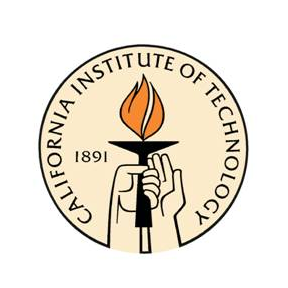
\includegraphics[width=3cm,clip=]{LOGO/caltech_logo}%
  \end{flushleft}
\end{minipage}
\begin{minipage}[c]{.43\textwidth}
\vspace*{1em}
    {GALCIT (Caltech)\\Prof. Hans G. Hornung \\ \\ Institute of Aerodynamics (TUM) \\ Prof.~Dr.-Ing. N.~A.~Adams}%
\end{minipage}
\begin{minipage}[c]{.25\textwidth}
  \begin{flushright}
    \vspace*{1em}
    
\includegraphics[width=3cm,clip=]{LOGO/TUMLogo_oZ_Vollfl_blau_RGB}%
  \end{flushright}
\end{minipage}

\vspace*{3.3cm}
\begin{minipage}[c]{11cm}
{\LARGE\bf 
Simulation of high enthalpy flow in porosities using SPH}
\end{minipage}




\vspace*{1.0cm}

Oliver Oberinger\\
\vspace*{1.0cm}
{\bfseries Intermediate version of Master's Thesis}\\
\vspace*{0.5cm}
for presentation at \\
\vspace*{0.3cm}
Institut Sup\'{e}rieur de l'A\'{e}ronautique et de l'Espace\\


\begin{minipage}[c]{.25\textwidth}
	
\includegraphics[width=3cm,clip=]{LOGO/LogoISAE}\\
\end{minipage}
\\
\vspace*{0.1cm}
responsible at ISAE: J\'{e}r\'{e}mie Gressier (Professeur SUPAERO)





\vspace*{1.2cm}
%\large
\normalsize
\vfill
\begin{tabular}{ll}
Advisors: & ~Prof. Hans G. Hornung (Caltech)\\
\ & \ Dipl.-Ing. Sergey Litvinov (TUM)\\
\ & \ Prof. Dr.-Ing. Nikolaus A. Adams (TUM)\\
 \\
\end{tabular}

\vspace*{1.6cm}
%\large
Institute of Aerodynamics Technische Universit\"{a}t M\"{u}nchen\\
Graduate Aerospace Laboratories California Institute of Technology\\
2010	
\end{center}

\pagebreak
\pagestyle{plain}

%\end{document}




\tableofcontents
\chapter{Introduction}
\label{sec:intro}


This work aims at the numerical simulation of high enthalpy flow over a porous
surface. The subject is of interest, as experiments CITATION
NEEDED (Prof. Hornung) have shown that wall porosity can damp
acoustic instabilities in hypersonic flows over a slender cone. A numerical
simulation of this configuration is desired to furnish data for a detailed
analysis of the active mechanism. The simulation method of choice for the first approach
to this configuration is called Smoothed Particle Hydrodynamics (SPH). 

SPH designates a meshfree method for numerical simulation of particle
ensembles (respectively matter that can be modelled as an ensemble of
particles as is the case for fluids).
Thus, the term particle ensemble not only refers
to fluids (as the name of the method would suggest) but also to solids. In
fact, nowadays, SPH is employed to simulate problems in different fields,
such as elasticity and fracture of solids, liquid flows and gas
dynamics~\cite{Monaghan2005}.
The initial developement of the method dates back to 1977, when Gingold and
Monaghan ~\cite{Gingold1977} tempted to compute an astrophysical gas dynamics problem with a new, compared to grid based methods more efficient approach. Independently and simultaneously, work in this field was also carried out by Lucy who came up with the same idea~\cite{Lucy1977}. One main advantage of SPH, which also is the reason why SPH was applied first to astrophysical problems, lies in the fact that it is a particle method and therefore does not need any room-fixed grid for the underlying numerical scheme. Instead
the base for the calculation of derivatives are discrete points, the particles, which move with the fluid (Lagrangian approach). Dealing with high density variations and huge calculation domains, astrophysical problems, when simulated with grid-based methods, 
required a considerable effort in terms of mesh-refinemend. For particle methods like SPH whereas, density variations are principally resolved naturally by a more or less dense particle spacing and calculation is only performed at places where there is matter, i.e. particles.
Another advantage is the relative ease of the
implementation of boundaries. And this is the main reason for the application of SPH in this work, as the structure of the solid boundaries represents a significant part of the problem, when treating porosities. 
 
%OTHER APPROACHES FOR CAVITY/POROSITY SIMULATION (look up in literature)
To be able to perform the simulation, a 2D compressible SPH code was developped in several stages and then validated by means of various test cases.
The first code that emerged from this project was a simple 1D compressible SPH code simulating a shock--tube problem. Although this code has no real use for practical applications, it is presented in this thesis with the goal to introduce the reader, who would like to familiarize himself with the implementation of SPH, to this technique.

The 2D code is based on an incompressible multi-phase SPH code, which was developed by \cite{Hu2006} and is now in use at the Institute of Aerodynamics of the TUM. This code was adapted in several steps to the needs of the present work, the first step being the implementation of the equations used in the 1D SPH code mentioned above and the adaption of the code to treat inviscid compressible problems. At this stage the code was tested for accuracy and robustness
by means of the 1D shock--tube problem. Both a 1D and a 2D particle distribution have been employed to this 1D problem. To conclude the 1D shock--tube tests, a study on the influence of perturbations in the particle distribution has been conducted, again both for 1D and 2D particle distributions.
At the same point, the simulation of acoustic wave propagation has been assessed, as acoustic phenomena are essential for the final flow configuration to investigate (see above).
In a next step the code was further adapted to incorporate physical viscosity and heat conduction models. The correctness of the implemented viscosity model was tested by analyzing the temporal decay of vortices using the Taylor--Green flow and the thermal conduction model was validated with a standard problem of pure heat conduction.
The final test--case, which is a compressibe Courrant flow with hot-- and cold--wall boundary conditions, combined all of the previously implemented models. It demonstrated that the combination of all the models would work with the required accuracy.
Finally, after the systematic validation of the code as an ensemble and of all its models separately, the actual configuration of interest, the flow through porosities, is simulated. 

The structure of this document is based on the classical structure of a scientific paper \cite{Day2006}, with the four chapters Introduction, Methods, Results and Discussio/Conclusion. If, when looking at the table of contents, the detailed organization of this document does not appear logical to the reader, the following lines are intended to point out the idea behind it.
In a first section, the Methods-chapter briefly describes the theoretical idea behind the SPH-method. The second section deals with some essential components of an SPH-implementation, followed by a section generally introducing the test-case problems and giving their analytical solutions, where possible. The general presentation of the test cases figures at this spot, as it is needed in the following sections. The next two sections explain the developed SPH-codes and also describe how to run them. Finally, there is a section describing the detailed simulation setup and post-processing procedure for each test-case, so that every result presented in this document may be exactly reproduced with the information given in this section.
RESULTS...



\chapter{Method}
\label{sec:method}
\section{Basic Idea of SPH}
\label{sec:BasicsSPH}

To illustrate the basic idea of SPH, it is helpful to first consider the
governing equations of fluid dynamics for an inviscid flow, the Euler equations. Remark: As SPH has its origin in Astrophysics, and as many astrophysical problems can be modeled by the Euler equations \cite{Liu2003}, it is these equations, on which the SPH formalism is based. 

%\begin {equation}
%Euler IN LAGRANGIAN FORM
%\end {equation}

%The above equations have the form~\cite{Monaghan2005}
The Euler equations have the form~\cite{Monaghan2005}

\begin {equation}
\label{eq:EFD_form}
{\frac{dA(r)}{dt}}=f(A(r),\nabla A(r),r)
\end {equation}
where
\begin {equation}
{\frac{d(.)}{dt}}={\frac{\partial(.)}{ \partial t}}+v\nabla(.)
\end{equation}
is the substantial derivative.

Thus the rate of change of  physical quantity depends on its spatial
derivatives. The goal of any method for numerical simulation is to approximate
these derivatives by information of a discrete number of points in order for a
computer to be able to handle it. 

The SPH method is based on the idea of approximating a function $A(x)$ by an
integral interpolant
\begin{equation}
\label{eq:int_interpolant}
A_I({\bf r})=\int A({\bf r'})W({\bf r}-{\bf r'},h)d{\bf r'}
\end{equation}

%\begin{equation}
%A({\bf r})=\int A({\bf r'})\delta({\bf r}-{\bf r'})d{\bf r'},
%\end{equation}

where $W({\bf r}-{\bf r'},h)$ is the so called kernel or smoothing function and $h$ the
smoothing length. If $W$ is the delta function this interpolation is exact,
otherwise it represents an approximation. As the theoretically
perfect kernel, the delta function, is of no practical use, the kernels
employed in practice are functions which tend to the delta function in the 
limit $h\rightarrow 0$.
Examples for those kernel functions are a Gaussian kernel or
kernels based on Schoenbergs~\cite{Schoenberg1946} $M_n$ splines~\cite{Monaghan2005}.
More details on kernels are given in section
(\ref{sec:KernelFunction}) and in the book on SPH published by Liu~\cite{Liu2003}.

The fact of using a kernel different from the delta function constitutes the
first of two approximations made by the SPH
method. It is often referred to as {\bf kernel approximation}~\cite{Liu2003}.
The second approximation consists of a discretization of the integral
expression in equation~(\ref{eq:int_interpolant}), thus changing the integration
to a summation over all discretized elements of the domain - the particles. 
This allows for the determination of $A_I(\bf{r})$ by numerical methods. In the SPH
literature, this second approximation is commonly called {\bf particle
approximation}~\cite{Liu2003}.

With the relation between mass, density and volume for each discretized particle
\begin{equation}
m_i=\rho_i V_i,
\end{equation}
applying the particle approximation to equation (\ref{eq:int_interpolant}) leads to the following expression:

\begin{equation}
\label{eq:intInter}
A_S({\bf r})=\sum_b m_b \frac{A_b}{\rho_b}W({\bf r}-{\bf r}_b,h).
\end{equation}


In the same way, the derivative of the field function $frac{dA(x)}{dx}$ can be
approximated to give~\cite{Monaghan2005} or \cite{Liu2003} 
%(in Liu with gradient,im Monaghan for 1 direction)

\begin{equation}
\label{eq:simpleDerivative}
\nabla A_S({\bf r})=\sum_b m_b \frac{A_b}{\rho_b}\nabla W({\bf r}-{\bf r_b},h).
\end{equation}

The disadvantage of the above equation (\ref{eq:simpleDerivative}) is, that for
$A(\bf{r})=const.$ the approximated derivative does not vanish. By writing 
%(in Monaghan the equation figures not with gradient but only in 1 direction!?!)
\begin{equation}
\label{eq:derivativeIdentity}
\nabla A = \frac{1}{\Phi}(\nabla {\Phi A}-A\nabla \Phi),
\end{equation}
where $\Phi$ is any differentiable function, this problem can be resolved. In its
SPH form  equation (\ref{eq:derivativeIdentity}) reads as follows:

\begin{equation}
\nabla_a A = \frac{1}{\Phi_a}\sum_b \frac{m_b}{\rho_b}(A_b-A_a)\nabla_a W_{ab}.
\end{equation}

It can be seen that the approximation to the derivative of the
field function $A$ is now expressed by a summation over the field function itself
and the derivative of the kernel function - which can be determined exactly.

Now the basic SPH formulations are introduced: both the field function
itself and its spatial derivatives can be approximated using only information 
of a discrete number of particles. Hence, the rates of change of
the states described by the Euler equations of fluid dynamics, which are of the form
corresponding to equation (\ref{eq:EFD_form}), can be rewritten using this information. Thus 
one obtains the SPH formulation of the equations of fluid dynamics.

The detailed derivation of the SPH equations for fluid dynamics will not be shown here, as the
interest  only lies in describing the principle ideas behind the SPH
method. To summarize, these are as follows: a fied-function can be
described as an integral interpolation over the function itself and a kernel
function, which has to be chosen in an appropriate way (c.f. section (\ref{sec:KernelFunction})). A further
approximation consists in transforming the integral over the domain into a
summation over the discrete elements - the particles - constituing this domain. 
This allows to express both
the field function and its spatial derivatives in a form  
that depends exclusively on discrete values
of the field function itself (and of the kernel function and its derivatives, 
all of which are known). By finally choosing an appropriate kernel function $W$ with
compact support, i.e. a finite support domain, where $W=0$ beyond, the summation over all particles in the calculation domain can be reduced
to a summation over those particles within the support domain of the particle
in question.

%Übergang zu diesem Abschnitt gefällt mir noch nicht, v.A siehe Beginn voriger Abschnittt
The SPH formulation of the equations of fluid
dynamics is obtained by applying the above principles and conducting different
transformations to the original differential equations. Depending on the
transformations used, the final SPH equations can assume a different form. In
the following, a common form for the rates of change of density, velocity and
internal energy based on the Euler equations, i.e. without viscosity and heat conduction, is listed \cite{Monaghan2005,Liu2003}: 
%(perhaps also list NSG-form, and
%explain why Euler is of interest as well (for 1DSPH code, perhaps later real
%code including viscosity???)

\begin{equation}
\label{eq:DCR_Euler}
\frac{d\rho _a}{\mathit{dt}}=\sum_b{m_{b}{\bf v_{\mathit{ab}}}\nabla _{a}W_{\mathit{ab}}},
\end{equation}

\begin{equation}
\label{eq:VCR_Euler}
\frac{ d {\bf v_{a}}}{\mathit{dt}}=-\sum_b {m_{b}\left(\frac{P_{a}}{\rho_{a}^{2}}+\frac{P_{b}}{\rho _{b}^{2}}\right)\nabla_{a}W_{ab}},
\end{equation}


\begin{equation}
\label{eq:ECR_Euler}
\frac{de_{a}}{\mathit{dt}}=-\mathit{}\frac{1}{2}\sum_b{m_{b}\left(\frac{P_{a}}{\rho _{a}^{2}}+\frac{P_{b}}{\rho _{b}^{2}}\right){\bf v_{\mathit{ab}}}\cdot\nabla _{a}W_{\mathit{ab}}}.
\end{equation}

For the detailed derivation and for alternative formulations of
these equations refer to \cite{Monaghan2005, Liu2003}.



%\section{Implementation of an SPH code}
\section{Features of an SPH code}
\label{sec:FeaturesOfSPH}
This section presents some features of a generic SPH code and different variants of these features. Emphasis is
placed on these variants that will finally be implemented in one of the
two SPH codes designed and modified during this work.
Points of interest are a closer description of the kernel function, different methods to perform the search for the interacting particles, as well as the implementation of different boundary conditions in
SPH. Furthermore, different
equations of state are introduced, depending on the nature of the flow problem
to be considered (compressible/incompressible), followed by a passage
explaining the need of artificial viscosity. The challenges of implementing a physical viscosity model and a heat conduction model are highlighted thereafter. Subsequently, some numerical
integration schemes that have proven to be reliable for SPH applications are discussed and the two different possibilities to calculate the density are shown. Finally a general structure of a generic SPH code is given.

Note: in this section the above mentionned features are discussed in a general perspective, independent of the particular implementation in a concrete code. The latter will be done in section (\ref{sec:CompAndStruc1DCode}) for the 1D code and in sections (\ref{sec:Comp2DCode}) and (\ref{sec:Struc2DCode}) for the 2D code which gives a more complete view.




\subsection{Kernel function}
\label{sec:KernelFunction}
% ???not sure, if its the right place here, but somewhere there should be a
% paragraph with more detailed information on kernels used, compact support,
% perhaps even some properties,...(and perhaps some graphics???)


Some properties of kernel functions, also called smoothing functions, and notions related
to them have already been mentionned in section
(\ref{sec:BasicsSPH}). In principle, every function can act as kernel function
if it respects a set of criteria listed by~\cite{Liu2003}.
The most important ones are (list not exhaustive):
\begin{itemize}
\item The smoothing function should vanish outside of a certain area around its
center. This property, which is expressed in equation (\ref{eq:compactSupport}, is called compact support and the domain where $W\neq0$
is the {\bf support domain} of the smoothing function. The {\bf support length} $\kappa h$ and the
{\bf smoothing length} $h$ are not to be confused.
 
\begin{equation}
\label{eq:compactSupport}
W(x-x')=0,\textit{for}|x-x'|>\kappa h
\end{equation}

\item The smoothing function should be normalized to 1, which ensures that constants
are interpolated exactly:
\begin{equation}
\int{W(x-x',h)dx'}=1.
\end{equation}

\item The smoothing function should tend towards the delta function as the smoothing
length $h$ tends to zero:
\begin{equation}
\lim\limits_{h \rightarrow 0}{W(x-x',h)}=\delta(x-x').
\end{equation}
This is to ensure consistency of the integral approximation, which means that
the approximate expression tends to the exact expression of the integral
interpolant equation for $h \rightarrow 0$.
\end{itemize}
The above list does not contain all necessary SPH kernel properties. Its complete version can be found in  \cite{Liu2003}.
Based on those properties a variety of kernels are used in SPH literature. A
very commonly used kernel is the $M_4$ kernel (cubic spline) based on Schoenberg's
$M_n$-Splines~\cite{Schoenberg1946}.

\begin{equation}
\label{eq:cubicSpline}
M_{4}(x)=\begin{cases}
\frac{1}{6}[(2-q)^{3}-4(1-q)^{3}],& \text{for 0 $\leq$ q $\leq$ 1} \\
\frac{1}{6}(2-q)^{3},&  \text{for 1 $\leq$ q $\leq$ 2} \\
O,& \text{for q $>$ 2}.
\end{cases}
\end{equation}


In the work of \cite{Fulk1996} a measure of merit for kernels is developed and
they came to the result that, at least in 1D, no kernel performes significantly better
than the cubic spline.
This is why for the 1D SPH code described in section (\ref{sec:1DSPHcode}) the cubic spline kernel was employed.

The unit of the kernel function $W$ is the inverse of the volume or the corresponding 1D/2D equivalent, as can be seen easily from equation (\ref{eq:SumDensity}) which is only introduced below.


\subsection{Neighboring particle search methods}
\label{sec:NNPS}
To calculate the derivatives in equations (\ref{eq:DCR_Euler})-(\ref{eq:ECR_Euler}), principally a
summation over all particles has to be performed. However, as we defined kernel
functions $W$ with a compact support, i.e. $W=0$ beyond a certain distance from the particle in question, only particles within this distance, the so called support length (see section (\ref{sec:KernelFunction})), contribute to the
interpolation of the origin particle's values, and thus interact with it. Finding the interacting
particles is one of the key features in an SPH implementation, as an effective
interaction search method, often also called {\bf nearest neighboring particle (NNP)
search} method in the SPH literature, can considerably reduce
computation time. 

The most basic NNP algorithm is called {\bf all pair search}, and as its name
suggests all imaginable particle pairs are tested for interaction. This means
that the calculation process consists of a double loop where the outer loop
iterates over all particles and defines one of the pair's partners (often
refered to as origin). For each of the (origin) particles an inner loop is
performed, which iterates again over all particles thus defining the other
partner (destination) of the pair. Then, the pair is tested for the
interaction condition, meaning that their distance has to be smaller than the
support length. In this way, for a calculation domain consisting of $N$
particles, $N*N$ iteration steps and tests have to be executed. The
calculation cost of this approach is $O(N^2)$. 
If the
interactions are assumed to occur pairwise, i.e. if there is a spatially constant
smoothing--, and therefore support--length,
%THINK ABOUT THE AVERAGED SMOOTHING LENGTH...)
there is a simple but efficient way of reducing computation
time. Thus, if a pair $P_{ij}$ is an interaction, the pair
$P_{ji}$ is an interaction as well. That way half of the $O(N^2)$ iterations
and tests can be eliminated, leading to a complexity of $O(N!)$. 
%(LOOK FORREFERENCES). 
This approach is employed in the 1D SPH code as it is easy to
implement\cite{Liu2003} and the number of particles in this 1D simulation is
still reasonably low in order not to have to use more sophisticated algorithms
such as are introduced below.
\\
A more effective but also more complicated method is the {\bf linked list
algorithm}. This is based on the fact that kernels with compact support are
used and thus interacting particles may only be located in the neighborhood of
the particle under consideration. The computation domain is divided into cells with
cell size $\ge \kappa h$, ideally $=\kappa h$, and the
particles are assigned to the cell they are located in~\cite{Monaghan1983}. In this way the cell
structure serves as a book--keeping device and in case of an interaction
calculation with an origin particle $i$ not all the particles $j,j={1,...,N}$ have
to be considered but only those particles in the adjoining cells. Hence, the
complexity of the original problem which is of order $O(N^2)$ can be reduced
considerably and even tends to $O(N)$ if the particles in one cell are few. 
%FIGURE: DIAGRAM WITH CELLS /PARTICLES /DOMAIN!?!
Technically the cells are managed by the implementation of a linked list
structure in a computational code. More details on this are given in section
(\ref{sec:2DSPHcode}), as this algorithm is implemented in the 2D
SPH code, and besides in \cite{Monaghan1985, Hockney1988}.

However, the method has a drawback if used with a spatially variable smoothing
length. In this case the cell size is not ideally adapted to every particle
and the algorithm looses efficiency.
\\
Moreover, different other NPP techniques exist which, here, shall not be introduced in
detail. One class of these are called {\bf tree search algorithms}~\cite{Hernquist1989}, which are
especially robust and efficient for problems with variable smoothing
length~\cite{Liu2003}.
% and therefore are implemented in many astrophysical applications, as h=variable essential due to the huge variation of quantities













\subsection{Boundary condition implementation}
\label{sec:boundaryConditionImplementation}
For particles at the edge of the calculation domain, the summation interpolation does not
give exact results, as the integral (or better the sum) is truncated due to
the simple fact that outside the domain there are no
particles~\cite{Liu2003}. (find better citation...) This effect is called the
the particle deficiency
problem.\cite{Liu2003}. In cases where the region of interest is far from boundaries
and where information from the domain edges does not propagate to the region of interest
in the time of interest, there is no need to consider this
problem. 
The 1D shock tube simulation with 1D particle distribution described further below
(PERHAPS LINK TO SECTION)is an example of such a case.  

But for many applications precise boundary conditions have to be applied and it is therefore necessary to treat the edges of the domain in a special manner, depending on the desired boundary condition. This often includes the placement of so--called virtual particles or ghost particles within the distance of one supportlength outside the domain, which are assigned properties according to the boundary condition to implement.
These virtual particles, that were originally used by \cite{Libersky1993}, then contribute to the calculation of the quantities of the real particles inside the domain. Thus the particle deficiency problem can be solved. 
 Following paragraphs which detail this and alternative concepts for the different types of boundary conditions

\paragraph{periodical boundary condition}
The periodical boundary condition is relatively easy to implement and consists of placing a copy of all real particles within one supportlength to one domain edge right in front of the opposite domain edge.



\paragraph{symmetrical boundary conditions}
A way of setting up symmetrical boundary conditions is mirroring all real particles within one supportlength to the domain edge at the latter.

\paragraph{solid--wall}
For solid wall conditions, beside the fact of avoiding the particle deficiency problem, a second issue is to prevent particle penetration into the wall.
There are two types of solid wall conditions: a free-slip condition, which is appropriate for inviscid flow, and a no--slip condition which has to be applyied for modelling solid walls in viscous flow simulations. The free-slip wall condition does essentially not differ from the symmetry condition, except for the case where thermal boundary conditions may be applied as well. While the symmetrical BC is by condtruction always adiabatic, the free-slip wall provides the possibility to implement an isothermal BC by fixing the boundary particle's temperature.

As wall boundary conditions in this project are mainly needed for viscous flow simulations, the no--slip condition is of special interest. In this case an additional issue is to reproduce this no--slip condition. A good overview on solid wall boundary implementations for (incompressible) viscous flows is given in \cite{Yildiz2009}. 
According to \cite{Yildiz2009} and personal research such no-slip solid walls are mainly applied for SPH-simulations of low Reynolds-number and for incompressible or weakly-compressible fluid--models. 

The problem of particles penetrating the solid walls can be adressed by either implementng a reflection law or a repulsive force at the boundary. Monaghan originally linked the repulsive force in a form similar to Leonard-Jones potential to boundary particles placed directly ON the boundary \cite{Monaghan1994} but this approach turned out to produce considerable perturbatios in the real particle movement paralell to walls \cite{Monaghan2005}. An improved approach by Monaghan uses a different force model \cite{Monaghan2004} that gives remedy to these perturbations. Due to the fact, that the boundary particles are placed exclusively on the boundary, an error in density due to the particle deficiency problem can still aoccurr and appropriate correction methods might be applied \cite{Monaghan2004}. Concerning the no--slip condition, Monaghan claims, that it can be achieved with his model by including the boundary particles, which have the velocity of the boundary, in the viscous force calculations. 

A different approach for modelling solid--walls consists in placing ghost particles outside the domain up to a distance of one supportlength to the boundary. The particle deficiency problem is therefore solved, but no explicit measure is taken to prevent particles from penetrating into the solid wall in case the ``normal'' interaction forces produced by the ghost particles are not sufficient.

 These methods differ in their complexity and efficiency 
\begin{enumerate}
  \item in the way the ghost particles are placed, and
\item in the way their velocities (or in general properties) are assigned to prevent particle penetration and ensure the no--slip condition.
 \end{enumerate}

Concerning the first point, different options are imaginable. Ghost particles can either be placed once during the simulation setup and then maintained (fixed to the wall they represent) for the entire simulation. Or they can be recreated every timestep by mirroring the positions of the corresponding real particles at the boundary. In the easiest case of a linear/plane boundary this corresponds to the ghost particle placement for periodical or symmetrical boundary conditions as mentionned above.
For more complex geometries however mirroring can only be applied with restrictions, so that a fixed ghost particle placement once at the beginning of the simualation, as done for example by \cite{Morris1997, Morris1999}, is more convenient. Only sophistcated approaches, such as \cite{Yildit2009} recreate ghost particles by mirroring for complex geometries at every timestep.

The easiest way of velocity assignment for ghost particles to obtain a no--slip condition is by simply immobilizing them relative to the boundary they are to represent \cite{Morris1997}, i.e. all ghost particles have the same velocity which is zero for a non-moving boundary or the corresponding boundary velocity for a boundary in motion.This gives a first order no--slip condition. A velocity assignment leading to a more accurate no--slip condition can be done by either mirroring or extrapolating the corresponding real particle profile. \cite{Basa2009} tested these different approaches in a poisseuille channel and found out that discrepancies with the exact solution mainly occurr right at the boundary during the initial phase.  According to these tests, mirroring of velocities is the least accurate method, followed by linear and then quadratic extrapolation. 

In combining these options one can reconstruct some boundary treatment approaches already mentionned in literature.
\begin{itemize}

 \item An approach where the ghost particles are created each timestep by mirroring the positions of the real particles is adopted in the 2D code for modelling of solid walls with no--slip or free--slip conditions at the edges of the computational domain.
The ghost particles have the same properties as their real counterparts
except for the velocity. Depending on the type of boundary condition they are
supposed to represent, different velocities are assigned to them \cite{Hu2006}.

No--slip velocity boundary condition:
\begin{equation}
v_{virtual}=2v_{wall}-v_{real}.
\end{equation}

Free slip velocity boundary condition:
\begin{equation}
v_{virtual}^{tangential}=v_{real}^{tangential}.
\end{equation}

FIGURE: ILLUSTRATION OF VELOCITY ASSIGNMENT FOR VIRTUAL BOUNDARY PARTICLES

\item The approach from Morris \cite{Morris1999} combines a fixed ghost particle positionning with an linearly interpolated velocity and is apllied in the original publication for modelling porosities in a low Reynolds-Number incompressible flow.
This way of modelling boundary conditions is implemented for the porosity representation within the calculation domain. 
To form a curved bondary, ghost particles are set up in layery parallel to the boundary with the first layer directly at the boundary. 
Note: for porosity representation this leads to the problem of filling the remaining space with real particles of constant density. Suggested solution \cite{Morris1997}: Placing regular lattice real particles in places where there are no porosities and first leting particle configuration relax before applying driving force! (or directly setup the porosity ghostparticles to gether with the real particles in a single regular lattice: leads to inaccurate curved surface representation for low resolutions \cite{Monaghan1997})

The velocity of the ghost particles is assigned according to the following principle:
blablabla!!!

\end{itemize}


As already indicated above, the ghost particle approach alone might not completely prevent a penetration of real particles into the boundary. For this reason \cite{Liu2002} has combined the boundary particle concept from Monaghan with the ghost particle concept by simultaneous use of both particle types.  NOTE: This approach can be kept in mind for the porosity implementation if it turns out that the pure ghost-particle appraoch leads to boundary penetration ENDNOTE


begin alter text:-------------------------------

 To address the second issue, different approaches have been conceived that include strong repulsive forces at the boundary.

conditions. This can be accomplished by a special boundary treatment which
often includes  The first ones to come up with this idea were
\cite{LIBERSKY1993}. Virtual particles are used to model solid walls by
placing them inside the solid body, mirrored at the surface. For each real
particle whose support domain interferes with the wall, one such particle is
built. Virtual particles have the same properties as their real counterpart
except for the velocity. Depending on the type of boundary condition they are
supposed to represent, different velocities are assigned to them.\cite{Hu2006}.

No--slip velocity boundary condition:

\begin{equation}
v_{virtual}=2v_{wall}-v_{real}.
\end{equation}

Free slip velocity boundary condition:

\begin{equation}
v_{virtual}^{tangential}=v_{real}^{tangential}.
\end{equation}

FIGURE: ILLUSTRATION OF VELOCITY ASSIGNMENT FOR VIRTUAL BOUNDARY PARTICLES

For the treatment of periodic boundary conditions, no ghost particles are
needed. Particles leaving the calculation domain on one side are simply
reinserted on the opposite side (with the same properties).

end alter text-------------------------------------------

\subsection{Equation of state}

The equation of state relates the pressure $p$ 
to the density $\rho$ and in general also the internal energy $e$, or equivalent.
An equation of state is needed for the solution of compressible flow problems, as the energy equation is not decoupled from the mass and momentum equation unlike for incompressibly treated flows: for the latter, the density $\rho$ is constant and therefore not a variable of the problem, leaving the pressure $p$ and the velocity vector $v$ as unknowns of the problem. These, in the general 3D case, four variables are faced by the four equations of mass and momentum conservation which makes the problem solvable. If the density becomes an unknown of the problem as well, further equations have to be consulted to solve the problem.
%%Was heißt denn Problem SCHLIEßEN???  
 
For the application of SPH to gas dynamics, the assumption of an ideal gas is often
appropriate.
%(citation and conditions). 
In this case the corresponding equation of state is

%...equation of state in the original form...

%...
%transformation steps (or at least realations needed)...

\begin{equation}
\label{eq:idealGasEqState}
 p=(\gamma-1)\rho e.
\end{equation}

The sound speed, which is needed to calculate the artificial viscosity (see equation (\ref{eq:FactArtVis})), can be formulated for an ideal gas as:

\begin{equation}
\label{eq:soundSpeed}
 c=\sqrt{\gamma R T}
\end{equation}
or, with $c_v T=e$, $R=c_p-c_v$ and $\gamma=\frac{c_p}{c_v}$,

\begin{equation}
 c=\sqrt{\gamma(\gamma-1)e}.
\end{equation}

Different equations of state need to be used in other media. For example, according to Monaghan~\cite{Monaghan1994,Monaghan2005}, even liquids, which are commonly approximated
as incompressible (such as water) are treated as weakly compressibly is SPH. This requires a corresponding equation of state. As this equation of state does not depend on the temperature though, the energy equation is decoupled from the rest of the equations and there is no need to solve it - exactly as it is known for the truly incompressible case.



\subsection{Artificial Viscosity}
\label{sec:ArtVisc}

Another point that has to be taken into account for SPH simulations, especially
if shock waves are present, is artificial viscosity \cite{Monaghan2005}. This
prevents particles from penetrating one into another in zones with high
compression rates and also generally stabilizes a numerical
algorithm.
Artificial viscosity for numerical simulations of shock phenomena
in general was first introduced by \cite{vonNeumann1950}. They suggested to
introduce an artificial dissipation to give the shock a finite thickness to 
allow shocks to be calculated numerically (in the cited example with a finite difference
scheme) without introduction of shock jump conditions.
%    ...(see article)
The first use of artificial viscosity specifically for the mesh--free SPH goes
back to Lucy\cite{Lucy1977}. He suggested an artificial bulk viscosity to
prevent a slow build--up of acoustic energy by integration errors in zones with
low density respectively low particle presence. 
Finally, the form of artificial viscosity most commonly used in SPH
literature \cite{Liu2003} is the one proposed by Monaghan and
Gingold \cite{Monaghan1983}. They stated that the use of one of the artificial
viscosities cited above (Neumann Richtmyer (adapted to SPH) or bulk
viscosity) on shock problems would lead to either excessive particle
oscillation or excessive smearing of the shock front. The expression for the Monaghan
artificial viscosity $\Pi_{ab}$, which is added to the pressure term of
equation (\ref{eq:VCR_Euler}), is - in the formulation of \cite{Monaghan1992} which is equivalent to the one given in \cite{Monaghan2005}, but more appropriate for implementation as parts of it are later needed for automatic timestep control-

\begin{equation}
\label{eq:MonArtVis}
\Pi_{\mathit{ab}}= \frac{-\alpha c_{\mathit{ab}}\mu_{ab}+\beta \mu_{ab}^2}{\rho_{ab}}
\end{equation}
where 
\begin{equation}
\label{eq:FactArtVis}
\mu_{ab}=\frac{h_{ab}v_{ab}r_{ab}}{r_{ab}^2+\epsilon h_{ab}^2}
\end{equation}

$v_{ab}$ stands for $|{\bf v_a}-{\bf v_b}|$, $r_{ab}$ for $|{\bf r_a}-{\bf r_b}|$, $c_{ab}$ is the
averaged sound speed of the two particles in question $1/2(c_a+c_b)$. The same
applies for $\rho_{ab}=1/2(\rho_a+\rho_b)$ and $h_{ab}=(1/2(h_a+h_b))$. 
%IT HAS TO BE MENTIONED SOMEWHERE (but probably not right here) THAT: 
Remark: the use of
the averaged smoothing length $h_{ab}$ is a way to symmetrize particle
interactions when $h$ is spatially variable. In this case a particle $a$ could be
located in the support domain of a particle $b$ but not vice versa. This would
lead to an asymmetric mutual contribution of forces. To avoid this, using the
averaged smoothing length between two particles is an appropriate remedy~\cite{Liu2003}.

Commom choices for the two paramters figuring in equation (\ref{eq:MonArtVis}) are $\alpha=1$ and $\beta=2$ \cite{Monaghan1992}. The epsilon--term in equation (\ref{eq:FactArtVis}) serves to prevent singularity if $r_{ab}=0$ and $\epsilon$ should be chosen as $\epsilon=0.01$ \cite{Monaghan1992}.
Including artificial viscosity, the SPH form of the Euler momentum equation (\ref{eq:VCR_Euler}) becomes~\cite{Monaghan2005}

\begin{equation}
\label{eq:VCR_EulerInclArtVis}
\frac{{\bf dv_{a}}}{\mathit{dt}}=-\sum {m_{b}\left(\frac{P_{a}}{\rho_{a}^{2}}+\frac{P_{b}}{\rho _{b}^{2}}+\Pi _{ab}\right)\nabla_{a}W_{ab}}.
\end{equation}

The artificial viscosity must also be reflected in the energy equation, as viscosity 
transfers energy from kinetic to thermal~\cite{Monaghan2005}. One formulation of the 
energy equation which is convenient for implementation in the 1D SPH code (as a big 
part of the needed expression has already been calculated for equation
(\ref{eq:VCR_EulerInclArtVis}) can be found in~\cite{Liu2003}.

\begin{equation}
\label{eq:ECR_EulerInclArtVis}
\frac{de_{a}}{\mathit{dt}}=-\mathit{}\frac{1}{2}\sum{m_{b}\left(\frac{P_{a}}{\rho _{a}^{2}}+\frac{P_{b}}{\rho _{b}^{2}}\right){\bf v_{\mathit{ab}}}\cdot\nabla _{a}W_{\mathit{ab}}}.
\end{equation}

\subsection{Physical Viscosity Implementation}
\label{sec:PhysViscDescr}

SPH was originally developped for astrophysical use, where the Euler equations are generally an appropriate description for the typical phenomena \cite{Liu2003}. Thus, the integration of a phsyical viscosity description in an SPH scheme was only conceived belatedly. 
At first sight, the most obvious way of doing so is certainly to approximate the appearing second derivatives directly by the SPH formalism, leading to second derivatives of the smoothing function. However, these second derivatives of the kernel function turned out to be very sensitive to particle disorder \cite{Brookshaw1986,Monaghan1988}, which is a major drawback and makes this formulation a far from ideal solution to the problem. Therefore, different ways of implementing physical viscoyity in SPH have evoled, each with advantages and disadvantages. A good overview was found in \cite{Basa2009}. The basic ideas of the different formulations, their limitations and advantages are briefly summarized for the reader to understand the final choice of the implemented model.

\begin{itemize}
\item Direct use of second derivatives
Originally applied by \cite{Flebbe1994, Watkins1996}, this formulation directly models the second derivatives in the viscous term with the straight-forward SPH approximation using second derivatives of the kernel function. This approach conserves linear momentum exactly, but angular momentum only approximately. As the second derivatives are very sensitive to particle disorder, the method is not robust without further corrections. One such correction is proposed by \cite{Chaniotis2002} and consists of a periodical re-meshing , i.e. re-ordering of particle positions during the simulation. Besides, this correction method requires a variable smoothing length to keep the number of neighbour particles constant! Although \cite{Chaniotis2002} applied this model to flows including conpressibility and heat conduction, it is not implemented in the present code due to the additional complexity due to re-meshing.
%another thing is, that the force between particles is pos/neg depending on particle distance (due to sign of d²W/dx² ) NOT PHSYISCAL (same applies for heat flux, if thermal conduction is modelled with direct second derivatives)

\item Nested Summation Approach
% was conceived for accretion discs, so there is no need to implement boundary conditions!
This model, originally conceived by \cite{Flebbe1994} and continued by \cite{Speith1999}, aims at obtaining expressions for the second derivatives by nesting of two SPH approximations for first derivatives. This means, one has to conduct 2 nested summations and information twice as much as "normal" has to be temporarily stored for each step. Besides, the boundary implementation has to be adapted to this model. Boundaries being originally modelled by one additional cell (of size of Support length) of ghost particles, now need to be double as big, i.e. a second cell of ghost particles is needed. For, due to the nested summation, if $a$ is the original particle, and $b$ all its neighbors, then even information on all particles $c$ ($c$ denoting all neighboring particles of $b$) is needed in order to calculate the second derivative at particle $a$ 's position.
This is a disadvantage for this method, especially when finally simulating porosities where boundary conditions are predominant.
A different formulation also using the nested summation idea is given by \cite{Watkins1996}.

\item Models using combined finite-difference/SPH expression
A combined finite-difference and SPH expression is the idea on which some physical viscosity models for SPH have been founded. According to the tests conducted by \cite{Basa2009}, these models perform generally best. However, they are derived from a simplified incompressible viscosity expression and therefore out of question for the purposes of this project. For the sake of completeness and as there are parallels to the implemented heat conduction model, they are briefly mentionned:
\begin{itemize}
 \item Violeau on the one hand and Cleary on the other hand both formulated a model for phsical viscosity directly based on the Monaghan artificial viscosity idea. Especially the Cleary-formulation shows a perfect analogy to the corresponding heat conduction expression (see section (\ref{sec:HeatCondImplementation}).
 It has however the disadvantage of requiring a calibration paramter, which does not seem to be universal \cite{Basa2009}.
Both formulations conserve linear and angular momentum exactly, just like the Monaghan expression for the artificial viscosity, on which they are based.	
\item Morris \cite{Morris1997} developed a different model, which does only conserve linear momentum exactly, but not angular momentum. This is, as one term of the expression leads to a force along the relative velocity vector between two particles rather than along their distance vector. According to the author, the fact of non conserving angular momentum exactly does not matter for low Reynolds number flows though. 

\end{itemize}
\end{itemize}

Remark: For none of the found applications of any of the above models, the viscous dissipation has been taken into account in the energy equation, but has been considered negligible.

All these models seem not very appropriate for implementation here, as they are either not suitable a priori or require additional effort during computation and implementation.
\cite{LitvinovPersCom} suggests therefore to implement a viscosity formulation borrowed from the Smoothed Dissipative Particle Dynamics Method \cite{Espanol2003}, which is a combination of SPH and Dissipative Particle Dynamics (DPD). This form is explicitly applicable to compressible flows, as it is derived from the compressible formulation of the viscous force expression.
Neglecting the so called rotational viscosity, an expression for the continuous formulation of the viscous force (respective acceleration in this case) with spatially constant viscosity is given by  \cite{deGroot1962}:

\begin{equation}
\label{eq:continuousViscousExpression_const}
\left(\frac{d{\bf v}}{dt}\right)_{\mathit{visc}}=\frac{\eta}{\rho}\Delta {\bf v}+\frac{1}{\rho}\left(\zeta +\frac{\eta}{3}\right)\left(\nabla \nabla \cdot {\bf v}\right)
\end{equation}
$\eta$ designates the shear viscosity and $\zeta$ the bulk viscosity or volume viscosity.
Again neglecting rotational viscosity, a mor general continuous expression, which takes into account spatial variation of the viscosities, is the following one


\begin{equation}
\label{eq:continuousViscousExpression_variable}
\left(\frac{d{\bf v}}{dt}\right)_{\mathit{visc}}=\frac{\eta}{\rho}\Delta {\bf v}+\frac{1}{\rho}\left(\zeta +\frac{\eta}{3}\right)\left(\nabla \nabla \cdot {\bf v}\right)
\end{equation}


A corresponding SPH form of equation (\ref{eq:continuousViscousExpression_const}), i.e. for spatially constant viscosity, is derived by \cite{Espanol2003} and reads as follows
\begin{equation}
\label{eq:SPH_ViscousExpression_const}
\left(\frac{d{\bf v}_i}{dt}\right)_{\mathit{visc}}=\frac{1}{m_i}\left( \left(\frac{5\eta}{3}-\zeta\right)\sum_j\frac{F_{ij}}{d_i d_j}{\bf v_{ij}}+5\left(\zeta+\frac{\eta}{3}\right) \sum_j\frac{F_{ij}}{d_i d_j}{\bf e}_{ij} {\bf e}_{ij}{\bf \cdot v}_{ij}\right)
\end{equation}
$d$ is the particle density and therefore defined as $d=1/V$ where $V$ is the particle volume. $F$ results from a reformulation of the expression for the smoothing function, namely
\begin{equation}
 \label{eq:F_from_W}
\nabla W({\bf r})={\bf r} F(r), F(r)\leq 0
\end{equation}
For coherence reasons, in equation (\ref{eq:F_from_W}) the sign convention from Monaghan \cite{Monaghan2005} has been adopted, not the one from Espanol \cite{Espanol2003}.


The discretized expression of equation (\ref{eq:continuousViscousExpression_variable}) is not given in \cite{Espanol2003} and had therefore to be deduced with the same procedure used to obtain equation (\ref{eq:SPH_ViscousExpression_const}).
\begin{equation}
\label{eq:SPH_ViscousExpression_variable}
e=mc^2
\end{equation}

In general, it is necessary to take into account the viscous dissipation in the energy equation as well, by adding an appropriate term. This is for the same reason already mentionned in the artifivial viscosity section (\ref{sec:ArtVisc}). In \cite{Espanol2003} the viscous heating term for the constant viscosity (equation (\ref{eq:SPH_ViscousExpression_const})) is given as 
\begin{equation}
\label{eq:ViscHeating_ConstPhysicalViscosity}
 \left(\frac{de}{dt}\right)_{\mathit{visc}}=-\frac{1}{m_i}\left(\left(\frac{5\eta}{6}-\frac{\zeta}{2}\right)\sum_j\frac{F_{ij}}{d_i d_j}{\bf v}_{ij}+\frac{5}{2} \left(\zeta+\frac{\eta}{3}\right) \sum_j\frac{F_{ij}}{d_i d_j}{\bf e}_{ij} {\bf e}_{ij}{\bf \cdot v}_{ij}\right)
\end{equation}

%muss alles noch ausformuliert werden, v.a. noch nicht 100% sicher, ob das so passt, da in espanol in entropy equation integriert! vielleicht noch ein paar worte zu der schematik: multipliziere als skalarprodukt mit v_ij und mal 0.5. (der Rest, den Monaghan2005 auf seite 1742 oben vorschlägt steht im wieder spruch zu seinen eigenen frühren papers und hat auch einen einheitenfehler!!!
As $ F\leq 0$, equation (\ref{eq:ViscHeating_ConstPhysicalViscosity}) ensures that the contribution of dissipation to the internal energy is always positive.

A simple law for the temperature dependance of viscosity and thermal conductivity is the one from Sutherland \cite{White1974}.
\begin{equation}
\eta=\eta_0 \left(\frac{T}{T_0}\right)^{\frac{3}{2}}\frac{T_0+S}{T+S}
\end{equation}
The constants are $\eta_0=1.716E^{-6}Pa s$(in anderson 1.78 10-5), $T_0=272.77K$ and $S=110.222K$ for air. This relation is valid in a temperature range from $166K$ to $1900K$ with an error of $\leq2\%$.
An equivalent relation exists for the thermal conductivity 
\begin{equation}
k=k_0 \left(\frac{T}{T_0}\right)^{\frac{3}{2}}\frac{T_0+S}{T+S}
\end{equation}
Here, the constants for air are $k_0=2.4128W/(K m)$(in anderson 1.78 10-5), $T_0=272.77K$ and $S=194.111K$ and the temperature range for a  $\leq2\%$ error is from $166K$ to $1000K$. Values for other fluids can be found in \cite{White1974}.

\subsection{Heat conduction Implementation}
\label{sec:HeatCondImplementation}
Heat conduction has to be taken into account for the final application of the code, as the high enthalpy flow in the porosity will essentially be influenced by the relatively cold walls. 
Modelling heat conduction in SPH faces the same issues already encountered for the physical viscosity  in section (\ref{sec:PhysViscDescr}). Both being diffusion phenomena, they figure with a second derivative in the governing equations of fluid dynamics. 
A very robust approach of formulating the heat conduction term in SPH seems to be the one of Cleary and Monaghan \cite{Cleary1999}. They conducted extensive tests with different configurations including variable thermal conductivity $k$ and disordered particles for which the method performed very satisfactory.

For the heat conduction term to be taken into account in the energy equation (\ref{eq:ECR_Euler}), they propose the following form
\begin{equation}
 \label{eq:heatConductionTerm}
\frac{1}{\rho}\nabla \cdot (k \nabla T)=\sum_b\frac{4 m_b}{\rho_a \rho_b} \frac{k_a k_b}{k_a + k_b} T_{ab} F_{ab}.
\end{equation}
The temperature is denoted $T$, the thermal conductivity $k$ and as the kernel is symmetrical, one can write 
\begin{equation}
 \label{eq:gradWexpressedAsF}
\nabla W(r)=r F(r)
\end{equation}

\subsection{Numerical integration scheme}
\label{sec:numIntegr}

As far as the time integration of the SPH equations is concerned, any stable
time stepping algorithm for ordinary differential equations may be
used \cite{Monaghan2005}. However, for SPH simulations, the conservation properties
(linear and angular momentum) of the integrator are more important than its
order \cite{Monaghan2005}.

Thus, a standard leap--frog scheme is one possibility to perform the integration in
time. The initial time step is done according to the following algorithm where
${\bf S}$ is a vector with components  $\rho,v,e$.

For $n=0$:
\begin{equation}
{\bf S_{\frac{1}{2}}}={\bf S_0}+\frac{1}{2}dt\left(\frac{d{\bf S}}{dt}\right)_0
\end{equation}
\begin{equation}
{\bf x_1}={\bf x_0}+{\bf v_{\frac{1}{2}}}dt .
\end{equation}

For any further time step $n\ge1$:

\begin{equation}
{\bf S_n}={\bf S_{n-\frac{1}{2}}}+\frac{1}{2}dt\left(\frac{d{\bf S}}{dt}\right)_{n-1} \rightarrow
\left(\frac{d{\bf S}}{dt}\right)_n 
\end{equation}
\begin{equation}
{\bf S_{n+\frac{1}{2}}}={\bf S_{n-\frac{1}{2}}}+dt\left(\frac{d{\bf S}}{dt}\right)_n 
\end{equation}
\begin{equation}
{\bf x_1}={\bf x_0}+{\bf v_{\frac{1}{2}}}dt .
\end{equation}

Another possibility for time integration is a predictor corrector scheme, as
used by \cite{Hu2007}.
%(IS THIS REFERENCE OK?)
The 2D SPH code structure being based on their work,
this integration scheme is also implemented in this program.

In the predictor step a guess ${\bf \hat S}$ for the value ${\bf S}$ at $n+1$ is made by simply
applying a normal Euler step:

\begin{equation}
{\bf \hat S_{n+1}}={\bf S_n}+dt\left(\frac{d{\bf S}}{dt}\right)_n
\end{equation}

\begin{equation}
{\bf x_{n+1}}={\bf x_n}+ {\bf v_{n}}dt.
\end{equation}

This guess is then corrected by a central difference scheme to update the values at
$n+1$:

\begin{equation}
{\bf S_{n+1}}={\bf S_n}+dt\left(\frac{d{\bf S}}{dt}\right)_{n+\frac{1}{2}}.
\end{equation}

The values at $n+\frac{1}{2}$ needed to calculate
$\left(\frac{d{\bf S}}{dt}\right)_{n+\frac{1}{2}}$ are obtained by taking the mean value of
$S_n$ and ${\bf \hat S_{n+1}}$:

\begin{equation}
{\bf S_{n+\frac{1}{2}}}=\frac{1}{2}({\bf S_n}+{\bf \hat S_{n+1}}).
\end{equation}

\subsection{Choice of time step}
\label{sec:TmeStepChoice}
As any other numerical method, SPH gets instable, if the time step $dt$ for the numerical integration is not choosen correctly (i.e. small enough). 
This fact was first examined by Courant, Friedrichs and Lewy \cite{Courant1928} who studied the convergence behaviour of discretized partial differential equations, i.e difference equations. They found out that for hyperbolic difference equations, the spatial and temporal discretization steps need to meet a certain condition in order for the difference equation to converge to its  corresponding differential equation. This conditon is generally known as the Courant-Friedrichs-Lewy (CFL) condition, which gives a necessary criterion for the stability of numerical difference schemes.
%(only difference, right?? or others as well???) ??? 
In 1D it can be formulated as
\begin{equation}
 \frac{u\delta t}{\delta x}\leq C
\end{equation}
$C$ being a constant.
To principally make its meaning clear, it can be interpreted as follows:
the numerically possible propagation - in terms of distance - of any information during one timestep, which is $\propto\delta x$, must be superior to the physical propagation of phenomena of the underlying problem, which is $\propto u\delta$, $u$ being a propagation velocity charactieristic to the problem. If this is not given, the simulation can not correctly reproduce the physical behaviour. 
%IS THIS INTERPRETATION RIGHT?????
%some say the inverse, which I do not think is right (e.g. Ellero2007, page 9 pdf) This condition ensures that there is no numerical propagation of signals faster than the speed of sound c. Ich denke, das ist doch genau umgekehrt, denn wenn die numerische propagation < schallgesch wäre, dann kann man sich mit schallgeschw fortbewegende phsyikalische phänomene gar nicht abbilden...

The principle of the CFL-Condition can also be applied to SPH \cite{Monaghan1989}, which is not a finite difference scheme, but where a characteristic numerical propagation can still be described using the smoothing length as length scale: in one timestep information can propagate at maximum a distance of $\kappa h$, which corresponds to the support length. On the other hand, the characteristic propagation speed for the physical problem is the soundspeed $c$. 
In addition to the Courant-condition, two more criteria that influence the timestep selection must be considered \cite{Monaghan1992}, one based on the force per unit mass $f$ and the other based on the viscosity, be it physical or artificial.

These three conditions can be written as \cite{Monaghan1989,Monaghan1992}
\begin{equation}
\label{eq:dtForce}
 dt_f=\min_i\left(\frac{h}{f_i}\right)=min\left(\frac{h}{\frac{du}{dt}}\right)
\end{equation}

\begin{equation}
\label{eq:dtCourantVisc}
 dt_{cv}=\min_i\left(\frac{h}{c_i+0.6(\alpha c_i+\beta \max_j \mu_{ij)}}\right)
\end{equation}

where equation (\ref{eq:dtForce}) defines the maximum admissible timestep regarding the forces and equation (\ref{eq:dtCourantVisc}) the maximum admissible timestep for the combined Courant and viscosity criterion. The indices $i,j$ go over all particles, the parameters $\alpha$ and $\beta$ are the same as for the artificial viscosity (see section (\ref{sec:ArtVisc})) and $\mu_{ij}$ is the viscosity. In the case of an exclusively artificial viscosity, $\mu_{ij}$ is given by equation (\ref{eq:FactArtVis}).

Remark: Equation (\ref{eq:dtForce}) has no square root in \cite{Monaghan1992}. Tests with this formulation however yielded a timestep which seemed much too small for a given configuration (and even constantly getting smaller during the simulation, example shock--tube prolem). Therefore the formulation including the square root \cite{Monaghan1989} was adopted which resulted in not to restrictively small, yet still stable timesteps.

%FOLLOWING A COMMENT SECTION:
\begin{comment}
ADD paragraph for dt limitation due to physical viscosity and heat conduction
( have a look at Monaghan2005b for a link between artificial and physical viscosity)
(perhaps change the implemented phys. visc. dt criterion and maintain the monaghan criterion for phys. visc. as well (either take max of phys/art visc or sum up both (I think more logical).

BESIDES: dt restriction due to thermal conduction
\end{comment}
%COMMENT SECTION ENDS

The applicable time step for the simulation corresponds to the minimum of the above two, including a security factor 
\begin{equation}
\label{eq:dt}
dt=\min(dt_f,dt_{cv})
\end{equation}

This can be implemented in an SPH program and so the applicable timestep is automatically adapted to the given situation at each individual timestep. 
Note concerning the implementation: in equation (\ref{eq:dtForce}), there can be a singularity in the denominator if the mass--specific force per particle, i.e. its acceleration, is zero. Although this does not affect the validity of the above equations, there are issues when implemented. To prevent this singularity, a very small number (e.g. $1E^{-35}$) is added to the denominator at implementation.




\subsection{Summation Density and Continuity Density approach}
\label{sec:DensCalcMode}
One way to update the density with the SPH method is simply to integrate the density 
change rate (equation (\ref{eq:DCR_Euler}) for each time step, just like it is done for velocity 
and internal energy. Because of the character of the SPH formulation, it is also  
possible to obtain the density in another way. Taking the interpolation equation 
(\ref{eq:intInter}) and supposing $A$ to be the density $\rho$ gives an expression for 
the interpolation - the smoothing - of the density of a particle $a$ by summing over 
all particles $b$ within the support domain \cite{Monaghan2005}.

\begin{equation}
\label{eq:SumDensity}
\rho(r)=\sum_b m_b W(r-r_b,h).
\end{equation}

The first method where density is obtained by integrating equation (\ref{eq:DCR_Euler}) is refered 
to as the {\bf continuity density approach}, as the density is obtained by integrating the SPH form of the continuity equation. The second method, where density is obtained by 
summation, or smoothing, is called the {\bf summation density approach} \cite{Liu2003}. 
Both methods are commonly used in SPH codes, and they are often even both implemented 
in one same code. 
%ADVANTAGES/DISADVANTAGES SEE LIU AND REFERENCES...

\subsection{Basic structure of an SPH code}

Any implementation of an SPH code possesses a certain basic structure defined by the 
nature of the SPH equations. Figure (\ref{fig:BasicSphCode}) together with the description in this paragraph shall show the interdependence of the 
constituent parts of an SPH code in principle. The actual control--flow of a specific
SPH code may differ in detail from figure (\ref{fig:BasicSphCode}) and can be seen 
from the more detailed flow diagrams and descriptions for the specific code.

Remark: the structure described in the following paragraph applies to any (serial, not parallel) SPH code (no matter if compressible/incompressible or viscous/inviscid). The equations referred to, however, are the SPH form of the Euler equations and thus are only valid for inviscid problems.

Figure (\ref{fig:BasicSphCode}) shows that the first essential part of an SPH program is the setting up of the initial conditions in form of an initial particle distribution, where each particle has the desired properties.
% includuing the definition of geometrical and other probem--specific parameters.
Since the choice of the quantities given as 
initial conditions is not being unique, there are several possibilities in defining 
them. For example giving $m$ and $\rho$ defines the particle spacing, which corresponds to the volume, and giving the spacing and $\rho$ fixes $m$. Which way is selected for a specific program is explained in the corresponding section. 
Thereafter the program enters the main computation loop and the operations executed 
therein are repeated for each time step. Among those operations is the creation of the 
virtual boundary particles (section (\ref{sec:boundaryConditionImplementation}), not shown in figure (\ref{fig:BasicSphCode})) which then 
need to be included in the nearest neighbouring particle search (section (\ref{sec:NNPS})). 
After having determined all the interactions for all particles, the smoothing function 
and its derivative can be computed for each interaction pair. Then, depending on the 
choice of density calculation mode (section (\ref{sec:DensCalcMode})), the program sequence differs slightly. 
With the summation density approach, the density is obtained by summation 
(equation (\ref{eq:SumDensity})), and, once density is calculated, the forces on the 
particles may be determined. Those forces allow for the computation of the rate
of change of momentum. Remark: the calculation of forces and rate of chage of  momentum 
can be considered as one single step, all included in equation (\ref{eq:VCR_Euler}). The rate of change of energy is determined from equation (\ref{eq:ECR_Euler}).
For the continuity density approach, the calculation of forces is conducted the same way as before. But the rate of change of density 
has to be determined as well according to equation (\ref{eq:DCR_Euler}), as density will be obtained by integration. 
Once all necessary change rates are known, the values can be updated to the next time step, see section (\ref{sec:numIntegr}) and the loop can be restarted. After the actual simulation is finished, an output module is in charge of making data available in a form that is exploitable by the user.


\begin{figure}[!htbp]
  \centering
     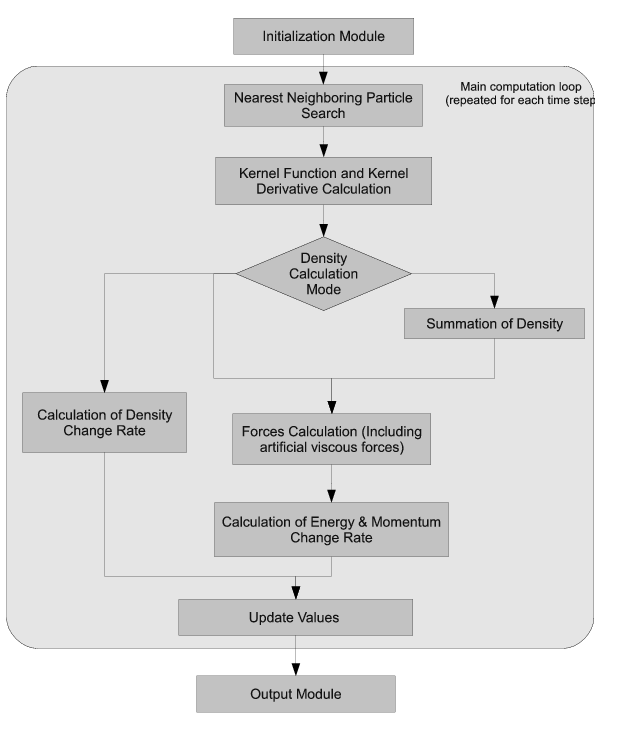
\includegraphics[width=1.0\textwidth]{Graphics/general_structure_SPH}
  \caption{Basic structure of an SPH code (adapted from \cite{Liu2003}) }
  \label{fig:BasicSphCode}
\end{figure}



\section{Presentation of test cases}
\label{sec:testCases}
 
This section introduces the different test cases, which are used to validate the developped code at the different stages. The general problem setup is presented as well as analytical solutions in case they exist. Otherwise a numerical reference solution is provided.

The reason why this section is placed already here is, that the test problems are sometimes referred to from the code section (\ref{sec:1DSPHcode}),(\ref{sec:2DSPHcode}) and it is preferable if they are introduced before.

Details on initializing the flow--field, running the simulations and post--processing are not given in this section but only in section (\ref{sec:simuSetupTestCases}), after having introduced the numerical codes. The present section merely povides the basis by introducing equations and the general ideas necessary to perform the actual simulation and the post-processing.

\subsection{1D shock--tube}
\label{sec:TestCases_1DshockTube}
As an exact solution is known, the 1D shock-tube is a very common test--case for compressible numerical techniques, especially in the form used by Sod \cite{Sod1978}.

%\subsubsection{Presentation and analytical solution}
 The problem consists of two initially separated (e.g. by a diaphragm) gas--filled tube sections, both in general with different properties, at least different pressure. When at the instant $t_0$ (initial situation shown in fihure (\ref{fig:shockTubeT0})) the separation is removed, a shockwave is propagating into the low--pressure area and a rarefaction is traveling into the high pressure area, both adjusting the pressure to the same intermediate value. This means that at a time $t_1>t_0$ the situation can be presented as in figure (\ref{fig:shockTubeT1}) where the nomenclature from Anderson \cite{Anderson2002} is adopted.

\begin{figure}[h]
    \centering
      %\resizebox{!}{4cm}{% Generated with LaTeXDraw 2.0.8
% Tue Aug 31 14:18:55 PDT 2010
% \usepackage[usenames,dvipsnames]{pstricks}
% \usepackage{epsfig}
% \usepackage{pst-grad} % For gradients
% \usepackage{pst-plot} % For axes
\scalebox{1} % Change this value to rescale the drawing.
{
\begin{pspicture}(0,-1.7167188)(12.2,1.7567188)
\psframe[linewidth=0.04,dimen=outer](12.2,0.7032812)(0.0,-1.7167188)
\usefont{T1}{ppl}{m}{n}
\rput(1.775625,-0.51171875){\pscirclebox[linewidth=0.04]{4}}
\usefont{T1}{ppl}{m}{n}
\rput(10.318125,-0.49171874){\pscirclebox[linewidth=0.04]{1}}
\psline[linewidth=0.04cm](6.18,0.68328124)(6.18,-1.6767187)
\psline[linewidth=0.05cm,linestyle=dashed,dash=0.16cm 0.16cm,arrowsize=0.05291667cm 3.0,arrowlength=1.65,arrowinset=0.0]{<-}(6.2,-0.77671874)(7.36,1.0632813)
\usefont{T1}{ppl}{m}{n}
\rput(7.9,1.4082812){\psframebox[linewidth=0.04,framesep=0.1]{diaphragm}}
\usefont{T1}{ppl}{m}{n}
\rput(1.9523437,0.38828126){high pressure section}
\usefont{T1}{ppl}{m}{n}
\rput(10.131719,0.40828124){low pressure section}
\end{pspicture} 
}

}
      % Generated with LaTeXDraw 2.0.8
% Tue Aug 31 14:18:55 PDT 2010
% \usepackage[usenames,dvipsnames]{pstricks}
% \usepackage{epsfig}
% \usepackage{pst-grad} % For gradients
% \usepackage{pst-plot} % For axes
\scalebox{1} % Change this value to rescale the drawing.
{
\begin{pspicture}(0,-1.7167188)(12.2,1.7567188)
\psframe[linewidth=0.04,dimen=outer](12.2,0.7032812)(0.0,-1.7167188)
\usefont{T1}{ppl}{m}{n}
\rput(1.775625,-0.51171875){\pscirclebox[linewidth=0.04]{4}}
\usefont{T1}{ppl}{m}{n}
\rput(10.318125,-0.49171874){\pscirclebox[linewidth=0.04]{1}}
\psline[linewidth=0.04cm](6.18,0.68328124)(6.18,-1.6767187)
\psline[linewidth=0.05cm,linestyle=dashed,dash=0.16cm 0.16cm,arrowsize=0.05291667cm 3.0,arrowlength=1.65,arrowinset=0.0]{<-}(6.2,-0.77671874)(7.36,1.0632813)
\usefont{T1}{ppl}{m}{n}
\rput(7.9,1.4082812){\psframebox[linewidth=0.04,framesep=0.1]{diaphragm}}
\usefont{T1}{ppl}{m}{n}
\rput(1.9523437,0.38828126){high pressure section}
\usefont{T1}{ppl}{m}{n}
\rput(10.131719,0.40828124){low pressure section}
\end{pspicture} 
}

      
      \caption{Shock--tube at initial time $t_0$}
      \label{fig:shockTubeT0}
\vspace*{0.3cm}
      % Generated with LaTeXDraw 2.0.8
% Tue Aug 31 14:32:35 PDT 2010
% \usepackage[usenames,dvipsnames]{pstricks}
% \usepackage{epsfig}
% \usepackage{pst-grad} % For gradients
% \usepackage{pst-plot} % For axes
\scalebox{1} % Change this value to rescale the drawing.
{
\begin{pspicture}(0,-1.21)(12.2,1.21)
\psframe[linewidth=0.04,dimen=outer](12.2,1.21)(0.0,-1.21)
\usefont{T1}{ppl}{m}{n}
\rput(1.775625,-0.005){\pscirclebox[linewidth=0.04]{4}}
\usefont{T1}{ppl}{m}{n}
\rput(10.318125,0.035){\pscirclebox[linewidth=0.04]{1}}
\psline[linewidth=0.04cm,linestyle=dashed,dash=0.16cm 0.16cm](6.48,1.11)(6.48,-1.15)
\psline[linewidth=0.04cm](8.7,1.17)(8.7,-1.19)
\usefont{T1}{ppl}{m}{n}
\rput(5.3664064,0.015){\pscirclebox[linewidth=0.04]{3}}
\usefont{T1}{ppl}{m}{n}
\rput(7.5034375,-0.005){\pscirclebox[linewidth=0.04]{2}}
\psline[linewidth=0.02cm](4.5,1.19)(4.5,-1.17)
\psline[linewidth=0.02cm](4.56,1.17)(4.56,-1.19)
\psline[linewidth=0.02cm](4.62,1.19)(4.62,-1.17)
\psline[linewidth=0.02cm](4.68,1.17)(4.68,-1.19)
\end{pspicture} 
}


      \caption{Shock--tube at time $t_1>t_0$}
      \label{fig:shockTubeT1}
\end{figure}

In figure (\ref{fig:shockTubeT1}), areas 2 and 3 are separated by the so called contact discontinuity, which is the fluid interface generated by the removal of the diaphragm. While in general, the states and properties of the fluids in 2 and 3 are different, pressure $p$ and velocity $u$ at both sides of the discontinuity have to be the same:

\begin{equation}
\begin{split}
\label{eq:condCD}
p_2&=p_3\\
u_3&=u_2
\end{split}
\end{equation}

The analytical solution to the shock--tube problem can be found using the shock relations and the isentropical relations and is taken from Anderson \cite{Anderson2002} as well. 
It will be presented here, as the post processing program, which is described below, is based on this solution.

First the unknown quantities in areas 2 and 3 are calculated (states 1 and 4 are completely known). Then the location of all area boundaries is determined at a certain instant $t_1>t_0$. Finally the properties inside the rarefaction (located between area 3 and 4) can be obtained.

\paragraph{Determination of quantities in areas 2 and 3}

With the relation

\begin{equation}
 \frac{p_4}{p_1} = \frac{p_2}{p_1}  \left(1-\frac{(\gamma_4-1)\frac{c_1}{c_4}\left(\frac{p_2}{p_1}-1\right)}{\sqrt{2\gamma_1\left(2 \gamma_1+(\gamma_1+1)\left(\frac{p_2}{p_1}-1\right)\right)}}\right)^{\left(\frac{-2 \gamma_4}{\gamma_4-1}\right)}
\end{equation}

 the unknown pressure $p_2$ can be determined iteratively, where the sound speed for an ideal gas is calculated according to equation (\ref{eq:soundSpeed}). 

For the further proceeding, the ratio of specific heats $\gamma$ is assumed constant (i.e. same gas in 1 and 4 and besides, no variation of $\gamma$ with temperature)

\begin{equation}
 \gamma_4= \gamma_3= \gamma_2= \gamma_1=const
\end{equation}

The density in area 2 can be determined from state 1 with the shock relations 
\begin{equation}
 \rho_2=\rho_1\frac{1+\frac{\gamma+1}{\gamma-1}\frac{p_2}{p_1}}{\frac{\gamma+1}{\gamma-1}+\frac{p_2}{p_1}}
\end{equation}

Applying the isentropical relations from state 4, one obtains the density in area 3

\begin{equation}
\rho_3=\left(\frac{p_3}{p_4}\right)^{\frac{1}{\gamma}}\rho_4
\end{equation}

The internal energy in areas 2 and 3 is obtained by the ideal gas equation of state (\ref{eq:idealGasEqState}).

The velocity of the shock traveling into area 1 is
\begin{equation}
\label{eq:shockVelocity}
W=c_1\sqrt{\frac{\gamma+1}{2\gamma}\left(\frac{p_2}{p_1}-1\right)+1}
\end{equation}

With the applicaton of the continuity equation, the velocity induced in area 2 $u_2$ by the shock is
\begin{equation}
 u_2=W\left(1-\frac{\rho_1}{\rho_2}\right)
\end{equation}

According to equation \ref{eq:condCD}, the velocity in area 3 $u_3$ is the same.

\paragraph{Determination of the area boundaries at a certain instant}

As geometrical information comes into play, the position of the diaphragm in the space has to be indicated and is assumed to be $x_{dia}=0$ and x is counted positively towards the right, i.e. in direction of the low pressure area (area 1)).
The following positions have to be determined (see also figure \ref{fig:shockTubeT1}:

\begin{enumerate} [(a)]

  \item begin rarefaction (delimits area 4) \\
As the begin of the rarefaction propagates into area 4 with the corresponding (local) soundspeed, its position is 
\begin{equation}
 x_{rar,beg}=-c_4 t
\end{equation}

  \item end rarefaction (delimits area 3) \\
The end of the rarefaction propagates with the corresponding (local) soundspeed relative to the fluid in 3 which itself has a velocity $u_3$. The desired position is therefore
\begin{equation}
 x_{rar,end}=(u_3-c_3) t
\end{equation}

  \item contact discontinuity \\
The contact discontinuity moves with the velocity $u_3$ and therefore
\begin{equation}
 x_{CD}=u_3 t
\end{equation}

  \item shock \\
  The expression for the propagation velocity is given by equation (\ref{eq:shockVelocity}) and therefore
\begin{equation}
 x_{shock}=W t
\end{equation}

\end{enumerate}

\paragraph{Determination of the properties inside the rarefaction}
Inside the rarefaction the flow evolves in an isentropic manner, which means the isentropic relations can be employed. Furthermore, the theory of characteristics gives the velocity at a certain point inside the rarefaction. Again all equations are taken from Anderson \cite{Anderson2002} and the coordinate system remains unchanged: $x=0$ corresponds to diaphragm position and therefore is origin of the rarefaction.

To obtain the velocity inside the rarefactions, the following equation is used
\begin{equation}
 u_{rar}=\frac{2}{\gamma+1}\left(c_4+\frac{x}{t}\right)
\end{equation}

The density at a certain point inside the rarefaction is calculated with
\begin{equation}
\rho=\rho_4 \left(1-\frac{\gamma-1}{2}\frac{u}{a_4}\right)^\frac{2}{\gamma-1}
\end{equation}
and for the pressure, the isentropic relation in the following form is used
\begin{equation}
p=p_4\left(\frac{\rho}{\rho_4}\right)^\gamma
\end{equation}
Finally, the internal energy is computed with the equation of state (\ref{eq:idealGasEqState}).

\subsection{Acoustic wave propagation}
Acoustic phenomena play an important role for the actual problem to be investigated within this project (see chapter (\ref{sec:intro})). It is therefore necessary to get an idea on how the code reproduces these phenomena. A crucial issue in this context is the damping of oscillating or propagating waves due to numerical dissipation: many numerical codes have an intrinsic dissipation, introduced by the numerical scheme, even when the actually implemented equations are inviscid. This numerical dissipation acts like a real viscous dissipation and diminuishes the kinetic energy of the flow. The comparison of the simulation results against the following test cases, whose theoretical solution is always obtained assuming an inviscid flow (i.e. no dissipation), aim at quantifying this damping. A further point to be investigated by means of these test cases is the capability of the code to exactly reproduce the right periodical time $T$ of the propagating/oscillating wave.
%%%%%%%%%%%%%%%%%%%%%%%%%%%%%%%%%%%
%SPH without art. viscosity. does not show any (numerical) damping at all,
% can this be explained somehow by the nature of the method?
%it does not have anything to do with the conservation properties of the method, right???
%momentum conservation: as long as EXTERNAL forces=0 momentum conserved
% and dissipation is internal force...
%energy conservation: dissipation transoforms energy from kinetic to thermal
% so energy is conserved for disssipation processes logically...
 

In order to quantify the effect of viscosity in the simulation results (no matter what nature it is), a damping factor
is introduced as the relative change in amplitude $A$ of two consecutive periods $i$ and $i+1$
\begin{equation}
 f_d=\frac{A_i-A_{i+1}}{A_i}
\end{equation}
where the amplitude $A$ may be measured either in terms of pressure $p$ or velocity $u$.

For the case of a damping force that is proportional to the velocity, the damping factor
is constant. This fact is important with regard to the artificial viscosity that can be included in the code (see section (\ref{sec:ArtVisc})). A closer look at the formulation for the artificial viscosity (equation (\ref{eq:MonArtVis})) yields
\begin{equation}
 \Pi_{ab}\propto v_{ab}
\end{equation}.
This above statement is made assuming $\nu$ from equatio (\ref{eq:MonArtVis}) constant.
%%% WHICH IS actually not at all true, see openoffice-sheet etc...
%%% so, how comes that the damping--factor is constant although the repelling force is not propto the velocity???
%%% am i thinking the wrong way???

%%or perhaps: mue has always about the same value (although globally variable as art. visc. depends on compression/expansion) in the areas where damping occurs (in the compression/expansion zones of the waves) and so, the above statement PI propto velocity is about right



\subsubsection{1D stationnary oscillating wave}
The configuration of an oscillating wave is taken from \cite{Monaghan2005}, where it is used
to study the dispersion relation for an infinite one--dimensional gas. In the present context though, the same configuration is judged suitable for the study of damping and evolution of the periodical time $T$.
Note: in this section, $T$ denotes not the Temperature, but the periodical time! 

The sinusoidal oscillation of wavelength $\lambda$ is initialized by a velocity profile with amplitude of 5\% of sound speed
\begin{equation}
 u(x)=0.05 c\sin\left(\frac{2\pi x}{\lambda}\right)
\end{equation}
in the domain $0\leq x\leq \lambda$ with periodical boundary conditions on both sides.

For a simple harmonic wave, the theoretical periodical time $T$ is given as \cite{Stewart1930}
\begin{equation}
 T=\frac{\lambda}{c}
\end{equation}
and serves as a reference for the comparison with the simulation results.





\subsubsection{1D infinite traveling wave}
This test case is similar to the above one with the difference that now the wave travels in one direction through the space. A theoretical description for this kind of wave can be found using the wave equation for a velocity potential. This is a linearized equation and therefore valid only for small disturbances, which for the present application is justified.
In Stewart \cite{Stewart1930}, the expressions for the fluctuation (denoted by $\delta$) of the desired quantities around their mean values (denoted by the subscript $0$) are directly given and read as follows:
\begin{itemize}
\item velocity evolution 
\begin{equation}
\label{eq:1DWaveDetla_u}
 \delta u(x,t)=k A' \sin(k(ct-x))
\end{equation}
\item density evolution 
\begin{equation}
 \delta \rho(x,t)=\rho_0\frac{k}{c} A'  \sin(k(ct-x))
\end{equation}
\item pressure evolution 
\begin{equation}
 \delta p(x,t)=k c \rho_0 A'  \sin(k(ct-x))
\end{equation}
\item evolution of the displacement $\xi=x-x_0$
\begin{equation}
\label{eq:1DWaveDisplacement}
 \xi(x,t)=-\frac{A' }{c} \cos(k(ct-x))=-\frac{A' }{c} \sin\left(k\left(ct-x+\frac{\pi}{2k}\right)\right)
\end{equation}

\end{itemize}

$A' $ denotes the amplitude of the underlying velocity potential and therefore determines the amplitude of the other quantities as well. It can be any random constant with the restriction that the disturbances in $\rho$ and $p$ remain small compared to their mean value (linear theory). The variable $k$ is the  wavenumber and defined as $k=\frac{2\pi}{\lambda}$.

Furthermore one can note that the displacement is $\pi/2$ or $90^\circ$ in phase ahead of the other quantities. This fact will be important when thinking about the initialization of a finite propagating wave (single wave train). 

For the initialization of the flowfield at the instant $t=0$, the above equations (\ref{eq:1DWaveDetla_u})-(\ref{eq:1DWaveDisplacement}) will be employed (see section (\ref{sec:simuSetupTestCases})).
%%specify exact reference as soon as 1D Wave simu setup is written


\subsubsection{1D wave train with reflection and interference}
For the testing of reflection and interference, the problem as described below is simulated.

But first, some thoughts on the initialization of a single 1D wave train are presented.
Goal is to initialize a 1D wave train in one part of the domain while the rest shall be initialized with unperturbed flow. For this to make any sense, the size of the domain has of course to be superior to the wavelength $\lambda$ of the wave train. 

First attempts to initialize the single wave train using the equations for a continuous (infinite) traveling wave (\ref{eq:1DWaveDetla_u})-(\ref{eq:1DWaveDisplacement}) have turned out to be problematic due to the phase shift between $\rho,p,u$ on the one hand and the displacement $\xi$ on the other hand. As the wave does not continue infinitely but is simply cut off after one wavelength, there will always be a discontinuity in one of the quantities.  

If, for example, the initialization is done with a smooth transition of $\rho,p,u$ from the unperturbed flow, there is a discontinuity in the displacement, and vice versa. This discontunuity (be it in $\rho,p,u$ or in the displacement) constitutes a new disturbance which again is origin of new waves. So, no neat wave train could be created this way. 
Thus, a different way to generate the wave had to be found and it turned out that the periodic movement of a wall boundary was an appropriate mean to do so. 

Now that single wave trains can be produced, the test case is introduced:
A domain with size $l_{\mathit{dom}}$ and limited by two solid walls (at $x=0$ and $x=l_{\mathit{dom}}$) is considered. The left hand wall at $x=0$ has the ability to perform a movement according to a sinusoidal velocity profile, when desired.
The periodical time $T$ of the wave train is chosen in a way that its wavelegth is
$\lambda=l_{\mathit{dom}}/4$. The condition on $T$ is therefore
\begin{equation}
 T=\frac{l_{\mathit{dom}}}{4 c_0}
\end{equation}

The following passage explains the temporal course of the theoretically exact test problem

\begin{itemize} 
\item At $t_0=0$ the left hand side wall begins to move according to 
\begin{equation}
  u_{\mathit{wall}}=u_{\mathit{max}}\sin(\omega t) 
\end{equation}
  where $\omega=\frac{2\Pi}{T}$ and $u_{\mathit{max}}=0.05 c_0$.


\item At $t_1=T$ the wall stops moving, meaning that exactly one wave train has been generated, which now travels through the domain.

\item At $t_2=l_{\mathit{dom}}/c_0$ the first part of the wave train hits the right hand side  wall and starts being reflected. Simultaniously, the LHS wall starts moving again according to same equation as above, generating a new wave.

\item At $t_3=t_2+T$ the LHS wall stops moving and the generation of the second wave is finished. 
The first wave is now completely reflected from the RHS wall.

\item At $t_4=t_3+T$ the two waves begin to interfere. (Both wave trains reach the middle of the domain)

\item At $t_5=t_4+T/2$ the interference of the waves is at maximum, i.e. both waves interfere along their entire wavelength.

\item At $t_6=t_4+T$ the wave interference is over.

\item At $t_7=t_6+T$ both waves hit the respective walls. The test problem ends at this instant.
\end{itemize}


%To get a visual idea of this problem, refer to figure LABEL (show to situations with wave trains...)

\subsection{Taylor--Green flow}

WORK IN PROGRESS 

\subsection{Pure heat--conduction}
 
Solution of two semi infinite solids with same thermal condictivity $k$, same density $\rho$ and same heat capacity $c$ (here: $c=c_v$ as code actually for fluids). Situation where LHS ($x \leq x_m$) of the slab is at $T_l=0$ and RHS ($x > x_m$)at $T_r=const.$ \cite{Carslaw1959}
\begin{equation}
 T(x,t)=\begin{cases}
\frac{1}{2} T_r erfc\left(\frac{|x-x_m|}{2\sqrt{\alpha t}}\right),& \text{for  $x\leq x_m$} \\
\frac{1}{2} T_r\left(1+erf\left(\frac{x-x_m}{2\sqrt{\alpha t}}\right)\right),& \text{for  $x> x_m$}
\end{cases}
\end{equation}
$\alpha=\frac{k}{\rho c}$ is called the thermal difusivity. 

Besides, the energy content of the slab is calculated by summing the internal energy of all the particles and dividing the result by the number of particles
\begin{equation}
 \label{eq:energyContent}
e_{\mathit{domain}}=\frac{1}{N_{\mathit{prtl}}}\sum_i e_i
\end{equation}


WORK IN PROGRESS 

\subsection{compressible Couette--flow}

WORK IN PROGRESS

\section{1D SPH code}
\label{sec:1DSPHcode}

\subsection{Short overview}
%PERHAPS THIS SUBSECTION TITLE IS REMOVED AND THE FOLLOWING TEXT WILL FIGURE JUST BELOW THE SECTION TITLE!?!

This code has a relatively simple structure, yet it features all the components
a more sophisticated SPH computational program would incorporate. Both the summation 
density approach and the continuity density approach are implemented (see section (\ref{sec:DensCalcMode})). By computing a 1D shock--tube problem, the code is used to verify the the basic compressible SPH Euler equations which are then implemented in the more complex 2D program.
 
As the analytical solution for this problem is well known, the shock--tube is a very 
common test case for 1D compressible codes \cite{Sod1978} 
%(PERHAPS ONE MORE REFERENCE WHICH STATES THAT shock-tube IS A COMMONLY USED TEST CASE...). 
The problem setup and the results obtained are discussed in the corresponding section.

\subsection{Components and structure}
\label{sec:CompAndStruc1DCode}
%This section introduces all the...noch ergänzen

\subsubsection{The data structures}

To facilitate the implementation and the handling of the code, two data structures are defined. 

\paragraph{The {\tt parameters} data structure}

This data structure is defined in the header file {\tt parameters.h} and 
contains all parameters needed to set up the problem. Among those parameters are 
geometrical values, the initial conditions, simulation length and time step 
as well as parameters defining the fluid properties.

\paragraph{The {\tt simulation} data structure}

Defined in the file {\tt simulation.h}, this structure is made up of all 
variables that change in the course of the simulation. To begin with, these are the 
values of interest like position, velocity, density, pressure, energy, etc.. 
Furthermore there are variables needed as intermediate results, such as the smoothing 
length and its derivative for example. 
Most of the variables contained in the simulation data structure are needed one per 
particle. Therefore those variables are defined as vectors with a size that corresponds 
to the number of particles in the system. 

\subsubsection{The functions}

As the size of the 1D SPH program is not too big, it admits of the description of every single function used. The textual description is not complete but only comprises particularities and features that are considered worth mentionning. A Nassi-Schneidermann-Diagram (NSD)~\cite{Nassi1973} complements each description and shows the control flow for each function as well as the interdependence of the individual functions. For the sake of a clear illustration, the NSD does not display every loop of the program; frequently, loops over all particles and the interaction list are ommitted (the instruction 'calculate ... for each particle' for example means the implementation of a loop over all particles, i.e., all components of the corresponding variable's vector).  Consulting the comments in the source code is recommended if a more detailed understanding is necessary or desired.

\paragraph{Nassi-Schneidermann-Diagram - a short introduction}
A NSD is employed in this section as it allows for a more compact description of the code structure within limited space than a conventional flow diagram and, in addition, offers a range of further advantages~\cite{Nassi1973}. It is read from top to bottom, with different box symbols representing different kinds of instructions or control elements. The symbols used during the description of the functions below are the following ones:

\subparagraph{The process symbol}

\begin{comment}
there has to be some text, otherwise the parcolumns environment will delete the subparagraph heading!?!
\vspace{5mm}
\begin{parcolumns} [colwidths={1=60mm,2=35mm}] {2}  
 
\colchunk{this symbol represents simple instructions for which during their execution no analysis has to be made. Examples are assignments or inputs/outputs. 
A variation of the conventional process box is the symbol for the call of an external function.} 
\colchunk{

\begin{struktogramm}(40,10)
  \assign[10]{\(Instruction\)}
\end{struktogramm}
\vspace{10mm}
\begin{struktogramm}(30,10)
  \sub[10]{\texttt{function()}}
\end{struktogramm}}

\colplacechunks
\end{parcolumns}
\end{comment}

This symbol represents simple instructions for which during their execution no analysis has to be made. Examples are assignments or inputs/outputs. 
A variation of the conventional process box is the symbol for the call of an external function.
\begin{figure}
\centering
\subfigure[normal Instruction]{
\begin{struktogramm}(50,12)
  \assign[10]{\(Instruction\)}
\end{struktogramm}
}
\subfigure[function call]{
\begin{struktogramm}(50,12)
  \sub[10]{\texttt{function()}}
\end{struktogramm}
}
\caption{The NSD process symbols }
\end{figure}


% \begin{multicols} [colwidths={1=0.6\textwidth,2=0.35\textwidth}] {2}  
%  
% \colchunk{hhhhhhhhhhhhhhhhhhhhhhhhhhhhhhhhhhhhhhhhhhhhhhhhhhhhhhhhhhhhhhhhhhhhhhhhhhhhhhhhhhhhhhhhhhhhhhhhhhhhhhhhhhhhhhhhhhhhhhhhhhhhhhhhhhhhhhhhhhhhhhhhhhhhhhhhhhhhhhhhhhhhh}
% \colchunk{gggggggggggggggggggggggggggggggggggggggggggggggggggggggggggggggggggggggggggggggggg}
% \colplacechunks
% 
% \end{multicols}

\subparagraph{The iteration symbol}
The shown iteration symbol represents loops, where the condition is tested each time before entering the body. This control struct can be implemented by a while loop or a for loop. An example is shown in figure (\ref{NSD_whileLoop}).

\begin{figure}[H]
\centering
\label{NSD_whileLoop}
\begin{struktogramm}(50,22)
\while[10]{\(while \ condition \ true\)}  
\assign[10]{\(body\)}
\whileend
\end{struktogramm}

\caption{The NSD iteration symbol }
\end{figure}

\subparagraph{The decision symbols}
Control structures that depending on a condition enter different branches are represented by the decision symbols. A binary decision symbol corresponding to an if-else statement in programming languages is shown in (FIGURE...). For multi branch control structs, such as if-ifelse-...-else or switch-case, (FIGURE...) provides the corresponding symbol (in the example: 3 branches).
 
\begin{figure}[H]
\centering
\subfigure[binary decision]{	
\begin{struktogramm}(50,22)
\ifthenelse[10]{6}{6}{\(condition \ true?\)}{Y}{N}
\assign[10]{\(subblock\ 1\)}
\change
\assign[10]{\(subblock\ 2\)}
\ifend
\end{struktogramm}
}
\subfigure[multiple decision]{
\begin{struktogramm}(50,22)
  \case[10]{3}{3}{\(test\ X\ \ \)}{cond. 1}
        \assign[10]{\(subblock\ 1\)}
    \switch{2}
        \assign[10]{\(subblock\ 2\)}
    \switch[r]{3~}
      \assign[10]{\(subblock\ 3\)}
   \caseend
\end{struktogramm}
}
\caption{The NSD decision symbols }
\end{figure}
%% allignment of subfigures not exactly at bottomline, could not fix it yet!


%this does work in principle, but the figures are not placed exactly at the right position
% \begin{floatingfigure}[v]{50mm}
% \begin{struktogramm}(20,20)[]
% \assign{\(Instruction\)}
% \end{struktogramm}\caption{test}
% \end{floatingfigure}


Remark: The NSD flowchart language provides the possibility to describe programs at their level of implementation. In the following section however, it is used in a more abstract way and instructions or conditions are verbalized. 
 
\paragraph{The Main function}


As its name suggests, {\tt main.cpp} is the main function of the program. It is entered upon execution of the program, declares and initializes the data structures and calls the functions needed. Its structure is given in figure (\ref{fig:main_structure}).

\begin{figure}[H]
\label{fig:main_structure}
\begin{center}
\begin{struktogramm}(76,27)[MAIN]
  \assign{\(declare \ parameters\ data\ structure\)}
  \assign{\(declare \leq 4 \ simulation\ data\ structure\)}
  %\sub{\begin{verb} setupSim(param, sims) \end{verb}}
  \sub{\texttt{setupSim(param, sims)}}
  %\sub{\begin{verb} \ marchTime(param, sims)\end{verb}}
  \sub{\texttt{marchTime(param, sims)}}
  \assign{\(return\ 0  \ (program\ successfully\ ended)\)}
\end{struktogramm}
\end{center}

\caption{The structure of the main--function}
\end{figure}

\paragraph{The setupSim function}
\label{sec:1DSPHcode_functions_setupSim}

Implemented in the file {\tt setupSim.cpp} with the corresponding header {\tt setupSim.h}, this function represents the 'initialization module' shown in figure (\ref{fig:BasicSphCode}). More precisely, it first sets up the initial particle distribution for the shock--tube problem: depending on the user's selection made by setting the flag 'constspacing', which is a member of the {\tt parameters} data structure, this is done in two different ways:
One possibility is to have an initial particle distribution with the same spacing in the high density area of the shock-tube as in the low density area (flag {\tt constspacing = true}). In this case though, the mass of the particles has then to be adapted to be coherent with the spacing and the initial value of the density.
A second possibility is a particle distribution resulting of a spatially constant particle mass (flag constspacing= false). According to the initial value of the density, the particles will then be further apart in the low density area than in the high density area.
For the further course of the program it is essential that each particle has a unique mean of identification. For more sophisticated 2D or 3D codes, this issue is resolved by explicitely assigning each particle an identification number. For this 1D code however, particle identification is already implicitely given due to the way, the particles and their information are stored: the position, consisting only of an $x$ value, of each particle is stored as one component of a position vector X. Therefore the particles can be clearly identified by the number of the vector component they are stored into.

Once the particles are set up, they are assigned their initial values for the shock-tube problem as choosen in the {\tt parameters.h} file.
\begin{figure}[H]
\label{fig:setupsim_structure}  
\begin{center}
\begin{struktogramm}(115,124)[SETUPSIM]
  \assign{\(Calculate\ LHS \ particle\ spacing\ (dxl)\ based\ on\ constant\ mass\)}
  \assign{\(Calculate\ RHS \ particle\ spacing\ (dxr)\ based\ on\ constant\ mass\)}
  \assign{\(Calculate\ particle\ spacing\ (dx)\ for\ constant\ spacing\)}
  \ifthenelse[10]{6}{6}{\(constspacing\ flag==1?\)}{Y}{N}
    \assign[15]{\(place\ particles\ on\ LHS \ of \)\linebreak \( domain\ starting\ at\ center\ (x=0)\) \linebreak \((with\ distance\ dx)\)}
    \assign[15]{\(place\ particles\ on\ RHS\ of\)\linebreak \( domain\ starting\ at\ x=0\ (with\ distance\ dx)\)}
  \change
    \assign[15]{\(place\ particles\ on\ LHS\ of\ \)\linebreak \( domain\ starting\ at\ x=0\ (with\ dinstance\ dxl)\)}
    \assign[15]{\(place\ particles\ on\ RHS\ of\ \)\linebreak \( domain\ starting\ at\ x=0\ (with\ dinstance\ dxr)\)}
  \ifend
  \assign{\(merge\ particle\ positions\ for\ both\ sides\ into\ one\ vector\ x\)}
  \assign{\(create\ vectors\ with\ initial\ values\ for\ u,\ \rho,\ p,\ e,\ m,\ h\ \)\linebreak \(for\ particles\ on\ LHS \)}
  \assign{\(create\ vectors\ with\ initial\ values\ for\ u,\ \rho,\ p,\ e,\ m,\ h\ \)\linebreak \(for\ particles\ on\ RHS \)}
  \assign{\(merge\ LHS\ and\ RHS\ vectors\ into\ single\ vector\ for\ each\ variable\)}
  \ifthenelse[10]{6}{1}{\(constspacing\ flag\ ==\ 1?\)}{Y}{N}
    \assign{\(calculate\ mass\ for\ particles\ on\ left\ hand\ side\)}
    \assign{\(calculate\ mass\ for\ particles\ on\ right\ hand\ side\)}
    \assign{\(merge\ mass\ values\ into\ one\ single\ vector\ \)\linebreak \((overwrite\ mass\ vector\ from\ above)\)}
  \change
  \ifend
  \assign{\(initialize\ vectors\ for\ derivatives\ \ du,\ de,\ d\rho \)}
\end{struktogramm}
\end{center}

\caption{The structure of the setupSim--function}
\end{figure}


\paragraph{The marchTime function}

The marchTime function conducts the numerical integration using the leapfrog scheme described in section (\ref{sec:numIntegr}). If the program runs in the continuity density mode (flag sumdensity = false), the density is integrated as well, whereas if the program runs in the summation density mode (flag sumdensity = true) the density is smoothed. The latter operation is not performed directly in this function but in one of the (sub)functions that it calls.

\begin{figure}[H]
\label{fig:MarchTime_structure}  

\begin{center}
% \sProofOn
     \begin{struktogramm}(115,134)[MARCHTIME]
  \assign{\(initialize\ vectors\ for\ intermediate\ values\ of\  \rho,\ u,\ e\)}
  \while[10]{\(while\ current\ time\ step\ \leq \ number\ of\ total\ time\ steps\)}
    \ifthenelse[10]{6}{1}{\(current\ time\ step\ \neq1\)}{Y}{~N}
      \assign{\(save\ values\ for\ u,\ e\ in\ their\ intermediate\ variables\)}
      \ifthenelse[10]{6}{1}{\(sumdensity\ flag\ \neq1?\)}{Y}{~N}
        \assign{\(save\ \rho\ value\ in\ its\ intermediate\ vector\)}
        \assign{\(calculate\ new\ \rho\ (+0.5dt)\ by\ integration\)}
      \change
      \ifend
      \assign{\(calculate\ new\ u,\ e\ (+0.5dt) \)\linebreak \(\ by\ integration\)}
    \change
    \ifend
    \sub{\texttt{calcDerivatives()}}
    \ifthenelse[10]{6}{6}{\(current\ time\ step\ ==1?\)}{Y}{N}
      \ifthenelse{6}{1}{\(s.d. \neq1?\)}{Y}{~N}
        \assign[10]{\(calculate\ new\ \rho\ (+0.5dt)\ \)\linebreak \(\ by\ integration\)}
      \change
      \ifend
      \assign[10]{\(calculate\ new\ u,\ e\ (+0.5dt)\)\linebreak\(\ by\ integration\)}
      \assign[10]{\(calculate\ new\ x\ (+1.0dt)\)\linebreak\((advance\ particles\ 1\ timestep)\)}
    \change
      \ifthenelse{6}{1}{\(s.d. \neq1?\)}{Y}{~N}
        \assign[10]{\(calculate\ intermediate\ \rho\ \)\linebreak\((+1.0dt)\ by\ integration\)}
      \change
      \ifend
      \assign[10]{\(calculate\ intermediate\ u,\ e\ \)\linebreak\((+1.0dt) by\ integration\)}
      \assign[10]{\(claculate\ new\ x(+1.0dt)\) \linebreak\((advance\ particles\ 1\ timestep)\)}
    \ifend
    \ifthenelse[10]{6}{6}{\(current\ timestep\ \%\ printstep\ ==0?\)}{Y}{N}
      \sub{\texttt{plotShock()}}
    \change
    \ifend
    \assign[10]{\(check\ stability\ criterion\ (max\ v\ <\ certain\ limit)\ ?\ \) \linebreak\(and\ if\ necessary:\ exit\ program\)}
  \whileend
     \end{struktogramm}
%\sProofOff
\end{center}

\caption{The structure of the marchTime--function, the abbreviation s.d. in the if--statement designates the sumdensity flag}
\end{figure}

\paragraph{The calcDerivatives function}

This function performs the calculation of the derivatives for the velocity $v$ (equation (\ref{eq:VCR_EulerInclArtVis})), the internal energy $e$ (equation (\ref{eq:ECR_EulerInclArtVis})) and, if the continuity density approach is selected, the density $\rho$ (equation (\ref{eq:DCR_Euler})). Included in equations (\ref{eq:ECR_EulerInclArtVis}) and (\ref{eq:VCR_EulerInclArtVis}) is the artificial viscosity term, which is basically calculated according to equation (\ref{eq:MonArtVis}). For the specific case of a shock-tube problem however, it is usual to apply artificial viscosity only in zones where particles are approaching each other and to set it to zero in zones where particles are receding. This ensures that the artificial viscosity is used for shocks and not for rarefactions \cite{Monaghan2005}. As the described 1D SPH code is exclusively applied to a shock-tube problem, this fact has to be taken into account. 
The criterion for not--receding particles being 
%(as there is a $\leq$ in Monaghan05 and not a pure <)
\begin{equation}
 v_{ab}\cdot r_{ab}\leq 0
\end{equation}
the final expression for the artificial viscosity in this 1D shock-tube program is
\begin{equation}
\Pi_{ab}=\begin{cases}
\text{eq. (\ref{eq:MonArtVis})}, &  \text{for~} v_{ab}\cdot r_{ab}\leq 0 \\
0,&  \text{for~} v_{ab}\cdot r_{ab}> 0 
\end{cases}
\end{equation}


\begin{figure}[H]
\label{fig:CalcDerivatives_structure}  


\begin{center}
%\sProofOn
\begin{struktogramm}(115,112)[CALCDERIVATIVES]
  \assign{\(declare\ and\ initialize\ the\ needed\ variables\)}
  \assign{\(reset\ the\ vectors\ d\rho,\ de,\ du\ for\ the\ change\ rates\ to\ zero\)}
  \sub{\texttt{calcBuddies()}}
  \ifthenelse[10]{6}{1}{\(sumdensity==1\ or\ first\ time\ step?\ \)}{Y}{N}
    \assign{\(calculate\ \rho\ by\ smoothing:\) \\ \(-\ calculate\ self\ contribution\ for\ each\ particle\ \) \\ \( -\ calculate\ pair\ contribution\)}
  \change
  \ifend
  \assign{\(calculate\ p\ and\ c\ for\ each\ particle\)}
  \while[10]{\(for\ loop\ to\ iterate\ interaction\ list\ for\ calculation\ of\ change\ rates\)}
    \assign{\(calculate\ values\ needed\ for\ art.\ viscosity\ and\ change\ rates\)}
    \ifthenelse[10]{6}{6}{\(interaction\ pair\ in\ compression?\)}{Y}{N}
      \assign{\(calculate\ art.\ viscosity\ \Pi_{ab}\)}
    \change
      \assign{\(set\ art.\ viscosity\ \Pi_{ab}\ to\ zero\)}
    \ifend
    \assign{\(calculate\ contribution\ of\ current\ interaction\ pair\ to\ \)\linebreak\(change\ rates\ du,\ de\ for\ each\ particle\)}
    \ifthenelse[10]{6}{1}{\(sumdensity\ \neq1?\)}{Y}{N}
      \assign{\(calculate\ contribution\ of\ interaction\ pair\ to\)\linebreak\( change\ rate\ d\rho\ for\ each\ particle\)}
    \change
    \ifend
    \assign{\(add\ contributions\ of\ change\ rates\ to\ the\ change\ rate\ variables\ \) \linebreak\((in\ the\ appropriate\ component\ of\ the\ change\ rate\ vectors)\)}
  \whileend
\end{struktogramm}
%\sProofOff
\end{center}

\caption{The structure of the calcDerivatives--function}
\end{figure}

\paragraph{The calcBuddies function}
This function conducts the nearest neighboring particle search as described in section (\ref{sec:NNPS}) using the pairwise interaction method. If two particles $i$ and $j$ constitute an interaction pair, their unique particle ID (see section (\ref{sec:1DSPHcode_functions_setupSim})) is stored in the same component of the vectors pairi and pairj respectively. pairi and pairj belong to the {\tt simulation} data structure.

\begin{figure}[H]
\label{fig:CalcBuddies_structure}  

\begin{center}
%\sProofOn 
\begin{struktogramm}(115,70)[CALCBUDDIES]
  \assign{\(initialize\ or\ reset\ the\ varibales\ to\ zero\)} %\)\\\((components\ of\ the\ two\ vectors\ pairi,\ pairj\ constituing\ the\ interaction\ list,\)\\ \(\ the\ counter\ for\ the\ total\ number\ if\ interactions,\ \) \\ \(the\ vectors\ containing\ w\ dW\ for\ each\ interaction\ pair,\)\\ \(...)\)}
  \while[10]{\(loop\ from\ first\ to\ penultimate\ particle:\ counter\ i \)}
    \while[10]{\(loop\ from\ second\ to\ last\ particle:\ counter\ j \)}
      \ifthenelse[10]{6}{1}{\(are\ particles\ interacting?\)}{Y}{~N}
        \assign{\(increment\ counter\ of\ total\ interactions\ niac\)}
        \assign{\(save\ the\ particle's\ IDs\ in\ vectors\ pairi\ and\ pairj\)}
        \assign{\(calculate\ kernel\ value\ W_{ab}\ and\ derivative\ dW_{ab}\)\\\( for\ interaction\ pair\)}
        \ifthenelse[10]{6}{1}{\(niac\ \geq max.\ admissible?\)}{Y}{~N}
          \assign{\(output\ message\ on\ screen,\ exit\ program\)}
        \change
        \ifend
      \change
      \ifend
    \whileend
  \whileend
\end{struktogramm}
%\sProofOff
\end{center}

\caption{The structure of the calcBuddies--function}
\end{figure}


\paragraph{The W function}
The W() function implements the smoothing kernel for the SPH method, which in this case is the cubic spline kernel (see section (\ref{sec:KernelFunction})). For implementation purposes the expression of this kernel function (eq. (\ref{eq:cubicSpline})) has been expanded resulting in

\begin{equation}
\label{eq:cubicSplineImplement}
M_{4}(x)=\begin{cases}
\frac{2}{3}-q^{2}+0,5q^{3},& \text{for 0 $\leq$ q $\leq$ 1} \\
\frac{1}{6}(2-q)^{3},&  \text{for 1 $\leq$ q $\leq$ 2} \\
O,& \text{for q $>$ 2}
\end{cases}
\end{equation}


\begin{figure}[H]
\label{fig:W_structure}  

\begin{center}
%\sProofOn
\begin{struktogramm}(100,30)[W]
  \case[15]{3}{3}{\(test\ distance ~ ~~~ ~~ ~ ~ ~ ~ ~ ~ ~ ~ \)}{\(~~is\ distance\ >2?\)}
        \assign[10]{\(W\ according\ to \ \)\\(eq:\ref{eq:cubicSplineImplement})}
    \switch{\(~~<1?\)}
        \assign[10]{\(W\ according\ to \ \)\\(eq:\ref{eq:cubicSplineImplement})}
    \switch[r]{\(else   ~ ~~ ~\)}
      \assign[10]{\(W\ according\ to \ \)\\(eq:\ref{eq:cubicSplineImplement})}
    \caseend
  \assign{\(return\ W\)}
\end{struktogramm}
%\sProofOff
\end{center}

\caption{The structure of the W--function}
\end{figure}

\paragraph{The dW function}
The derivative of the smoothing kernel $\frac{dW}{dx}$ (in 1D) is calculated by this function. Based on the definition of the cubic Spline Kernel(\ref{eq:cubicSpline}), this derivative can be determined easily as

\begin{equation}
\label{eq:cubicSplineDer}
M_{4}(x)=\begin{cases}
\-2q+1,5q^2,& \text{for 0 $\leq$ q $\leq$ 1} \\
-\frac{1}{2}(2-q)^{2},&  \text{for 1 $\leq$ q $\leq$ 2} \\
O,& \text{for q $>$ 2}
\end{cases}
\end{equation}


\begin{figure}[H]
\label{fig:dW_structure}  

\begin{center}
\sProofOn
\begin{struktogramm}(100,29)[dW]
  \case[15]{3}{3}{\(test\ distance ~ ~~~ ~~ ~ ~ ~ ~ ~ ~ ~ ~ \)}{\(~~is\ distance\ >2?\)}
        \assign{\(dW\ according\ to \ \)\\(eq:\ref{eq:cubicSplineImplement})}
    \switch{\(~~<1?\)}
        \assign{\(dW\ according\ to \ \)\\(eq:\ref{eq:cubicSplineImplement})}
    \switch[r]{\(else   ~ ~~ ~\)}
      \assign{\(dW\ according\ to \ \)\\(eq:\ref{eq:cubicSplineImplement})}
    \caseend
  \assign{\(return\ dW\)}

\end{struktogramm}
\sProofOff
\end{center}

\caption{The structure of the dW--function}
\end{figure}


\paragraph{The plotShock function}
This function corresponds to the output module as shown in figure  (\ref{fig:BasicSphCode}) and writes the simulation results at a certain time step in a file named {\tt dataStepxxxxxx.txt}, where xxxxxx indicates the corresponding number of timesteps. The frequency of the output can be choosen by editing the parameter {\tt printstep} of the {\tt parameter} data structure. Each output file has the following format:

$x$ $\rho$ $p$ $u$ $e$
%(one line for each particle)
%(INSERT A TABLE FOR THE FILE STRUCTURE OR DIRECTLY A CAPTION OF THE TXT FILE...)
%\vspace{5mm}

\begin{figure}[H]
\label{fig:plotShock_structure}  

\begin{center}
\sProofOn
\begin{struktogramm}(115,57)[PLOTSHOCK]
  \assign{\(create\ name\ for\ the\ output\ file\ ('dataStepxxxxxx.dat')\)}
  \assign{\(create\ outputfile\ itself\)}
  \while[10]{\(loop\ over\ all\ particles\ (i=0\ until\ i<np)\)}
    \assign{\(output\ component\ i\ of\ the\ position\ vector\ in\ file\)}
    \assign{\(output\ component\ i\ of\ the\ density\ vector\ in\ file\)}
    \assign{\(output\ component\ i\ of\ the\ pressure\ vector\ in\ file\)}
    \assign{\(output\ component\ i\ of\ the\ velocity\ vector\ in\ file\)}
    \assign{\(output\ component\ i\ of\ the\ internal\ energy\ vector\ in\ file\)}
    \assign{\(linebreak\ in\ file\)}
    \assign{\(increment\ i\ (next\ particle\)}
  \whileend
\end{struktogramm}
\sProofOff
\end{center}

\caption{The structure of the plotShock--function}
\end{figure}

\subsection{How to install and run the program}
Installation.
An actual installation is not necessary for the 1D SPH--code, but only the directory {\tt 1DSPH} has to be present on the computer which is supposed to use the code. The directory can either be copied from the attached disc or downloaded from the public git--repository 1DSPH. Git (www.github.com) is a code--hosting and collaboration management tool. The git--repository can be cloned to the local disc by typing the command (provided git is installed on the local computer):
\\
\\
WORK IN PROGRESS

\section{2D SPH code}
\label{sec:2DSPHcode}
\subsection{Short overview}
\label{sec:shortOverview2D}
The 2D SPH code is more sophisticated than the formerly introduced 1D code. Features such as different types of boundary conditions, a more complex and more efficient neighbouring particle search allgorithm, physical viscosity description and heat conduction, as well as an automatic time stepping control are implemented. Thus, this program is more flexible and can be used to treat problems of real scientific and practical importance. 

Just like the 1D SPH code, the 2D code is implemented in C/C++. While the 1D code is still using a functional programming approach, the 2D code follows the object-oriented programming paradigm.

But before starting to describe the structure of the code including all the objects and their interaction (subject of the following paragraphs), a short introduction on the file structure of the whole repository, which containins code, pre-- and post--processing scripts, results etc. is given.

The main folder is called {\tt sph-blitz} and contains a number of sub--folders. Those that are important for the use of the program, are briefly detailed here. The others contain different add--ins and third--party libraries for the program, but their detailed knowledge is not required.
While information on how to install and run the program is given in the corresponding section (\ref{sec:HowToInstAndRun2D}), the present description shall be considered as a first orientation guide. It should help the user to get a rough idea on where to find what.
\begin{itemize}
 \item {\tt src}\\
This folder contains the source code of the C++ program. It has again several subfolders, some of which with further source-files that have been grouped together.
Furthermore it might contain a folder {\tt html}. This folder hosts the code--documentation, which has automatically been created by a corresponding program. If this folder is not existing, one has to run this program to recreate the most up--to--date documentation of the code. Refer to further below in this section for more information.
Finally there is also a folder {\tt outdata}, where the simulation results are written to. This folder might not exist by default. In this case, it is automatically created during simulation. 
\item {\tt scripts}\\
Scripts necessary for pre--processing (generation of initial particle distributions) as well as for post--processing  are arranged in this folder.
\item{\tt gnuplot}\\
Gnuplot being the name of a plotting--software, this folder contains gnuplot--scripts for visualization of the results.
\item{\tt results}\\
The post--processed results for all the simulations performed and presented in the results--section (\ref{sec:2DSPHcodeResults}) can be found in this folder. 
%{\tt README}--files give additional information on post--processing and 


\end{itemize}
Some of the folders and subfolders contain {\tt README}--files, which can be consulted for more precise information and instructions on the corresponding subject. But before having a look at these, it is recommended to read over section (\ref{sec:HowToInstAndRun2D}), as many issues are adressed there.

If one desires to acquire detailed understading of this code without previous knowledge, the following roadmap is suggested.
\paragraph{How to approach the code without previous knowledge}
\begin{enumerate}
 \item go through section (\ref{sec:FeaturesOfSPH}) to get an idea on which parts a code principally contains and how its general structure looks like (in particular, consider figure(\ref{fig:BasicSphCode})).
\item for a first approach to this specific code, consult sections (\ref{sec:Comp2DCode}) and (\ref{sec:Struc2DCode}).
\item to broaden and deepen understanding of implementation--specific details,
an automatic source code documentation system is set up. It provides very extensive documentation (almost to source code level) of all classes, methods and attributes used in the code and even shows dependencies among them by means of call- and caller-graphs for every method (i.e. which methods call the considered method and which methods does the considered method call).
This documentation tool is called doxygen and is used in the following way:
Run doxygen in a shell placed in the {\tt sph-blitz/src}-folder to generate the documentation in form of html-files. The command, provided doxygen is installed on the computer, is:
\begin{verbatim} doxygen
\end{verbatim}
The html-files are written in a newly created folder {\tt sph-blitz/src/html}. Open the main-page of the documentation (index.html) in a browser. The corresponding command supposing one uses for example a firefox browser is:
\begin{verbatim} firefox html/index.html &
\end{verbatim}
% erwähnen dass außerdem die flow--charts im anhang aufschluss drüber geben können, was wie zusammenhängt, denn die loops (und constructors) werden durch doxygen nicht dargestellt
Now, one can navigate through the documentation.
\item the last step might be (provided such detailed knowledge of the code is desired), to directly have a look in the source files. There is additional documentation by comments which are not exported to doxygen.
\end{enumerate}







\subsection{Components}
\label{sec:Comp2DCode}
The different classes and some essential methods are briefly described, to show how the  features generally introduced in section (\ref{sec:FeaturesOfSPH}) are concretely implemented. For a more complete view of the various classes, their methods and all their attributes, it is recommended to use doxygen, the automatic code documentation tool (see section \ref{sec:shortOverview2D}).
\\
\\
WORK IN PROGRESS



\subsection{Structure}
\label{sec:Struc2DCode}

WORK IN PROGRESS

%\lstinputlisting[language=c++,caption=An example of program listing,captionpos=b]{code/hello.cpp}

\subsection{How to install and run the program}
\label{sec:HowToInstAndRun2D}

WORK IN PROGRESS


\section{Simulation Setup and post-processing for different test cases}
\label{sec:simuSetupTestCases}
To provide users with a quick and complete overview of all the settings employed for the different test cases, they are summarized in two tables for each test case -- one with general simulation settings and one with information on the initial particle distribution and particle properties. This is all contained in the respective simulation setup paragraph. 
Furthermore, there is a paragraph entitled validation methods for each test case. It introduces the respective post--processing procedure and the logic of validation. 

\subsection{Employed Norm Definition}
\label{sec:employedNormDefinition}
Where necessary, the simulation results are compared quantitatively to a reference solution. The error for a certain scalar magnitude $B$ ($B$ might for example be the density $\rho$, the internal ernegy $e$, the  etc.) is computed using the $L_1,L_2$ and $L_\infty$ norms as used in \cite{Novak2007}. 
The local error $E_i$ for each particle $i$ is calculated by 
\begin{equation}
 E_i=(B_{\mathit{ref}}-B_{\mathit{simu}})
\end{equation}
where the subscribts $ref$ and $simu$ denote the reference and simulation solutions respectively.
Then the error norms can be calculated as
\begin{equation}
\label{eq:NormDefinition}
\begin{split}
 & L_1=\frac{1}{\norm{B_{\mathit{char}}}}\nnorm{E}_1=\frac{1}{\norm{B_{\mathit{char}}}}\left(\frac{\sum_i \norm{E_i} C_i }{\sum_i C_i}\right)\\[0.3cm]
& L_2=\frac{1}{\norm{B_{\mathit{char}}}}\nnorm{E}_2=\frac{1}{\norm{B_{\mathit{char}}}}\left(\frac{\sum_i E^2_i C_i }{\sum_i C_i}\right)^{\frac{1}{2}}\\[0.3cm]
& L_\infty=\frac{1}{\norm{B_{\mathit{char}}}}\nnorm{E}_\infty=\frac{1}{\norm{B_{\mathit{char}}}}\max \norm{E_i}
\end{split}
\end{equation}

The normalization factor $\norm{B_{\mathit{char}}}$ is  a characteristic value of the quantity $B$. This value is specific to the problem. Furthermore, the above given definition (eq. (\ref{eq:NormDefinition})) is a general formulation allowing for a weighted error norm calculation. The weight factor $C_i$ can be any reasonable variable. For example taking the particle volume ($C_i=V_i$) one obtains a volume weighted norm. Taking $C_i=1$ simply gives the ordinary norm definition.


\subsection{1D SPH code}
\label{sec:simuSetup1DSPHcode}
The simulation setup for the shock--tube test problem is already integrated in the 1D SPH--code, i.e. no pre--processing and the like has to be done before running the code. 
The parameter--setting, which is used for the simulation, from which the sample result presented in section (\ref{sec:1DSPHcodeResults}) is obtained, are the following:
\\
\\
WORK IN PROGRESS

%TABLE PARAMETERS

%TABLE PARTICLES

\subsection{2D SPH code}

\subsubsection{Shocktube Problem}
\label{sec:2Dshock_simuSetup&Co}
Simulation setups and post-processing methods for the sock--tube problem are given both for a 1D and 2D particle distibution. As furthermore, a perturbation study to assess the influence of a initially non uniform particle distribution is conducted, the method to obtain these initial particle placements and particularities for the postprocessing in this case are presented. 

\paragraph{Simulation Setup}

Table (\ref{tab:SimuSettings_Shock}) resumes the settings and parameter values used to obtain the results presented in section (\ref{sec:2DSPHcodeResults_Shock}). 



\begin{table}[h] % in eckigen Klammern steht die Platzierung, h steht f�r genau hier
\label{tab:SimuSettings_Shock}
\centering

\begin{tabular}[c]{|l c|l c|l c|} % die eckige Klammer steht f�r die Ausrichtung der Tabelle im Text: c steht f�r zentriert
\hline
\hline
\multicolumn{2}{|c|}{\textbf{Base Quantity}} & \multicolumn{2}{|c|}{\textbf{Base Unit}} & \multicolumn{2}{|c|}{\textbf{Base Dimension}}\\
\hline
Name & Symbol & Name & Symbol & Name & Symbol\\
\hline
\hline
length & $l$ & meter & $m$ & length & {\bf L}\\

mass & $m$ & kilogram & $kg$ & mass & {\bf M} \\

time & $t$ & second & $s$ & time & {\bf T}\\

electric current & {$I$, $i$} & ampere & $A$ & electric current & {\bf I}\\

thermodynamic temperature & $T$ & kelvin & $K$ & thermodynamic temperature & $a$\\

amount of substance & $n$ & mole & $mol$ & amount of substances & {\bf N}\\

luminous intensity & $I_V$ & candela & $cd$ & luminous intensity & {\bf J}\\
\hline
\hline
\end{tabular}
\caption[]{Shock--tube simulation settings for the 2D--code}

\end{table}
Remark:Exactly as for the 1D code, no boundary conditions in x-direction are used, i.e the edges of the shock--tube are open. In this context, it has to be considered that the 2D SPH code only supports positive particle positions and in order to give the particles enough space at the edge, to move, the shock--tube is treated in a domain going from $x=1$ to $x=3$ instead of $-1\leq x\leq1$. 

As far as the particle distribution is concerned, 4 different cases have to be distinguished for the shock--tube problem. These are either a constant spacing or a constant mass initialization (see also section (\ref{sec:1DSPHcode_functions_setupSim})) combined with either a 1D or 2D particle distribution.
Figure (\ref{fig:schematicOf_CS_CM_distribution}) resumes the two initialization options for teh case of a purely 1D particle distribution.

FIGURE WITH 1D CS CM PARTICLE DISTRIBUTION

Initiation parameters for 1D constant spacing TABLE
(with parameters valid for constant spacing1D/q1D)


TABLE for 1D constant mass


For the constant mass initialization it is not obvious to find a convenient 2D particle distribution (at least not for the density ratio $\rho_l/\rho_r=8$, which is employed in the previous cases). The reason for this is the following:
To respect the initial density ratio with an constant mass approach ($m_l=m_r$) and supposing $dx=dy$ the initial particle spacings for the left and right hand side need to be in 2D:$dx_r=\sqrt{rho_l/rho_r} dx_l$
At the same time, the number of particles in y direction calculated by $N_{l/r}=cell_size/dy_{l/r}$ must 
be an integer for both sides, as particles have to be placed in the cells in a way that allows for a periodical continuation of the domain in y direction.
For a density ratio of 8, an appropriate particle distribution could not be found. One possibility to avoid this problem, or better to diminuish the effects of the conflict at the cell limit, is to increase the domain size in y direction. But increasing the number of cells in $y$ direction would lead to a considerable increase in calculation time, which is not accepted here. So, it was decided to choose a different density ratio for the reference shock tube case; one which is a square number. As 9 is the closest square number to the original density ration of 8, I picked this one.
This way, both sides can be filled with particles in a way that allows for a periodical continuation of the domain in y direction. And the validity of the study is not affected, as the exact solution, of course, is also calculated for this new shock tube configuration with $\rho_l/\rho_r=9$. 

TABLE 2D const mass

With the 2D constant mass particle initialization for a shock-tube though, an additional discontinuous element is added to rthe simulation: 2 of 3 particle lines from the high density section end at the contact discotinuity without being continued in the low density section. This is not expected to be favouralbe for the simulation results, in a sense that the perfect uniformity in the second direction is lost.


(mention somewhere that simulations are not always performed with optimum cell size in order to get reasonably small variation possibilities of support length)
\linebreak                                                                                                                                   
 \linebreak                                                                                                                                   
                                                                                                                                              
 To obtain an initially perturbed particle field for the perturbation--study, essentially two questions have to be addressed: how exactly should the initial particle distribution be perturbed and how should initialization of their properties, especially their densities, work.         
                                                                                                                                              
 Inspiration on this issue is found in literature, where the effect of disordered particles on the SPH method has already been subject of some scientific publications.                                                                                                                      
 First one should keep in mind a finding by Monaghan \cite{Monaghan2005}, who observed that the actual error in an SPH simulation due to disordered particles is generally less than the one that is estimated when conducting theoretical error considerations with the SPH equations. He sees the reason for this in the fact that SPH particles do not produce short wavelength disorders during a simulation, at least if the particle spacing is much smaller than the dominant lenght scale. Therefore, if for the following perturbation study a randomly perturbed particle field is generated, this is supposed to be the worst case for a real SPH simulation.                                                                  
                                                                                                                                              
 Concerning the particle initialization problem, three interesting papers have been found. Rasio and Shapiro \cite{Rassi1991} calculated a 1D shoch--tube problem with a randomly distributed 3D particle distribution, but it is not specified how this distribution is generated. As he further assumes constant mass particles, it must be supposed that he admitts density fluctuations in the initial particle configuration.          
 In a different paper \cite{Graham2007}, the influence of a random particle initialization for viscous flows is investigated. The approach is to perturb particles from their original position on a regular cartesian grid with a uniformly distributed perturbation of a certain width - the width being a measure of randomness.                                                                                                         
 Finally Quinlan and Basa \cite{Quinlan2006} which study the truncation error of SPH, randomize the initial particle position with a normaly distributed perturbation from a cartesion grid position. In their case particles also have equal mass and the density is calculated with the SPH smoothing (IST DAS DER RICHTIGE BEGRIFF?) formula (see equation (\ref{eq:SumDensity})).                                                       
                                                                                                                                              
 The approach adopted in this project is the following. The particle position is randomized from the original regular grid position by a uniformly distributed perturbation in x-direction and for a 2D particle field also independently in y-direction . The advantage of the uniform perturbation is seen in the fact that the maximum vaule of perturbation is clearly determined, whereas for a normal perturbation, very high values might sporadically occurr thus potentially even leading to a coincidence of two particle positions.                                             
 Thus, the uniform perturbation ensures a higher control of particle positions and for a width of the distribution $<0.5dx$ a coincidence or a overlap of two particles can never happen. As far as the mass initialization is concerned, the initial density value for the shock--tube problem should show no perturbations. The perturbations in particle spacing are therefore compensated by a different and individual mass for each particle. While for 1D particle distribution, the calculation of the respective particle mass can be easily performed by $m=\rho*dx$, for the 2D perturbed particle distribution it is not trivial to assign each particle distribution an area $dx dy$. Constructing the area $dx dy$ by employing the mean distance to the neighbours in each direction ($dx=1/2(dx^-+dx^+),dy=1/2(dy^-+dy^+)$ would not (AT LEAST I THINK SO) result in the exact reproduction of the complete domain as $\sum dxdy\neq domain size$. See respective consideration in Appendix!
 Therefore a similar approach of Quinlan \cite{Quinlan2006} is used, onyl the other way round. Based on the initialized density, the mass of each particle is obtained by application of the SPH smoothing formula: First the volume associated to each particle is calculated according to
 \begin{equation}
  V_i=\frac{1}{\sum_j W_{ij}}
 \end{equation}
 and then the particle mass coresponding to the desired volume is calculated with $m_i=\rho_i V_i$. According to \cite{Espanol2003}, in this case the usm of the particle volumes is not exactly the domain volume either, but the error is very small.

 To be consistent this approach of mass initialization is adopted for the perturbation study of both the 1D and 2D particle distributions.

 These perturbed initial conditions are created by programs named according to the underlying unperturbed distribution with the suffix {\tt RAND} to indicate random particle distribution. They are located in the same folder as the initial condition generators for the unperturbed distributions. The perturbance level can be commanded by the perturbation factor {\tt fac} in the programs themselves, where {\tt fac} is the relative width of the uniformly distributed perturbation to the particle spacing: $\mathit{fac}=\mathit{pert_{max}}/dx$.


\paragraph{Validation Method}
To quantify the errors of the shock--tube simulations, the exact results of the problem are calculated according to section (\ref{sec:TestCases_1DshockTube}). Based on this reference, the $L_1, L_2,L_{\infty}$ errors are computed according to equation (\ref{eq:NormDefinition}).
The characteristic values used to normalize the results are for the density an internal enegry their respective initial values on the high pressure side ($\rho_{\mathit{char}}=\rho_4, e_{\mathit{char}}=e_4$) and for the velocity the one induced by the shock ($u_{\mathit{char}}=u_2=u_3$)
These errors are once calculated taking into account the whole domain ($x=-0.5$ to $x=0.5$). 
As the simulation is expected to resolve the discontinuous shock front only within two to three smoothing lengths, this will essentially influence the global error data. Monaghan \cite{Monaghan2005} therefore states that to evaluate the accuracy of an allogrithm for the shock-tube problem one should rather focus on the after--shock values than on the shock resolution. Therefore two further error norm calculations are conducted: one taking into account only the area between shock and contact discontinuity (area 2 in figure (\ref{fig:shockTubeT1}), and another for the area between contact discontinuity and rarefaction (area 3 in figure (\ref{fig:shockTubeT1}). In oder not to capture any inaccuricies due to low resolution of the area edges, a margin of $2h$ is given at each edge.

All this is technicaly realized by programs contained in the folder {\tt sph-blitz/scripts/postProcessingShockTube} with slighty different procedures for simulations with 1D paricle distributions and 2D particle distribution. While for the 1D particle distribution the exact solution can be evaluated directly at each particle's position, the simulation results of the 2D particle distribution cases are first averaged in the second ($y$) dimension. This way a representative 1D particle distribution, where the particles assume the averaged positions and properties of the original 2D distribution, is obtained and the exact solution can be computed. In order to quantify the difference in properties of the particles in y direction which theoretically should be zero and which would be lost by the averaging, also the variance is computed for each couple of particles that is averaged.

The exact post-processing procedure for each case, including which exact programs to run and how to run them, is explained in a very detailed manner in {\tt sph-blitz/scripts/postProcessingShockTube/README}. If a visualization of the post-processed data is finally desired, there are appropriate scripts in the folder {\tt sph-blitz/gnuplot/shockTube\_1D} or {\tt shochTube\_q1D} depending on wheter the particle distribution is 1D or 2D (q1D for quasi-1D, due to 2D particle distribution).
Again the local {\tt README} provides all necessary information on how to run the scripts and what output they produce.

For the perturbation study, the post-processing procedure is exactly the same if the particle distribution is 1D. In the case of a 2D distribution there is a slight technical difference in the program that calculates the averaged values in the second direction. For details refer to the {\tt README} in the corresponding folder, whcih is the same as for the post--processing in the unperturbed case.




\subsubsection{1D wave}
\subsubsection{Taylor--Green}
\subsubsection{Pure Heat Conduction}

\chapter{Results}
This chapter presents the results obtained with the developed codes. The focus clearly lies on the 2D code which is finally used to simulate the porosity configuration. However, as the 1D code has be introduced in the chapter before, an example of its application to the 1D shock-tube--problem is shown in the following section. It serves for a first qualitative discussion of the shock--tube results that can be obtained with SPH.
The 2D code result section mainly features the results of the previously introduced test--cases (\ref{sec:testCases}) and finally a simulation of the flow in a porosity.

As it is not practical to label every result with all the settings used in the simulation to generate it, these settings are summarized for each test--case in the corresponding paragraph of section (\ref{sec:simuSetupTestCases}).

\section{1D SPH code}
\label{sec:1DSPHcodeResults}
As mentionned above, the 1D SPH--code, which only serves demonstration purposes and does not have any practical use, incorporates the simulation setup for the shock-tube--problem. The code is developed to get familiarized with the SPH implementation and to provide a very simple playground to experiment and find the right set of SPH equations for compressible flows. Figure (\ref{fig:1DSPHresults}) shows the results of a simulation with a constant smoothing length of $h=0.0065$ and a constant mass particle distribution, i.e. with different particle spacings on the LHS and RHS of the shock--tube problem (see paragraph (\ref{sec:1DSPHcode_functions_setupSim})) for an introduction of the two shock--tube--specific particle distributions, namely with constant mass or constant spacing. The complete simulation settings for this example can be found in section (\ref{sec:simuSetup1DSPHcode}). 

\begin{figure}[!htbp]

\centering
\label{fig:1DSPHresults}
\subfigure[]{
\label{fig:1DSPHreultsVelocity}
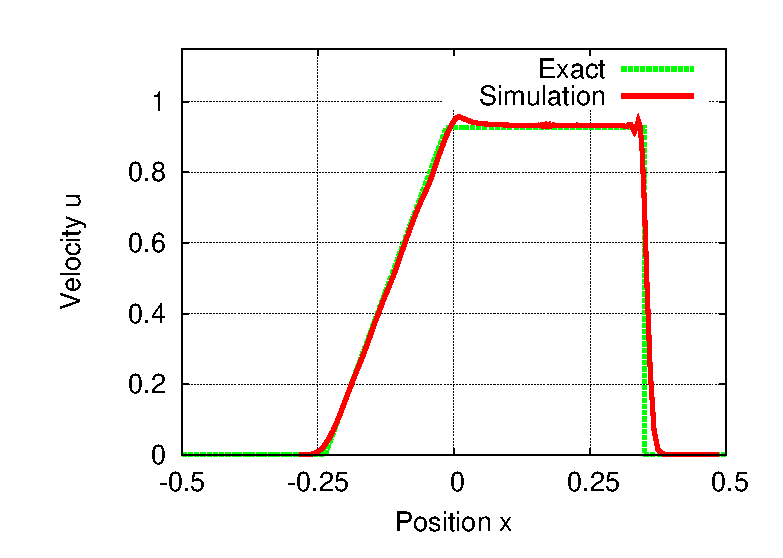
\includegraphics[width=7cm]{Graphics/results/1DCode/velocity}}
\subfigure[]{
\label{fig:1DSPHreultsDensity}
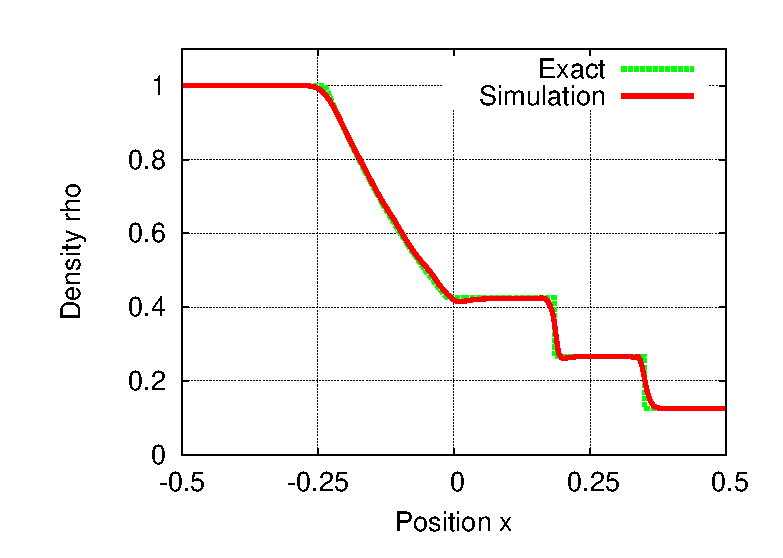
\includegraphics[width=7cm]{Graphics/results/1DCode/density}}
\subfigure[]{
\label{fig:1DSPHreultsPressure}
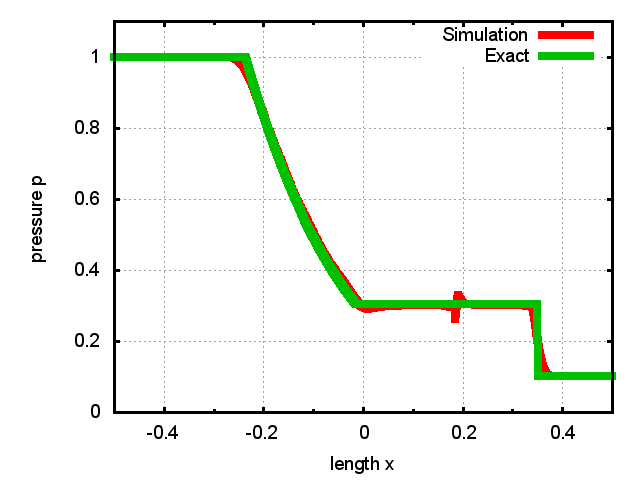
\includegraphics[width=7cm]{Graphics/results/1DCode/pressure}}
\subfigure[]{
\label{fig:1DSPHreultsEnergy}
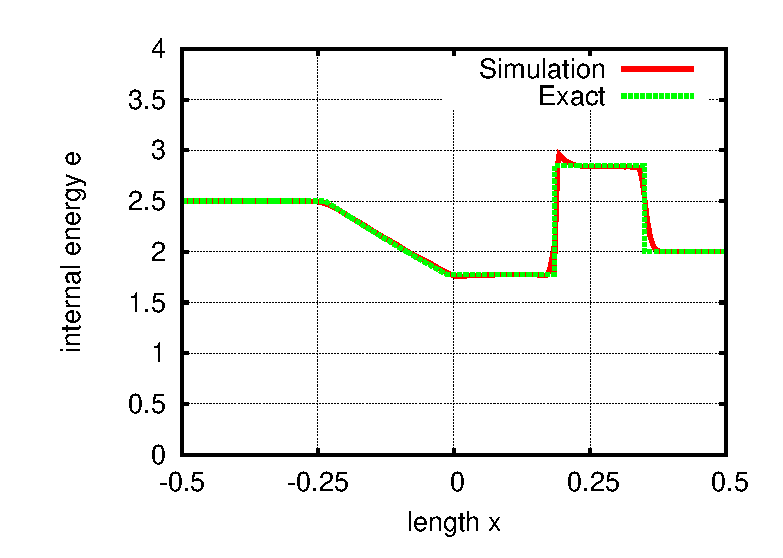
\includegraphics[width=7cm]{Graphics/results/1DCode/energy}}

\caption[Example of a shock-tube result obtained with the 1D SPH--code]{Example of a shock-tube result obtained with the 1D SPH--code for a simulation time of $t=0.2$ contrasted with the exact analytical solution (see section (\ref{sec:TestCases_1DshockTube})): (\subref{fig:1DSPHreultsVelocity}) velocity profile; (\subref{fig:1DSPHreultsDensity}) density profile; (\subref{fig:1DSPHreultsPressure}) pressure profile;(\subref{fig:1DSPHreultsEnergy}) profile of the internal energy.}

\end{figure}

While quantitative evaluation of the shock--tube results will only be done with the 2D code, some qualitative statements can already be made at this place.
Comparison with SPH--solutions from literature shows that the profiles presented in figure (\ref{fig:1DSPHresults}) are typical. Taking for example the results of \cite{Liu2003} or \cite{Monaghan1985} one can observe the same tendencies: the shock front is resolved within several (2-3) smoothing lengths. The same applies for the contact discontinuity in the variables where there are discontinuities ($\rho, e$). Furthermore the fact that the internal energy is overestimated at the high energy side of the contact discontinuity seems to be typical as well and a remedy is found by smoothing the initial energy profile before starting the actual calculation \cite{Monaghan2005,Price2004}. On the other hand by smoothing initial conditions, one looses accuracy in the resolution of the rarefaction \cite{Price2004}.  The oscillations after the shock front (notably in the velocity profile) are normal as well and by the way are one of the reasons why an artificial viscosity has to be used for shock simulations: besides preventing particles from interpenetrating at the shock front, another main function of the arificial viscosity is to dissipate these velocity oscillations \cite{Monaghan2005,Sigalotti2006}.
Finally, the little blib in the pressure profile at the contact discontinuity is known in literature as well. It can be removed by introducing a small amount of heat diffusion into the energy equation \cite{Monaghan1992}. The logic behind the use/effect of this artificial heat diffusion term is the following: the artificial viscosity, which is also taken into account in the energy equation (see section (\ref{sec:ArtVisc})), may produce excessive heating \cite{Sigalotti2006}. This phenomenon is commonly refered to as wall--heating errors (originally discovered by \cite{Noh1978}), and it can be significantly reduced by introducing an atrificial heat diffusion term to the internal energy equation. The exact form of this term however, differs from author to author. Monaghan \cite{Monaghan1992} for example only suggests a constant value of heat diffusion to be added for the shock--tube case. More sophisticated, variable heat diffusion terms are proposed by Price \cite{Price2004} and Sigalotti \cite{Sigalotti2006}.
However, as the wall--heating error only occurrs for strong shocks and as there are no shocks at all expected in the application of this code, which is a high enthalphy flow through porous meida, this ``trick'' is not implemented. 

The first qualitative evaluation of the simulation results implies that the equations used for the compressible 1D SPH code are the good ones and encourages the integration of these equations in the more complex 2D SPH code, where extensive quantitative evaluation is performed.  

%see danial Price2004 Thesis for effect of smoothing: He smoothes rho,p and does not get the energy peak at the discontinuity for the smoothed initial conditions. (I smooth density as well, (and I think pressure is therefore smoothed as well (as recalculated from smoothed density before used anywhere in the program (BUT I HAVE TO CHECK THAT IN THE PROGRAM BEFOR WRITING THE FINAL VERSION))
%I also have to check HOW the variables are smoothed (I smooth rho just by applying the summation formula but Sigalotti2006 uses a different smoothing formula...)
 
%More exact results (falsch, peaks gehn zwar weg, aber dafür rarefaction nur verschmiert aufgelöst!!!) for the shock-tube problem can be obtained by smoothing all initially discontinuous quantities ($\rho, u, e$) at the beginnig of the calculation. This was originally proposed by \cite{Monaghan1997}. Applying a variable smoothing length also improves the results\cite{Monaghan2005}. 







%...Monaghan05 p.1739... not shock width important but pre and after shock values...

\section{2D SPH code}
\label{sec:2DSPHcodeResults}

The 2D SPH code underwent extensive testing at the various stages of development. After modification towards compressible fow capabilities, the shock--tube test case was investigated and propagation of acoustic waves was analyzed. In a subsequent step viscosity implementation has been tested by the taylor-green flow and independently of any flow problem the implemented heat conduction model was verified by a pure conduction test--problem. The compressible couette flow in which different phenomena are combined concludes the testing.

\subsection{shock--tube test case}
\label{sec:2DSPHcodeResults_Shock}
The shock--tube case is used to conduct several series of simulations aimed at the verification of the modified code and at assessing its convergence behaviour (IST DAS NICHT ABHÄNGIG VOM TESTFALL??) as well as the robustness versus perturbabtions in particle positions. 
First, the automatic time step control is exemplarily tested. Then the influence of the two approximation parameters $h$ and $dx$ on the simulation results is shown by means of a resolution study, which consists of two parts. One part where the smoothing length $h$ is varied at constant $dx$ and another part, where the resolution is increased at a constant ratio of $h/dx$. Ultimately, the perturbation study consists of a set of simulations with increasingly perturbed initial particle positions.

All the above tests are conducted for the four cases:
\begin{itemize}
 \item 1D particle distribution with constant spacing
  \item 2D particle distribution with constant spacing
 \item 1D particle distribution with constant mass
  \item 2D particle distribution with constant mass
\end{itemize}

Unless otherwise stated the simulation time for each shock--tube simulation is $t=0.2$. Other simulation settings as well as the entire set of initial conditions can be found in section (\ref{sec:2Dshock_simuSetup&Co}).

The nature of an exemplary shock--tube simulation result including explanations is already given in section (\ref{sec:1DSPHcodeResults}). It is still the same for the 2D code and therefore is not repeated at this place. Instead focus lies clearly on the evaluation of the error norms and profiles are shown only where they exhibit a particularity. However, the complete set of figures for each simulation run constituting the following analyzes can be found in the corresponding {\tt results} folder of {\tt sph-blitz}. The path to the respective folder is given for each of the following sets of simulation.



\subsubsection{Verification of timestep criteria}

In section (\ref{sec:TmeStepChoice}) the criteria for a stable time step choice have been presented. In order to be sure that for the further studies of results, all errors are due to spatial discretization, the applied time stepping criteria are tested for correctness. As the shock--simulation includes artificial, but no real viscosity and no thermal conduction, the criteria in question are equations (\ref{eq:dtForce}) and (\ref{eq:dtCourantVisc}). Figure (\ref{fig:2DSPHresults_1D_CStimeVerif}) shows the evolution of the L-errors (see section (\ref{sec:employedNormDefinition})) for $\rho, u, e$ with varying time step evaluated in the whole domain and in areas 2 and 3 only (see section (\ref{sec:2Dshock_simuSetup&Co}). 
The errors taking into account the whole domain are generally higher than the ones that only focus on the after-rarefaction (area 3) and after-shock (area 2) values. The $L_{\infty}$ error which is not an integral error measure but the maximum value of each particle-wise error is naturally the biggest one, followed by the $L_2$ and then the $L_1$ errors. For the shock--tube case the global $L_{\infty}$ error is entirely determined by the shock--front, where the errors are locally biggest due to the finite shock resolution. Evaluated only for areas 2 or 3 the $L_{\infty}$ error captures often either oscillation maxima or the hangover of the non-exact shock or rarefaction resolution (rarefaction resolution non exact due to initial smoothing of density field) which reaches into the corresponding area.

The considerable increase of the error-values in area 2, particularly in the velocity field, starting at a timestep size of around $dt\geq0.0025$ show that temporal instability is indicated first in the after-shock area. A look at the plotted velocity-profile in figure (\ref{fig:2DSPHresults_dt_variat_oscillationU}) of one of these simulations confirms this, by showing severe oscillations directly after the shock area. It will turn out that the inaccuracy observed in the rarefaction in the same figure is particular to the constant spacing particle initiation, at least in 1D, and has nothing to do with temporal resolution.

\begin{figure}[!htbp]

\centering
\label{fig:2DSPHresults_dt_variat_oscillationU}
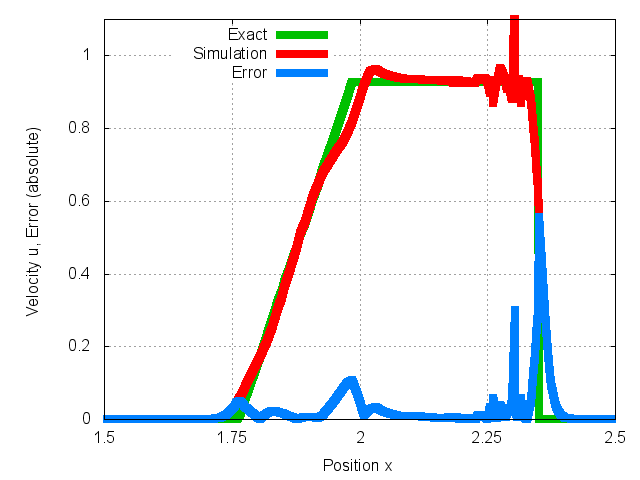
\includegraphics[width=7cm]{Graphics/results/ShockTube/1D_CS_LF_SD/dtVariat_dx005_SupLen03_dt03_Oscillations/Err_u00200000}
\caption[Velocity oscillations due to temporal instability]{Velocity profile after $t=0.2$ for a timestep of $dt=0.002985$, which shows severe oscillations in the after--shock area due to a too big timestep $dt$. The support length of the simulation is $0.03$ with an 1D particle distibution of constant spacing of $dx=0.005$ }

\end{figure}

Concerning the temporal resolution test again, values of $dt<0.0025$ can be considered as stable for this configuration and a look at the automatically determined timestep ($dt=0.00198083$) shows it is just below this critical value, including a decend safety margin.

The residual errors in figure (\ref{fig:2DSPHresults_1D_CStimeVerif}) for $dt<0.0025$ can therefore be attributed to the spatial discretization error due to $dx$ (or better $h/dx$) and integral approximation error due to $h$. All results leading to figure (\ref{fig:2DSPHresults_1D_CStimeVerif}) can be found in {\tt sph-blitz/results/ShockTubeTestCase/1DpartDist\_constSpace\_LeapFrog/dtVariat\_dx005\_SupLen03}.

Another verification has also been conducted for a 2D constant spacing particle resolution. The time stepping criteria worked fine for this case as well. 




\begin{figure}[H]
\centering
\label{fig:2DSPHresults_1D_CStimeVerif}

\subfigure[tight][whole domain]{
\label{fig:2DSPHresults_1D_CStimeVerif_wholeRho}
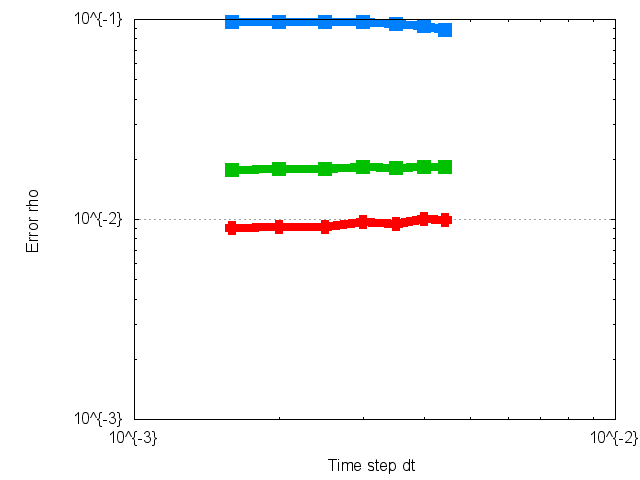
\includegraphics[width=5cm]{Graphics/results/ShockTube/1D_CS_LF_SD/dtVariat_dx005_SupLen03/WholeDomainRho}}
\subfigure[tight][area 3]{
\label{fig:2DSPHresults_1D_CStimeVerif_3Rho}
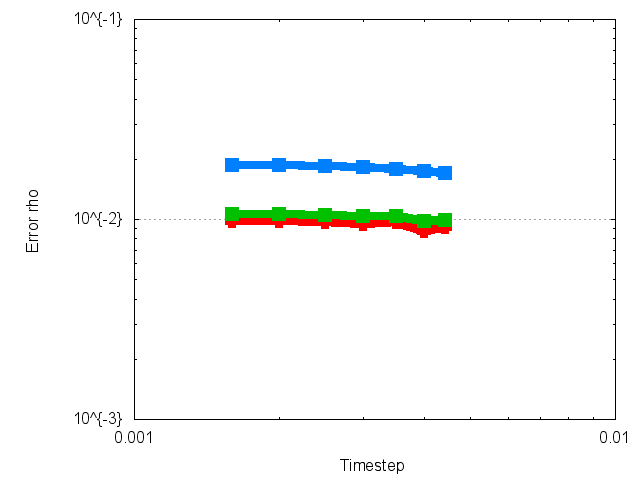
\includegraphics[width=5cm]{Graphics/results/ShockTube/1D_CS_LF_SD/dtVariat_dx005_SupLen03/Area3Rho}}
\subfigure[tight][area 2]{
\label{fig:2DSPHresults_1D_CStimeVerif_2Rho}
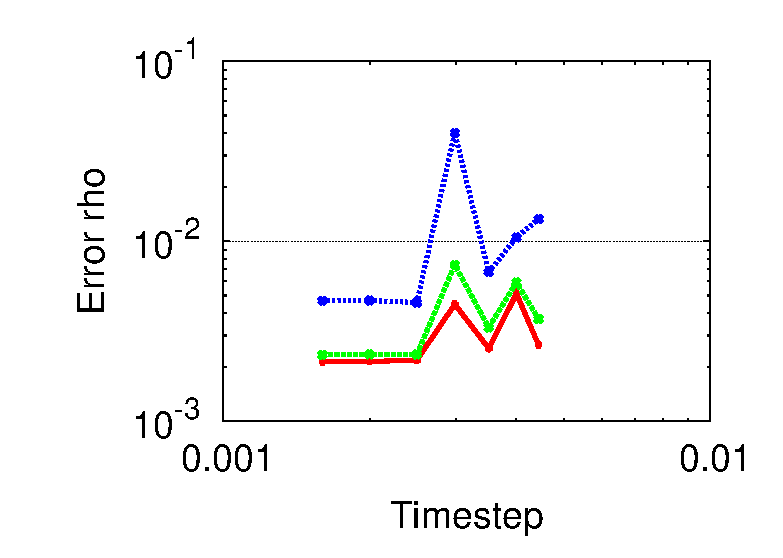
\includegraphics[width=5cm]{Graphics/results/ShockTube/1D_CS_LF_SD/dtVariat_dx005_SupLen03/Area2Rho}}
\subfigure[tight][whole domain]{
\label{fig:2DSPHresults_1D_CStimeVerif_wholeU}
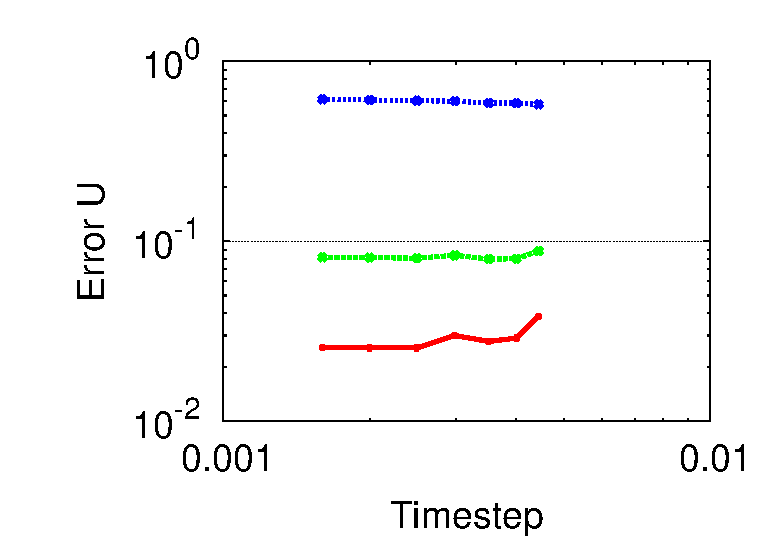
\includegraphics[width=5cm]{Graphics/results/ShockTube/1D_CS_LF_SD/dtVariat_dx005_SupLen03/WholeDomainU}}
\subfigure[tight][area 3]{
\label{fig:2DSPHresults_1D_CStimeVerif_3U}
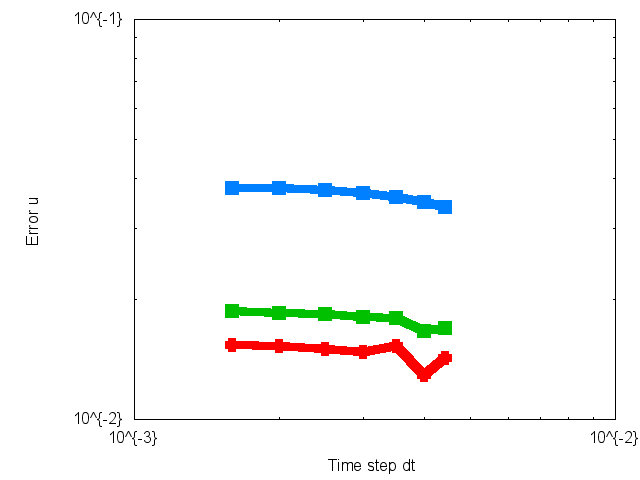
\includegraphics[width=5cm]{Graphics/results/ShockTube/1D_CS_LF_SD/dtVariat_dx005_SupLen03/Area3U}}
\subfigure[tight][area 2]{
\label{fig:2DSPHresults_1D_CStimeVerif_2U}
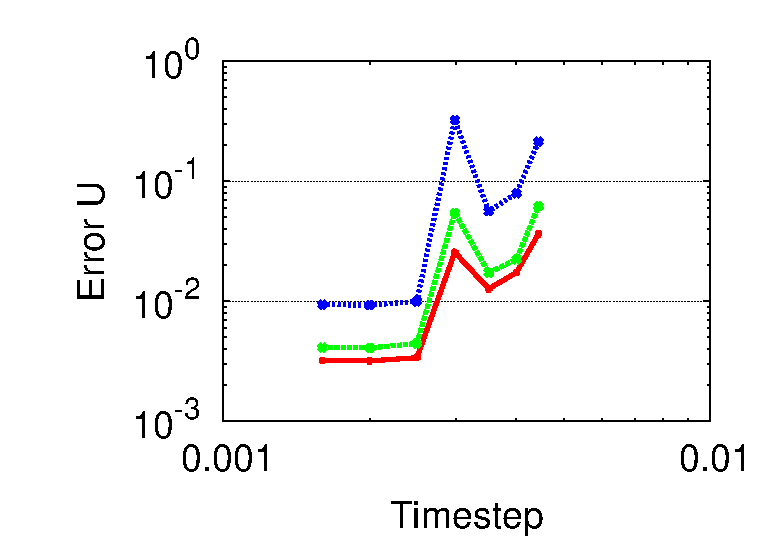
\includegraphics[width=5cm]{Graphics/results/ShockTube/1D_CS_LF_SD/dtVariat_dx005_SupLen03/Area2U}}
\subfigure[tight][whole domain]{
\label{fig:2DSPHresults_1D_CStimeVerif_wholeE}
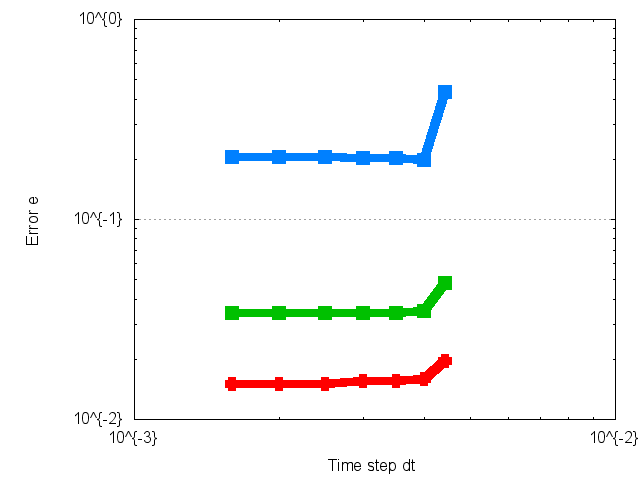
\includegraphics[width=5cm]{Graphics/results/ShockTube/1D_CS_LF_SD/dtVariat_dx005_SupLen03/WholeDomainE}}
\subfigure[tight][area 3]{
\label{fig:2DSPHresults_1D_CStimeVerif_3E}
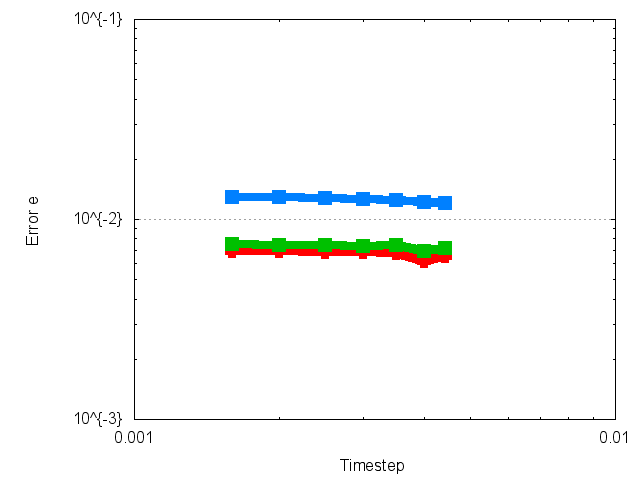
\includegraphics[width=5cm]{Graphics/results/ShockTube/1D_CS_LF_SD/dtVariat_dx005_SupLen03/Area3E}}
\subfigure[tight][area 2]{
\label{fig:2DSPHresults_1D_CStimeVerif_2E}
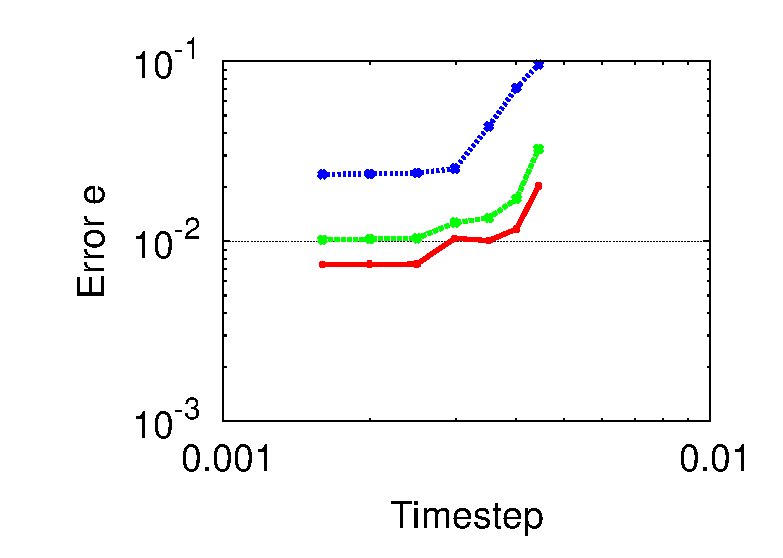
\includegraphics[width=5cm]{Graphics/results/ShockTube/1D_CS_LF_SD/dtVariat_dx005_SupLen03/Area2E}}

\caption[Convergence Shock-tube 1D constant spacing particle distribution]{L--norm errors of $\rho, u, e$ for a series of simulation with a varying time step $dt$. The support length is $0.03$ with an 1D particle distibution of constant spacing of $dx=0.005$}

\end{figure}

\begin{figure}[H]
\centering
\label{fig:2DSPHresults_tempRes_vProfile}

\subfigure[tight][whole domain]{
\label{fig:2DSPHresults_1D_CS_dx_const_wholeRho}
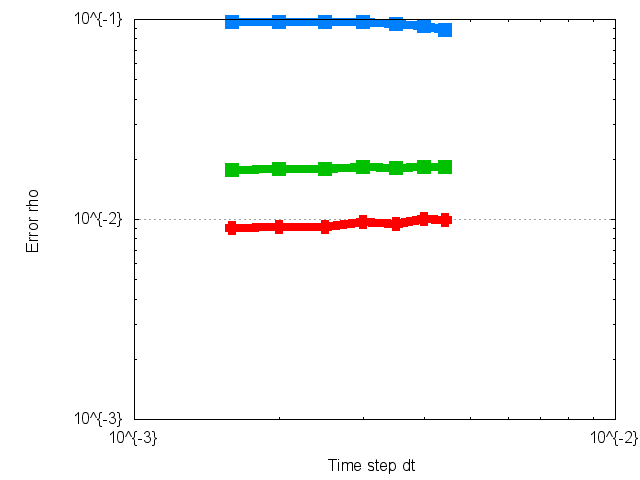
\includegraphics[width=5cm]{Graphics/results/ShockTube/1D_CS_LF_SD/dtVariat_dx005_SupLen03/WholeDomainRho}}
\end{figure}



\subsubsection{Resolution Study - spacing held constant}
\label{sec:2DSPH_results_shock_resSTudy_dx=const}
The purpose of this set of simulations is to evaluate the influence of a smoothinglength variation with a constant particle distance. There is expected to be an optimum value for $h$ in this case: For small $h$, the ratio $h/dx$ and therefore the number of neighbouring particles in the supoprt domain of a certain particle will be to small to ensure a correct discrete representation of the integral interpolant. On the other hand, greater smoothinglengths mean a worse resolution of local phenomena and here especially shocks, which will increase the error considerably. 


\paragraph{1D constant spacing particle distribution}

Having a look at figure (\ref{fig:2DSPHresults_1D_CS_dx_const}), one sees the above anticipated tendency. Especially the integral errors ($L_1,L_2$) calculated for the whole domain show a clear minimum at a supportlength of around 0.025, which means that the number of neighnouring particles is 8. 
The increase of the errors for medium support lengths in area 3 is due to a drift of the inaccuracy in the rarefaction wave into area 3. Otherwise this inaccuracy, which is always present for this set of simulations, is not taken into account for area 3 but only in the global error calculation. 
If the supportlength becomes too big, not only the shock resolution gets poorer, but also the after--shock velocity profile becomes bumpy.

\begin{figure}[H]
\centering
\label{fig:2DSPHresults_1D_CS_dx_const}

\subfigure[tight][whole domain]{
\label{fig:2DSPHresults_1D_CS_dx_const_wholeRho}
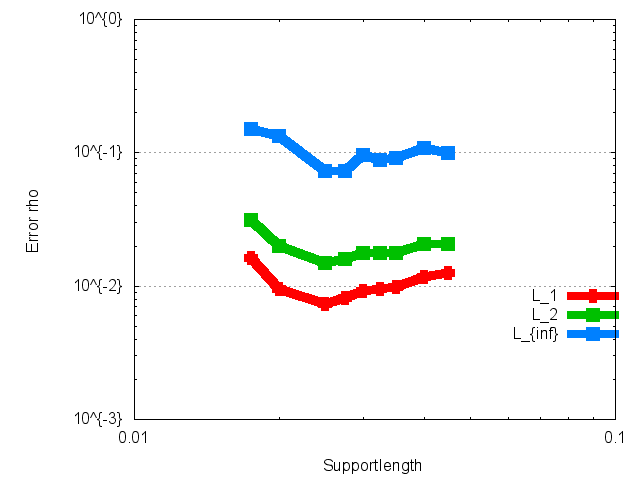
\includegraphics[width=5cm]{Graphics/results/ShockTube/1D_CS_LF_SD/SuppLenVariat_dx005_dt0025/WholeDomainRho}}
\subfigure[tight][whole domain]{
\label{fig:2DSPHresults_1D_CS_dx_const_3Rho}
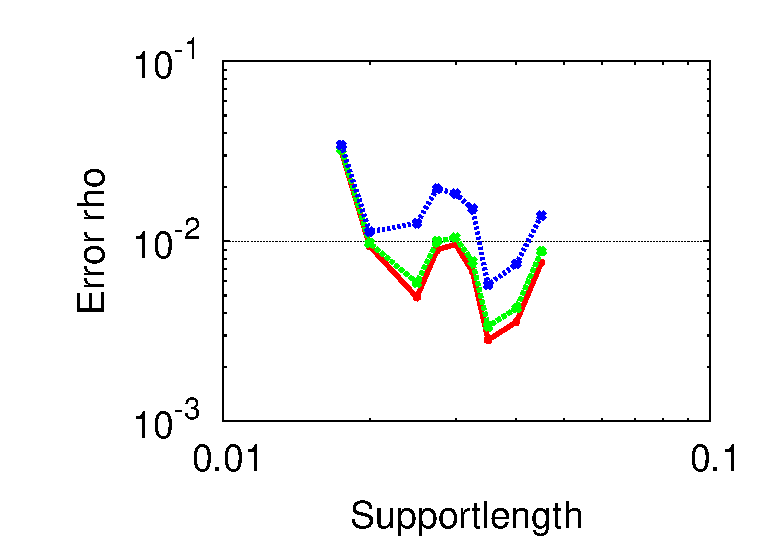
\includegraphics[width=5cm]{Graphics/results/ShockTube/1D_CS_LF_SD/SuppLenVariat_dx005_dt0025/Area3Rho}}
\subfigure[tight][whole domain]{
\label{fig:2DSPHresults_1D_CS_dx_const_2Rho}
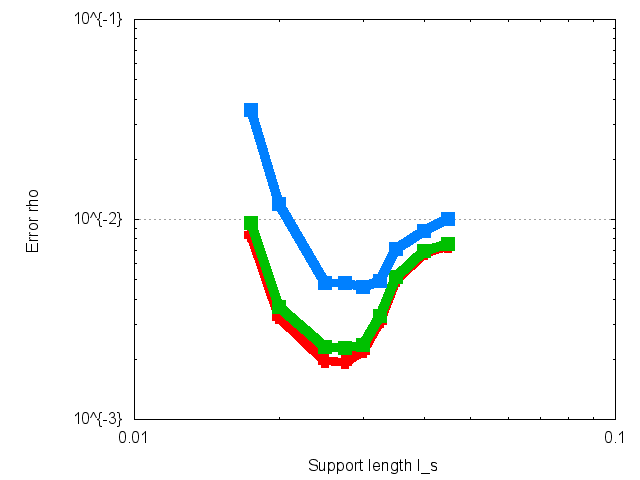
\includegraphics[width=5cm]{Graphics/results/ShockTube/1D_CS_LF_SD/SuppLenVariat_dx005_dt0025/Area2Rho}}
\subfigure[tight][area 3]{
\label{fig:2DSPHresults_1D_CS_dx_const_wholeU}
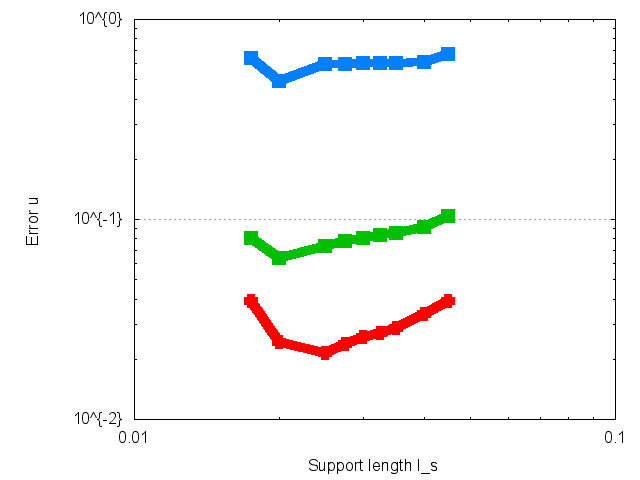
\includegraphics[width=5cm]{Graphics/results/ShockTube/1D_CS_LF_SD/SuppLenVariat_dx005_dt0025/WholeDomainU}}
\subfigure[tight][area 3]{
\label{fig:2DSPHresults_1D_CS_dx_const_3U}
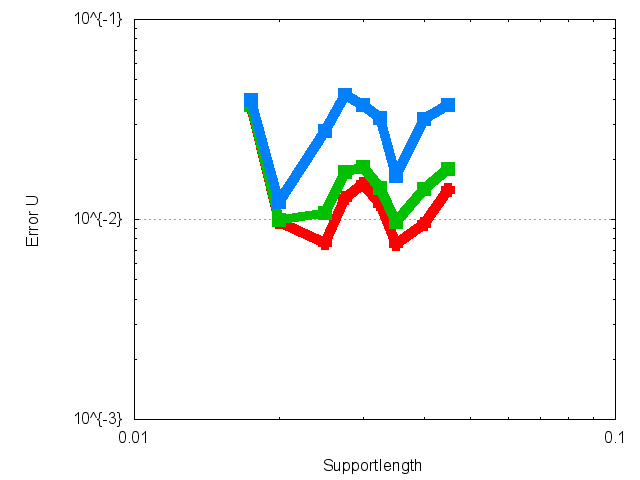
\includegraphics[width=5cm]{Graphics/results/ShockTube/1D_CS_LF_SD/SuppLenVariat_dx005_dt0025/Area3U}}
\subfigure[tight][area 3]{
\label{fig:2DSPHresults_1D_CS_dx_const_2U}
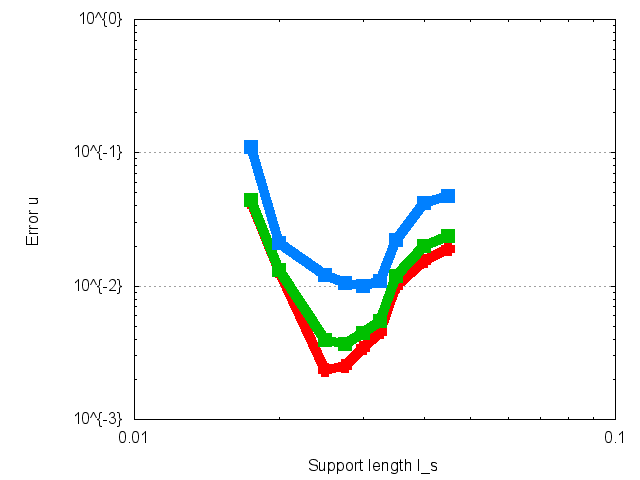
\includegraphics[width=5cm]{Graphics/results/ShockTube/1D_CS_LF_SD/SuppLenVariat_dx005_dt0025/Area2U}}
\subfigure[tight][area 2]{
\label{fig:2DSPHresults_1D_CS_dx_const_wholeE}
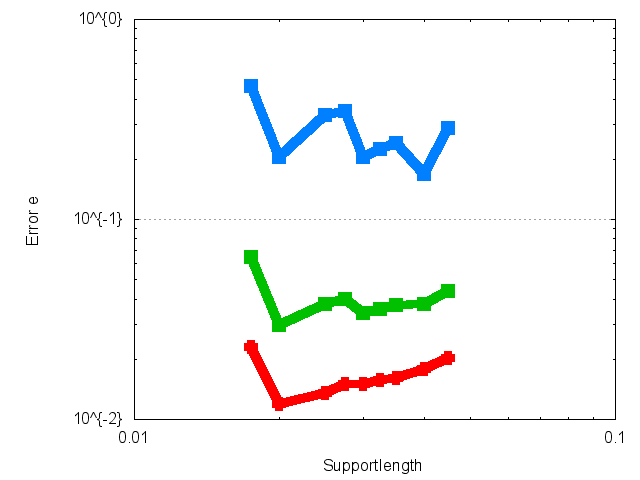
\includegraphics[width=5cm]{Graphics/results/ShockTube/1D_CS_LF_SD/SuppLenVariat_dx005_dt0025/WholeDomainE}}
\subfigure[tight][area 2]{
\label{fig:2DSPHresults_1D_CS_dx_const_3E}
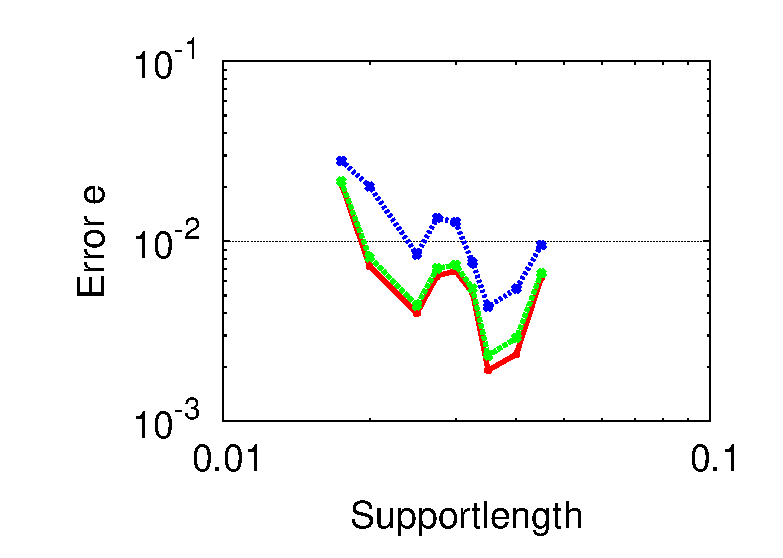
\includegraphics[width=5cm]{Graphics/results/ShockTube/1D_CS_LF_SD/SuppLenVariat_dx005_dt0025/Area3E}}
\subfigure[tight][area 2]{
\label{fig:2DSPHresults_1D_CS_dx_const_2E}
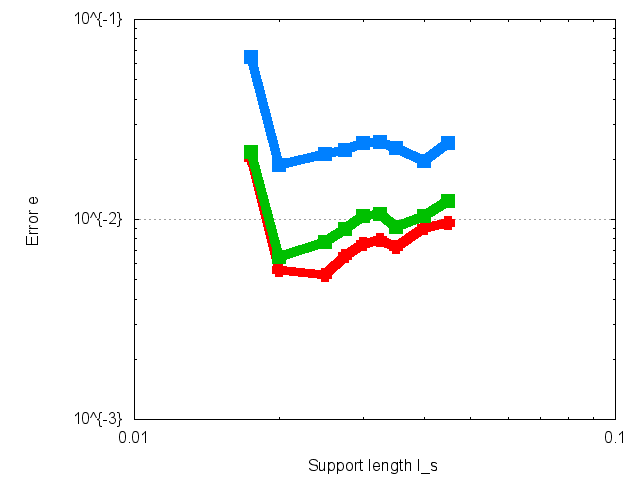
\includegraphics[width=5cm]{Graphics/results/ShockTube/1D_CS_LF_SD/SuppLenVariat_dx005_dt0025/Area2E}}

\caption[Convergence Shock-tube 1D constant spacing particle distribution]{L--norm errors of $\rho, u, e$ for a series of simulation with a varying supoprt length and a constant particle spacing of $dx=0.0025$}

\end{figure}



\paragraph{2D constant spacing particle distribution}

The same procedure as in the paragraph just above is now conducted with a 2D particle distributio of a spacing of $dx=dy=0.005$ and again it is found out that the optimum support length ist around 0.025, like for the corresponding 1D particle distribution. Otherwise the results look the same as in figure (\ref{fig:2DSPHresults_1D_CS_dx_const}) and are therefore only presented in the Appendix.

When having a look at the evolution of the particle positions during a simulation, which is displayed in figure (\ref{fig:2DSPHresults_CS_drifting}) it is remarkable that the particles at the contact discontinuity drift away from their originally perfectly lined up position. However this behaviour seems stable for support lengths $\geq0.02$ (at least within the simulation time of 0.2)(figure (\ref{fig:2DSPHresults_CS_drifting_suplen02}) and is visually not detectable anymore for a support length 0f $\geq0.35$. In the simulation with a supportlength of 0.015 particles around the contact discontinuity are comletely drifting  away from their original position, forming a bizzare structure - it seems as if they were attracted by the symetrically drifting particles of the next row (figure (\ref{fig:2DSPHresults_CS_drifting_suplen015}). 
The drifting is probably an expression of what Monaghan \cite{Monaghan2005} (shocks in 2D/3D can be noise - at least with current allgorithms) and Rasio \& Shapiro \cite{Rasio1991} (in >1D there is a much bigger effect of numerical noise for shock tube simulation) state in their papers.

\begin{figure}[!htbp]
\centering
\label{fig:2DSPHresults_CS_drifting}
\subfigure[supportlength 015]{
\label{fig:2DSPHresults_CS_drifting_suplen015}
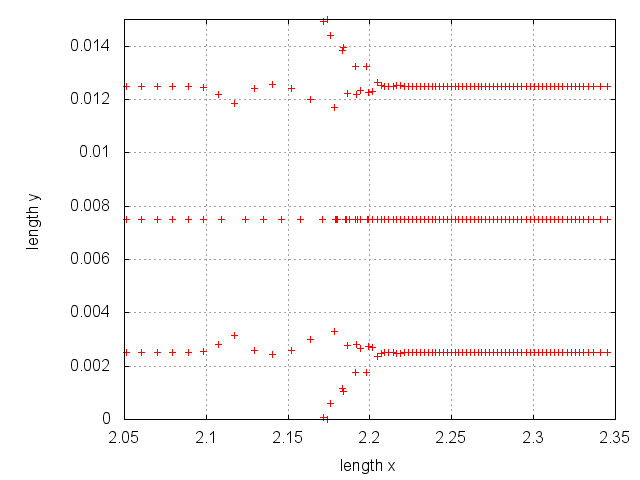
\includegraphics[width=7cm]{Graphics/results/ShockTube/q1D_CS_LF_SD/supLenVariat_dxdy005/Drifting/suplen015/x_y_plane00200653}}
\subfigure[supportlength 02]{
\label{fig:2DSPHresults_CS_drifting_suplen02}
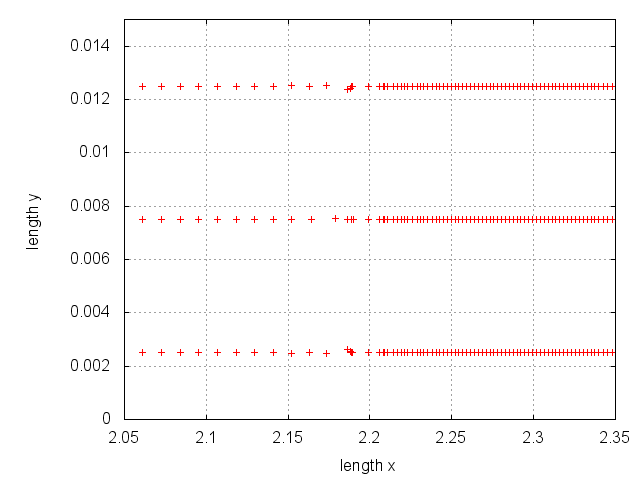
\includegraphics[width=7cm]{Graphics/results/ShockTube/q1D_CS_LF_SD/supLenVariat_dxdy005/Drifting/suplen02/x_y_plane00200841}}

\caption[particle drifting for 2D distribution]{particle drifting originating at the contact discontinuity for different support lengths}

\end{figure}

It is/are not only the particle positions that loose their perfect uniformity in the y- direction, but also the particle properties. This scattering is quantified by a variance calculation which shows results unequal zero in the contact discontinuity area.
Figure (\ref{fig:2DSPHresults_CS_variance}) shows exemplarily the variances of $\rho$ and $v$ along the shock--tube with significant amplitudes in the above mentionned area.

\begin{figure}[!htbp]
\centering
\label{fig:2DSPHresults_CS_variance}
\subfigure[supportlength 015]{
\label{fig:2DSPHresults_CS_variance_suplen015}
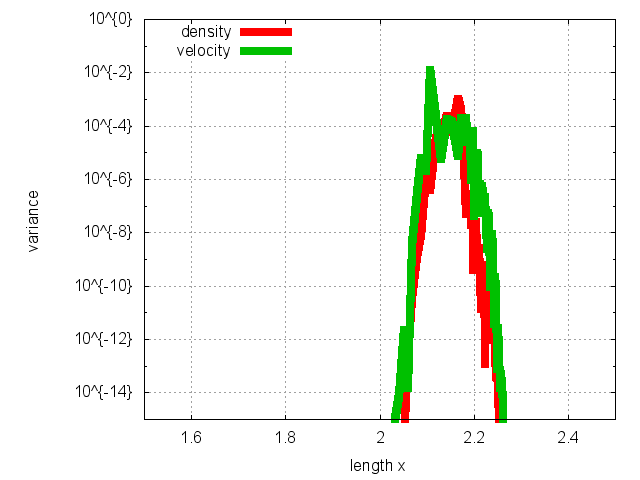
\includegraphics[width=7cm]{Graphics/results/ShockTube/q1D_CS_LF_SD/supLenVariat_dxdy005/Variance/suplen015/VarianceSupLen015}}
\subfigure[supportlength 02]{
\label{fig:2DSPHresults_CS_variance_suplen02}
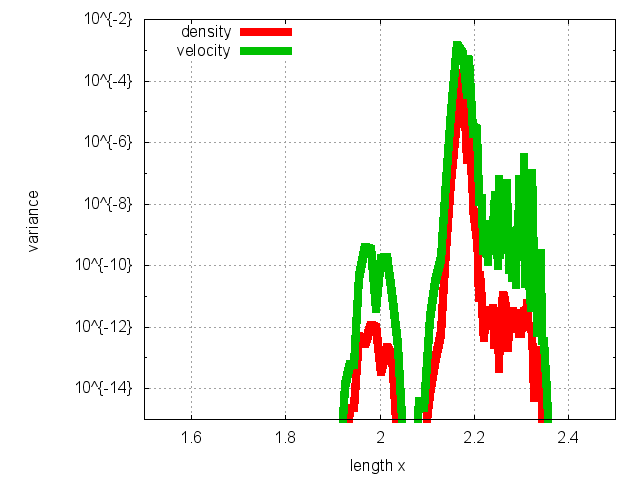
\includegraphics[width=7cm]{Graphics/results/ShockTube/q1D_CS_LF_SD/supLenVariat_dxdy005/Variance/suplen02/VarianceSupLen02}}

\caption[]{variance evolution along the shock--tube for the averaging of velocity and density at different supportlengths}

\end{figure}

The trend, that has been observed for the drifting, namely a decreasing effect with greater supportlength can roughly also be observed for the scattering of the x-position as well as all particle properties (figure (\ref{fig:2DSPHresults_CS_varianceVersusSuplen}).

\begin{figure}[!htbp]
\centering
\label{fig:2DSPHresults_CS_varianceVersusSuplen}
\subfigure[part 1]{
\label{fig:2DSPHresults_CS_varianceVersusSuplenPart1}
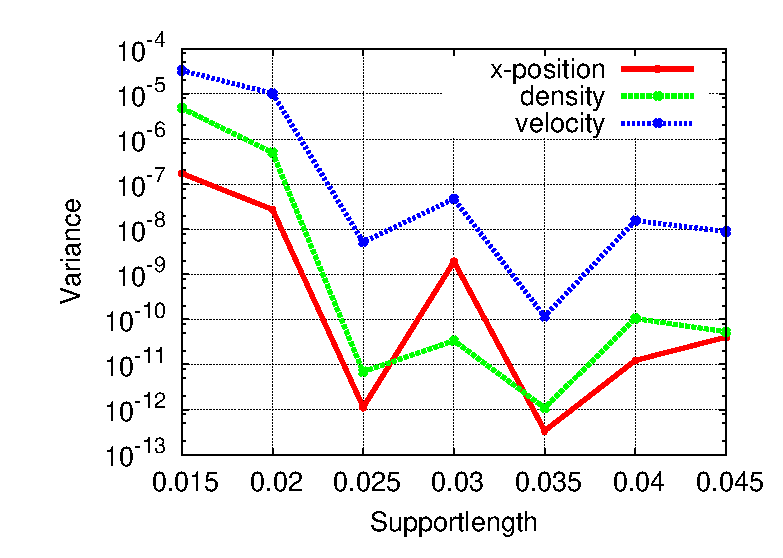
\includegraphics[width=7cm]{Graphics/results/ShockTube/q1D_CS_LF_SD/supLenVariat_dxdy005/Variance/VariancePart1}}
\subfigure[part 2]{
\label{fig:2DSPHresults_CS_varianceVersusSuplenPart2}
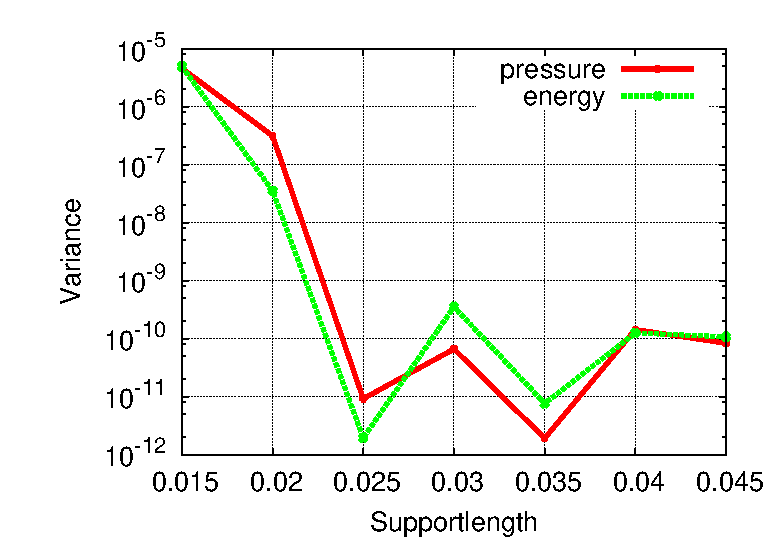
\includegraphics[width=7cm]{Graphics/results/ShockTube/q1D_CS_LF_SD/supLenVariat_dxdy005/Variance/VariancePart2}}

\caption[]{Evolution of variance with varying support length for all averaged quantities}

\end{figure}

This tendency of weakening with greater supportlength together with the fact that the particle drifting is symmetrical to the horizontal middle-line of the domain invokes the speculation that the non uniformity in the second direction might be caused by the peridoical boundary conditions in y-direction.


 
Despite of this change in properties in the second direction, the final results for the qD shock--tube problem, i.e. the averaged values, are very accurate and totally comparable to the corresponding simulation simulation with purely 1D particle distribution. Sometimes (but rarely) the averaged 2D results are even more accurate.
Nevertheless the 2D particle distribution leads to slightly greater oscillations in the velocity profile than for the comparable 1D distribution.
 

   
\paragraph{1D constant mass particle distribution}
For the following set of simulations, all particles, no matter if LHS or RHS of the shock tube, have the same mass of $m=0.001875$ which results in a spacing on the LHS of $dx_l=0.001875$ and $dx_r=0.015$ on the RHS to reproduce the initial density values. 
The globally optimum support length for this configuration is 0.025 (figure (\ref{fig:2DSPHresults_1D_CM_dx_const}), but even in this case small oscillations are already present in the velocity profile after the shock--front. These oscillations get quickly bigger with even smaller support length and simultaneously the accuracy of the after shock-values deteriorates considerably, which can be seen clearly in the error evolution in area 3 in figure (\ref{fig:2DSPHresults_1D_CM_dx_const}). 
This is due to the insufficient number of neighbouring particles in the RHS of the shock tube, where the particle distance is eight times higher than in the LHS. For a supportlength of 0.02 there are barely 2 neighbouring particles which contribute to the interpolation on the RHS and for a supportlength of 0.015 there is just no neighbour any more and the interpolation is limited to the proper contribution of the particle itself, which is of course erroneous. 

The inaccuracy in the rarefaction, which was encountered for a constant spacing particle distributions both in 1D and 2D (see e.g. figure (\ref{figureBeiDT})) does not develop in the case of a 1D constant mass particle distribution. This might be the reason why 
in literature SPH shock--tube simulations are mostly found using the constant mass initialization approach \cite{Monaghan1983,Monaghan2005,Liu2003}, which also seems the physically more logical one.

For an example for the profiles of $\rho, p, u, e$ refer to figure (\ref{fig:1DSPHresults}) in the result section of the 1D code. 



\begin{figure}[H]
\centering
\label{fig:2DSPHresults_1D_CM_dx_const}

\subfigure[tight][whole domain]{
\label{fig:2DSPHresults_1D_CM_dx_const_wholeRho}
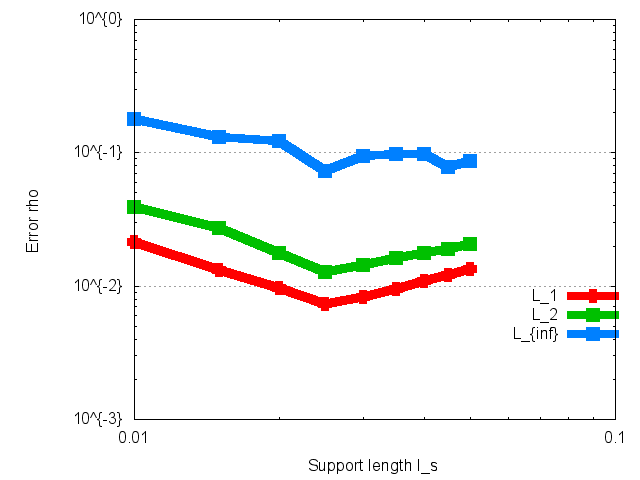
\includegraphics[width=5cm]{Graphics/results/ShockTube/1D_CM_LF_SD/supLenVariat_m001875/WholeDomainRho}}
\subfigure[tight][whole domain]{
\label{fig:2DSPHresults_1D_CM_dx_const_3Rho}
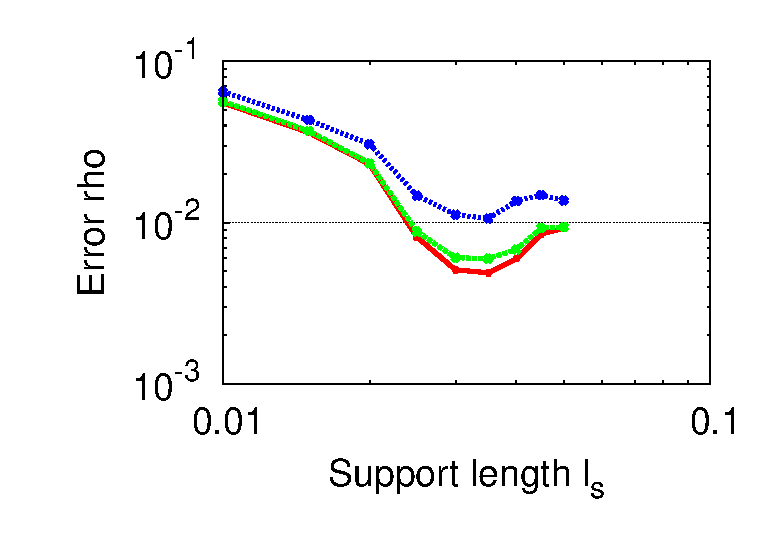
\includegraphics[width=5cm]{Graphics/results/ShockTube/1D_CM_LF_SD/supLenVariat_m001875/Area3Rho}}
\subfigure[tight][whole domain]{
\label{fig:2DSPHresults_1D_CM_dx_const_2Rho}
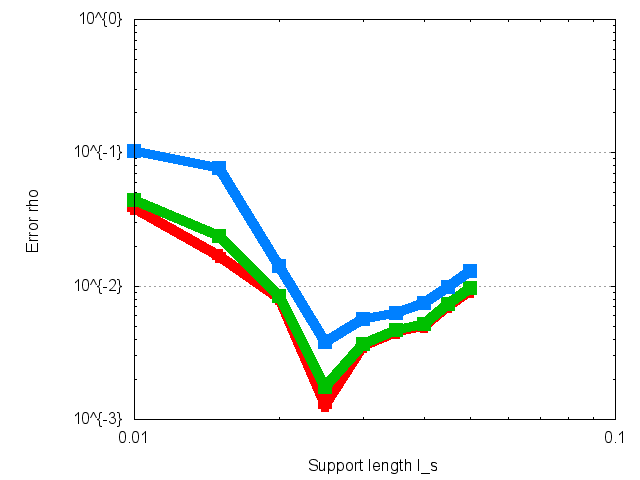
\includegraphics[width=5cm]{Graphics/results/ShockTube/1D_CM_LF_SD/supLenVariat_m001875/Area2Rho}}
\subfigure[tight][area 3]{
\label{fig:2DSPHresults_1D_CM_dx_const_wholeU}
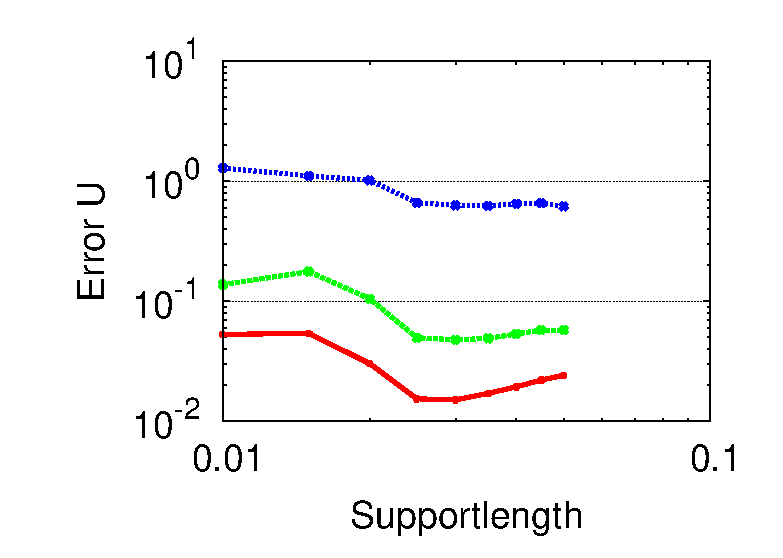
\includegraphics[width=5cm]{Graphics/results/ShockTube/1D_CM_LF_SD/supLenVariat_m001875/WholeDomainU}}
\subfigure[tight][area 3]{
\label{fig:2DSPHresults_1D_CM_dx_const_3U}
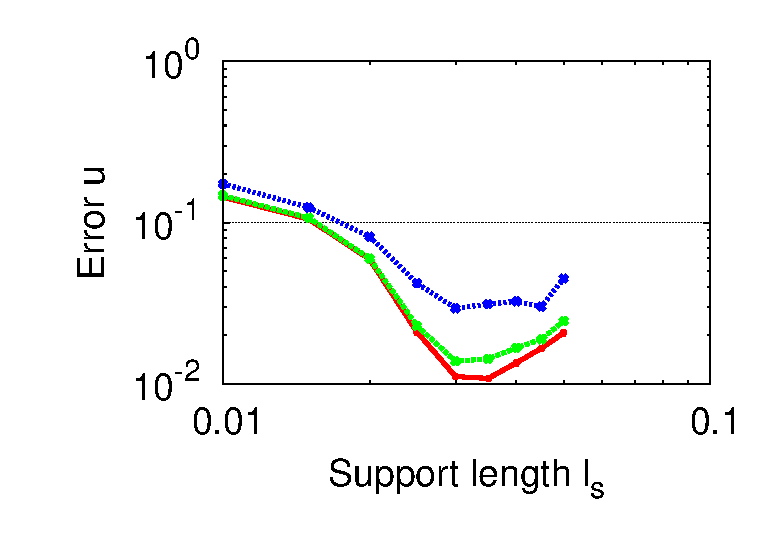
\includegraphics[width=5cm]{Graphics/results/ShockTube/1D_CM_LF_SD/supLenVariat_m001875/Area3U}}
\subfigure[tight][area 3]{
\label{fig:2DSPHresults_1D_CM_dx_const_2U}
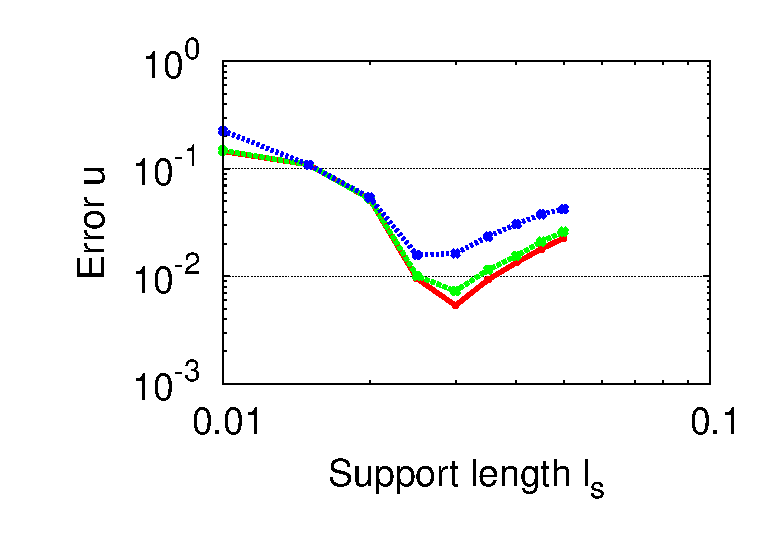
\includegraphics[width=5cm]{Graphics/results/ShockTube/1D_CM_LF_SD/supLenVariat_m001875/Area2U}}
\subfigure[tight][area 2]{
\label{fig:2DSPHresults_1D_CM_dx_const_wholeE}
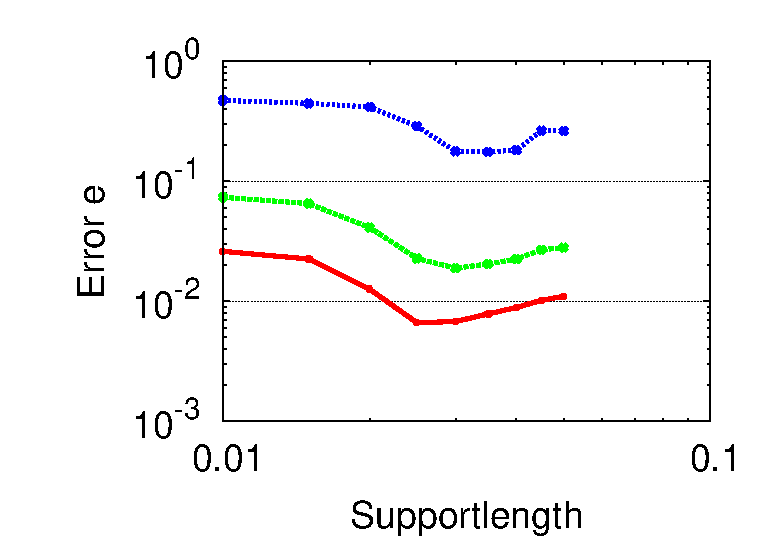
\includegraphics[width=5cm]{Graphics/results/ShockTube/1D_CM_LF_SD/supLenVariat_m001875/WholeDomainE}}
\subfigure[tight][area 2]{
\label{fig:2DSPHresults_1D_CM_dx_const_3E}
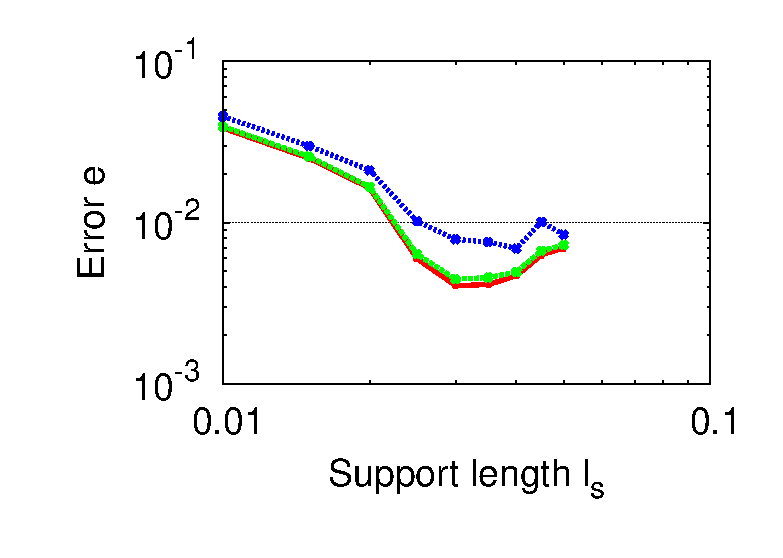
\includegraphics[width=5cm]{Graphics/results/ShockTube/1D_CM_LF_SD/supLenVariat_m001875/Area3E}}
\subfigure[tight][area 2]{
\label{fig:2DSPHresults_1D_CM_dx_const_2E}
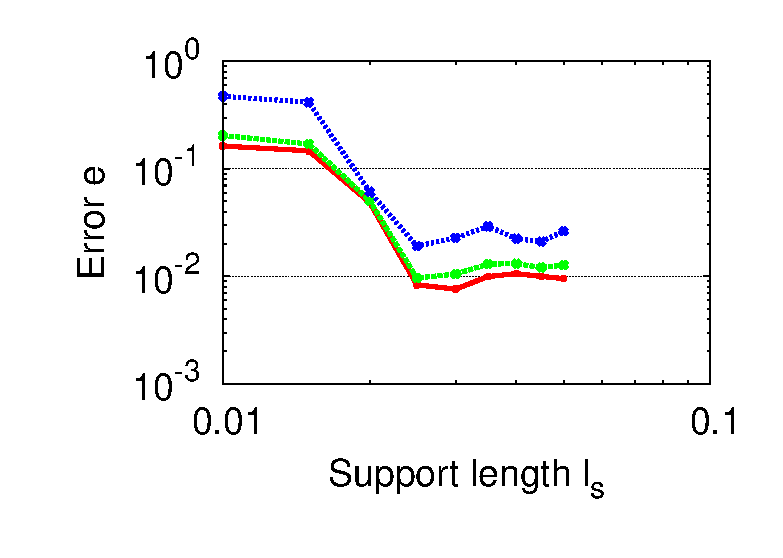
\includegraphics[width=5cm]{Graphics/results/ShockTube/1D_CM_LF_SD/supLenVariat_m001875/Area2E}}

\caption[Convergence Shock-tube with 1D constant mass particle distribution]{L--norm errors of $\rho, u, e$ for a series of simulation with a varying supoprt length and a constant particle spacing mass of $m=0.001875$ leading to a spacing on the LHS of $dx_l=0.001875$ and $dx_r=0.015$ on the RHS. The simulation is evaluated at $t=0.2$}

\end{figure}

\paragraph{2D constant mass particle distribution}
The employed particle mass $m=2.5e-5$ corresponds to a spacing of $dx_l=dy_l=0.005$ on the LHS and of $dx_r=dy_r=0.015$ on the RHS.
Simlations with this 2D constant mass marticle distribution give the best results for a support length of 0.03. However due to the discontiutity of the particle distribution in y direction at the interface, there is a very weak drifting of the interface particles on the high density side in y direction. This phenomenon increases with smaller supportlength - a tendency that has already been observed for the 2D constant spacing particle initialization. 
Besides, for most of the simulated cases there is again an inaccuracy in the velocity profile  within the rarefaction wave. The same has already been observed for 1D and 2D constant spacing initializations but not for 1D constant mass initializations.
The mentionned inaccuracy only disappeares for supportlenghts $\geq0.4$.

The error evolution for the above discussed set of simulations can be found in the appendix, as there is no remarkable difference to the ones already shown. Due to the appearing inaccuracy in the rarefaction the figures look more like the ones from the constant spacing initialization than the one for 1D constant mass. 



\subsubsection{Resolution Study - ratio smoothinglength/spacing held constant}
In this section, the resolution is gradually increased by simultaneously diminuishing both the supportlength and the particle spacing in a way that their ratio remains constant. This means that the number of nearest neighbour particles remains constant. 
The convergence towards the exact solution is tested and the convergence ratio for each of the above mentionned four cases is determined. Having determined an optimum ratio of supportlength to particle spacing above, it is used here to obtain the highest possible accuracy for the simulation. In another set of simulations, at least for the purely 1D particle distributions, a non-optimum ratio is employed to verify the robustness of the method (kann man das sagen, ist das Robustness verification? Gibt es in der Numerik eine eigene, spezielle Definition von Robustness).

\paragraph{1D constant spacing particle distribution}
The simulations are conducted for a ratio of supportlength to particle spacing of 5 and the resolution is increased from a supportlength of 0.025 to 0.005, which corresponds to a number of particles from $N=401$ to $N02001$. 
Figure (\ref{fig:2DSPHresults_1D_CS_ratioConst}) shows the quantitative evaluation of this set of simulation by means of the L-norm errors. The $L_1$ error shows roughly a first order convergence for all investigated quantities $\rho, u, e$ in all areas whereas the $L_2$ convergence is slightly lower.  (WARUM?)
The $L_{\inf}$ error of all quantities in the global domain are constant and caused by the non-discontinuous shock-resolution.

By the way, the inaccuracy in the rarefaction already encountered in section (\ref{sec:2DSPH_results_shock_resSTudy_dx=const}) n for constant spacing particle distribution does not disappear but remains of about the same size, even for the highest resolution. 

Außerdem, wie war das mit der Konvergenz? bei h/dx=const, convergierts dann gegen 0 oder bleibt ein resideller Fehler wegen Disktretisierungseffekt (dx). Müsste doch davon abhängen, on Diskretisierungsfehler von (h/dx) oder dx absolut abhängt!

ERWÄHNEN WIE DIE KONVERGENZ FÜR ANDERE RATIO h/dx IST!!! (noch machen)!
 

\begin{figure}[H]
\centering
\label{fig:2DSPHresults_1D_CS_ratioConst}

\subfigure[tight][whole domain]{
\label{fig:2DSPHresults_1D_CS_ratioConst_wholeRho}
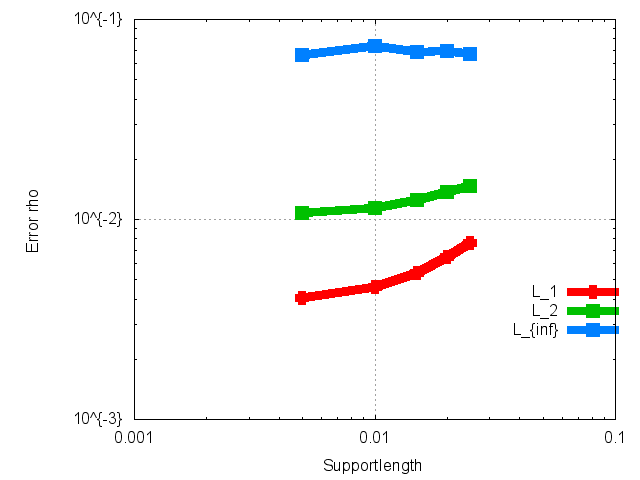
\includegraphics[width=5cm]{Graphics/results/ShockTube/1D_CS_LF_SD/ratio_supLenDx5_dt0025/autom_dt_control/WholeDomainRho}}
\subfigure[tight][whole domain]{
\label{fig:2DSPHresults_1D_CS_ratioConst_3Rho}
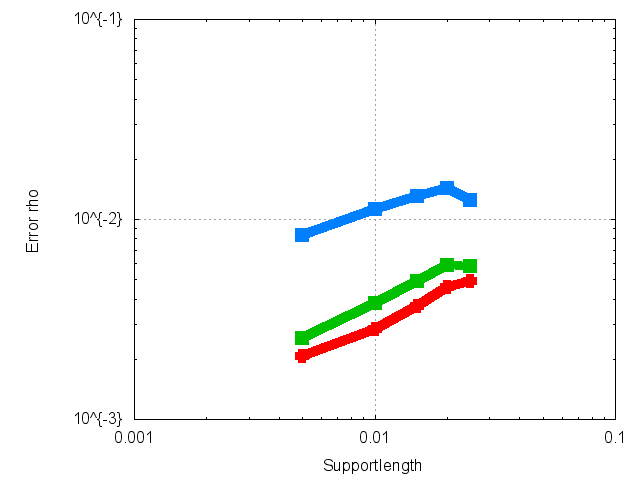
\includegraphics[width=5cm]{Graphics/results/ShockTube/1D_CS_LF_SD/ratio_supLenDx5_dt0025/autom_dt_control/Area3Rho}}
\subfigure[tight][whole domain]{
\label{fig:2DSPHresults_1D_CS_ratioConst_2Rho}
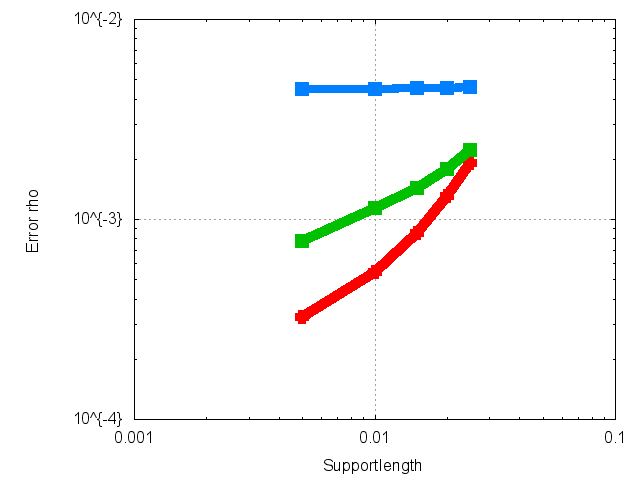
\includegraphics[width=5cm]{Graphics/results/ShockTube/1D_CS_LF_SD/ratio_supLenDx5_dt0025/autom_dt_control/Area2Rho}}
\subfigure[tight][area 3]{
\label{fig:2DSPHresults_1D_CS_ratioConst_wholeU}
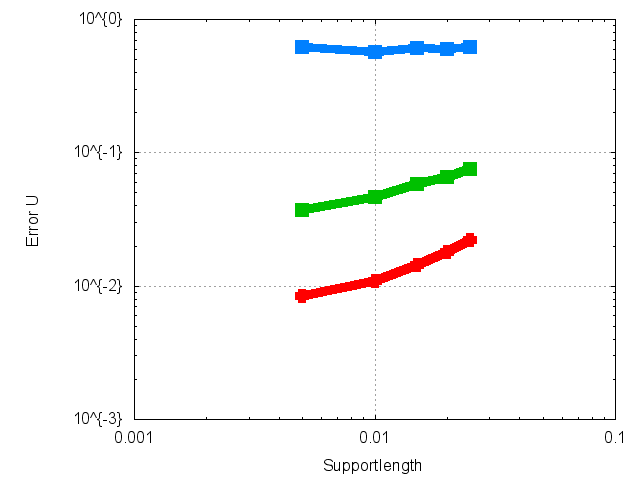
\includegraphics[width=5cm]{Graphics/results/ShockTube/1D_CS_LF_SD/ratio_supLenDx5_dt0025/autom_dt_control/WholeDomainU}}
\subfigure[tight][area 3]{
\label{fig:2DSPHresults_1D_CS_ratioConst_3U}
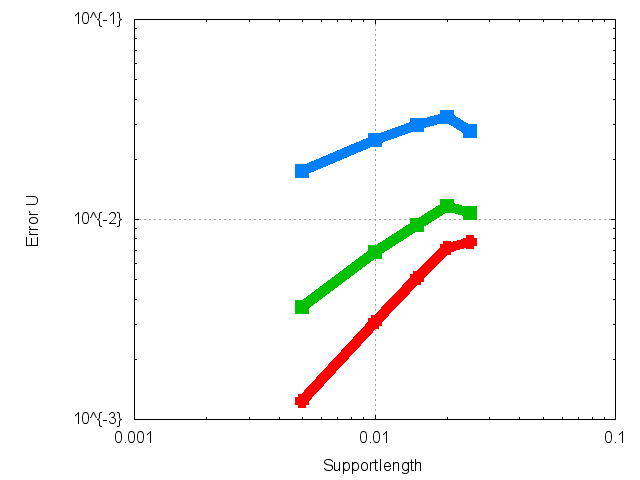
\includegraphics[width=5cm]{Graphics/results/ShockTube/1D_CS_LF_SD/ratio_supLenDx5_dt0025/autom_dt_control/Area3U}}
\subfigure[tight][area 3]{
\label{fig:2DSPHresults_1D_CS_ratioConst_2U}
\includegraphics[width=5cm]{Graphics/results/ShockTube/1D_CS_LF_SD/ratio_supLenDx5_dt0025/autom_dt_control/Area2U}}
\subfigure[tight][area 2]{
\label{fig:2DSPHresults_1D_CS_ratioConst_wholeE}
\includegraphics[width=5cm]{Graphics/results/ShockTube/1D_CS_LF_SD/ratio_supLenDx5_dt0025/autom_dt_control/WholeDomainE}}
\subfigure[tight][area 2]{
\label{fig:2DSPHresults_1D_CS_ratioConst_3E}
\includegraphics[width=5cm]{Graphics/results/ShockTube/1D_CS_LF_SD/ratio_supLenDx5_dt0025/autom_dt_control/Area3E}}
\subfigure[tight][area 2]{
\label{fig:2DSPHresults_1D_CS_ratioConst_2E}
\includegraphics[width=5cm]{Graphics/results/ShockTube/1D_CS_LF_SD/ratio_supLenDx5_dt0025/autom_dt_control/Area2E}}

\caption[Convergence Shock-tube 1D constant spacing particle distribution]{L--norm errors of $\rho, u, e$ for a series of simulation with increasing resolution and a constant ratio of support length to spacing of 5 evaluated at $t=0.2$}

\end{figure}

\paragraph{2D constant spacing particle distribution}
Exactly like the corresponding 1D particle distribution, the 2D distribution showed optimum results for a ratio $h/dx=2.5$ (supportlength/dx=5, muss mir noch ne Abkürzung für supportlength einfallen lassen, damit ich sie nicht immer ausschreiben muss, evtl $l_s$???) which is also taken for this set of simulations. The supportlength variation ranges from 0.025 to 0.005 which leads to a number of particles from $N=1995$ for the lowest resolution to $N=9995$ for the highest simulation. As for higher resolution not only the number of particles becomes higher but also the timestep, which is coupled to $h$, becomes smaller, the time needed for the simulation increases considerably. (2h30 on my (old) computer for the highest resolution case)

The convergence behaviour for this case of a 2D particle distribution with constant spacing is essentially the same as for the corresponding 1D case. i.e. about first order convergence. Therefore the graphical evaluation of the results is presented in the appendix.

In section (\ref{sec:2DSPH_results_shock_resSTudy_dx=const}), it has turned out that the 2D particle distribution result shows more velocity-oscillations in the aftershock area than one obtained with a 1D distribution. While these osciallations vanish for the 1D distribution with increasing resolution, they remain clearly visible in the velocity profile for the 2D distribution, even at the highest simualated resolution. They just become more and more confined to the area directly after the shock and at the contact discontinuity. 

 
\paragraph{1D constant mass particle distribution}
For the convergence test of the 1D constant mass particel distribution, a constant ratio $l_s/m=16$ has been taken, leading to ratios of $l_s/dx_l=$ on the LHS and $l_s/dx_r=$ on the RHS of the shock-tube problem. Again, the convergence rate is about first order as already for all cases before. The corresponding figure is shown in the Appendix. 

At the highest simulated resolution with $l_s=0.005$, corresponding to 3599 particles, the simulation result has a good quality. The shock is resolved very well, as its resolution scales with $l_s$ and the aftershock values are matched very accurately.

VIELLEICHT NOCHMAL DIE 4 BILDER VON EINER HOCHAUFLÖSENDEN SCHOCK-SIMULATION (WÄRE ABER ÄHNLICH ZU 1DSPH!!!)

AUẞERDEM KONVERGENZTEST NOCH FÜR NICHT-OPTIMALE RATIO SUPlEN/DX...->ROBUSTNESS


\paragraph{2D constant mass particle distribution}
Finally, the convergence of a 2D constant mass particle distribution has been examined using a constant ratio $l_s/\sqrt{m}=6$ found to be optimal in section (\ref{sec:2DSPH_results_shock_resSTudy_dx=const}) and a variation of $l_s$ from 0.3 to 0.1, corresponding to 3994 particles in the highest resolution.
The obtained convergence ratio is again around 1 order as can be seen from the figure in the Appendix. 

The inaccuracy in the rarefaction that has been observed in section (\ref{sec:2DSPH_results_shock_resSTudy_dx=const}) for a 2D constant mass particle distribution does not disappear with higher resolution. 
%vielleicht noch erwähnen dass eine weitere simulation durchgeführt wurde mit relativ größerer supLen (in Anlehnung an Resultate von 1D const mass distribution). i.e. ratio suplen/sqrt(m)=8 with supLen=0.01: Ergebnis: fehler in der rarefaktion ist weg! 
 

\subsubsection{Perturbation Study}
\paragraph{1D constant spacing particle distribution}
\begin{figure}[H]
\centering
\label{fig:2DSPHresults_1D_CS_ratioConst}

\subfigure[tight][whole domain]{
\label{fig:2DSPHresults_1D_CS_ratioConst_wholeRho}
\includegraphics[width=5cm]{Graphics/results/ShockTube/PertStudy/basedOn1DconstSpace/WholeDomainRho}}
\subfigure[tight][whole domain]{
\label{fig:2DSPHresults_1D_CS_ratioConst_3Rho}
\includegraphics[width=5cm]{Graphics/results/ShockTube/PertStudy/basedOn1DconstSpace/Area3Rho}}
\subfigure[tight][whole domain]{
\label{fig:2DSPHresults_1D_CS_ratioConst_2Rho}
\includegraphics[width=5cm]{Graphics/results/ShockTube/PertStudy/basedOn1DconstSpace/Area2Rho}}
\subfigure[tight][area 3]{
\label{fig:2DSPHresults_1D_CS_ratioConst_wholeU}
\includegraphics[width=5cm]{Graphics/results/ShockTube/PertStudy/basedOn1DconstSpace/WholeDomainU}}
\subfigure[tight][area 3]{
\label{fig:2DSPHresults_1D_CS_ratioConst_3U}
\includegraphics[width=5cm]{Graphics/results/ShockTube/PertStudy/basedOn1DconstSpace/Area3U}}
\subfigure[tight][area 3]{
\label{fig:2DSPHresults_1D_CS_ratioConst_2U}
\includegraphics[width=5cm]{Graphics/results/ShockTube/PertStudy/basedOn1DconstSpace/Area2U}}
\subfigure[tight][area 2]{
\label{fig:2DSPHresults_1D_CS_ratioConst_wholeE}
\includegraphics[width=5cm]{Graphics/results/ShockTube/PertStudy/basedOn1DconstSpace/WholeDomainE}}
\subfigure[tight][area 2]{
\label{fig:2DSPHresults_1D_CS_ratioConst_3E}
\includegraphics[width=5cm]{Graphics/results/ShockTube/PertStudy/basedOn1DconstSpace/Area3E}}
\subfigure[tight][area 2]{
\label{fig:2DSPHresults_1D_CS_ratioConst_2E}
\includegraphics[width=5cm]{Graphics/results/ShockTube/PertStudy/basedOn1DconstSpace/Area2E}}

\caption[Perturbation influence shock-tube with 1D constant spacing particle distribution]{L--norm errors of $\rho, u, e$ for a series of simulation with increasing perturbation of initial particle position}

\end{figure}


\paragraph{2D constant spacing particle distribution}
\begin{figure}[H]
\centering
\label{fig:2DSPHresults_1D_CS_ratioConst}

\subfigure[tight][whole domain]{
\label{fig:2DSPHresults_1D_CS_ratioConst_wholeRho}
\includegraphics[width=5cm]{Graphics/results/ShockTube/PertStudy/basedOn2DConstSpaceContDensity/WholeDomainRho}}
\subfigure[tight][whole domain]{
\label{fig:2DSPHresults_1D_CS_ratioConst_3Rho}
\includegraphics[width=5cm]{Graphics/results/ShockTube/PertStudy/basedOn2DConstSpaceContDensity/Area3Rho}}
\subfigure[tight][whole domain]{
\label{fig:2DSPHresults_1D_CS_ratioConst_2Rho}
\includegraphics[width=5cm]{Graphics/results/ShockTube/PertStudy/basedOn2DConstSpaceContDensity/Area2Rho}}
\subfigure[tight][area 3]{
\label{fig:2DSPHresults_1D_CS_ratioConst_wholeU}
\includegraphics[width=5cm]{Graphics/results/ShockTube/PertStudy/basedOn2DConstSpaceContDensity/WholeDomainU}}
\subfigure[tight][area 3]{
\label{fig:2DSPHresults_1D_CS_ratioConst_3U}
\includegraphics[width=5cm]{Graphics/results/ShockTube/PertStudy/basedOn2DConstSpaceContDensity/Area3U}}
\subfigure[tight][area 3]{
\label{fig:2DSPHresults_1D_CS_ratioConst_2U}
\includegraphics[width=5cm]{Graphics/results/ShockTube/PertStudy/basedOn2DConstSpaceContDensity/Area2U}}
\subfigure[tight][area 2]{
\label{fig:2DSPHresults_1D_CS_ratioConst_wholeE}
\includegraphics[width=5cm]{Graphics/results/ShockTube/PertStudy/basedOn2DConstSpaceContDensity/WholeDomainE}}
\subfigure[tight][area 2]{
\label{fig:2DSPHresults_1D_CS_ratioConst_3E}
\includegraphics[width=5cm]{Graphics/results/ShockTube/PertStudy/basedOn2DConstSpaceContDensity/Area3E}}
\subfigure[tight][area 2]{
\label{fig:2DSPHresults_1D_CS_ratioConst_2E}
\includegraphics[width=5cm]{Graphics/results/ShockTube/PertStudy/basedOn2DConstSpaceContDensity/Area2E}}

\caption[Perturbation influence shock-tube with 1D constant spacing particle distribution]{L--norm errors of $\rho, u, e$ for a series of simulation with increasing perturbation of initial particle position}

\end{figure}
\paragraph{1D constant mass particle distribution}
\begin{figure}[H]
\centering
\label{fig:2DSPHresults_1D_CS_ratioConst}

\subfigure[tight][whole domain]{
\label{fig:2DSPHresults_1D_CS_ratioConst_wholeRho}
\includegraphics[width=5cm]{Graphics/results/ShockTube/PertStudy/basedOn1DconstMass/WholeDomainRho}}
\subfigure[tight][whole domain]{
\label{fig:2DSPHresults_1D_CS_ratioConst_3Rho}
\includegraphics[width=5cm]{Graphics/results/ShockTube/PertStudy/basedOn1DconstMass/Area3Rho}}
\subfigure[tight][whole domain]{
\label{fig:2DSPHresults_1D_CS_ratioConst_2Rho}
\includegraphics[width=5cm]{Graphics/results/ShockTube/PertStudy/basedOn1DconstMass/Area2Rho}}
\subfigure[tight][area 3]{
\label{fig:2DSPHresults_1D_CS_ratioConst_wholeU}
\includegraphics[width=5cm]{Graphics/results/ShockTube/PertStudy/basedOn1DconstMass/WholeDomainU}}
\subfigure[tight][area 3]{
\label{fig:2DSPHresults_1D_CS_ratioConst_3U}
\includegraphics[width=5cm]{Graphics/results/ShockTube/PertStudy/basedOn1DconstMass/Area3U}}
\subfigure[tight][area 3]{
\label{fig:2DSPHresults_1D_CS_ratioConst_2U}
\includegraphics[width=5cm]{Graphics/results/ShockTube/PertStudy/basedOn1DconstMass/Area2U}}
\subfigure[tight][area 2]{
\label{fig:2DSPHresults_1D_CS_ratioConst_wholeE}
\includegraphics[width=5cm]{Graphics/results/ShockTube/PertStudy/basedOn1DconstMass/WholeDomainE}}
\subfigure[tight][area 2]{
\label{fig:2DSPHresults_1D_CS_ratioConst_3E}
\includegraphics[width=5cm]{Graphics/results/ShockTube/PertStudy/basedOn1DconstMass/Area3E}}
\subfigure[tight][area 2]{
\label{fig:2DSPHresults_1D_CS_ratioConst_2E}
\includegraphics[width=5cm]{Graphics/results/ShockTube/PertStudy/basedOn1DconstMass/Area2E}}

\caption[Perturbation influence shock-tube with 1D constant mass particle distribution]{L--norm errors of $\rho, u, e$ for a series of simulation with increasing perturbation of initial particle position}

\end{figure}

\paragraph{2D constant mass particle distribution}
DONE -- NOT YET INTEGRATED IN REPORT
\subsection{linear acoustic waves}

DONE -- NOT YET INTEGRATED IN REPORT
%..\cite{Monaghan1992}: good agreement with theory if wavelength $\lambda > 2\pi h$. Besides better results (particularly in terms of propagation speed), if $\Delta x=1$ or $\Delta x=2$ than with $\Delta x=1.5$


\subsection{Taylor--Green flow}
ALMOST DONE -- NOT YET INTEGRATED IN REPORT

\subsection{Pure Heat--Conduction}
DONE -- NOT YET INTEGRATED IN REPORT
\subsubsection{Verification of timestep--condition for conduction}
Noch überlegen in welche sub oder subsub section dieser Schritt kommt.
Denn eigentlich gehört er unter adiabatic slab, da dies die simulierte Konfiguration ist, allerdings ist die Verifikation allgemeingültig gedaxht, d.h auch z.b für isothermal slab. Dies würde dafür sprechen, ein extra kapitel aufzumachen. Und zwar am Anfang von Heatconduction wäre am logischsten (da bevor eigentlich simuliert wird, dt getestet werden müsste müsste...)

Based on the 40x20 particle distribution and adiabatic BC, the correctness of the
heat conduction-related timestepping criterion expressed in equation (REFERENCE) ist tested. The simulation errors, conducted with different timesteps, are compared at a simulation time of 1 sec. (although the error (due to spatial discretization) is max. at much smaller times). 
EVTL. RESOLUTION STUDY DESWEGEN NCIHMAL MACHEN UND ZWAR FÜR JEDE SUPLEN MIT IHREM OPTIMALEN TIMESTEP! VIELLECIHT ERKLÄRT DISEE TATSACHE DASS DIE KONVERENZ NICHT SO ``GLATT'' IST...


\begin{figure}[h]  
  \label{fig:PureHeat_dtVerification}
  \centering
  \includegraphics[width=0.95\textwidth]{Graphics/results/PureHeatConduction/ErrorTimestep}
  \caption{Evolution of the error after at $t=1.25$ with a variation of timestep}
\end{figure}

Figure \ref{fig:PureHeat_dtVerification}: there is a real optimum, i.e. slight deterioration of the results when $dt<dt_{mathit{opt}}$!!! According to \cite{Cleary1999}, more details on timestepping for a pure conduction problem can be found in \cite{} (could not access article yet).
(somehow strange that results get worse if dt diminuishes???, does this have to do with the initial discontinuity or is this a normal behaviour?????)
Problems also for flow simulation, when several timestepping criteria apply and in general dt < (sometimes even dt<<) dt opt for heat conduction! Have a look at literature (e.g. Cleary2002, where the heat conduction model is applied to flows).

\subsubsection{Slab with temperature jump and adiabatic boundary conditions}


\begin{figure}[!htbp]
\centering
\label{fig:PureHeat_T_profilesInitialPhase}
\subfigure[at $t=0.1$]{
\label{fig:PureHeat_T_profilesInitialPhase0.1}
\includegraphics[width=5.7cm,height=5cm]{Graphics/results/PureHeatConduction/T_profiles000000100000}}
\subfigure[at $t=1.0$]{
\label{fig:PureHeat_T_profilesInitialPhase1}
\includegraphics[width=5.7cm,height=5cm]{Graphics/results/PureHeatConduction/T_profiles000001000000}}
\subfigure[at $t=2.0$]{
\label{fig:PureHeat_T_profilesInitialPhase2}
\includegraphics[width=5.7cm,height=5cm]{Graphics/results/PureHeatConduction/T_profiles000002000000}}
\subfigure[at $t=4.0$]{
\label{fig:PureHeat_T_profilesInitialPhase4}
\includegraphics[width=5.7cm,height=5cm]{Graphics/results/PureHeatConduction/T_profiles000003999999}}

\caption[Temperature profiles at the initial phase of equalization]{Temperature profiles for the slab-with-T-jump testcase (find REFERENCE in paragraph where test cases are described) Npart 40x20 }

\end{figure}




\begin{figure}[h]  
  \label{fig:PureHeat_temporalErrorEvolution}
  \centering
  \includegraphics[width=0.95\textwidth]{Graphics/results/PureHeatConduction/temporalErrEvolution}
  \caption{temporal evolution of the L-morm errors for the initial phase (as long as alanytical reference solution is valid}
\end{figure}

(\ref{fig:temporalErrorEvolution}) geht nur bis 4sek, da danach bereits der Fehler, der dadurhc gemacht wird, die analytissche Lsg. des haöbunendlichen Körpers zu nehmen, dominiert.! (siehe entsprechende README, wo das vorgerechnet ist...)
The errors are biggest short after the beginning of the simulation due to the discontinuity in temperature \cite{Cleary1999}. But as soon as the discontinuity gets smoothed by the thermal conduction, the results become very accurate.

Spacial accuracy and convergence of this SPH heat conduction model have been extensively demonstrated by \cite{Cleary1999}.Only a short verification is given with figure (\ref{fig:PureHeat_ErrorResolution}), where the evolution of the L-nor errors with the spacial resolution is traced. The errors are evaluated short after the beginning of the simulation, as they are biggest there (see figure (\ref{fig:PureHeat_temporalErrorEvolution} 

facts for resolution study (probably to be put in paragraph above which describes simu-setup): variation of Nx, (h (h=dx, or suplen02dx) is varied in a way that number of neighbors stay constant, i.e. h/dx=const., 
for Ny the following applies: the spacing dy is always kept=dx. The simulation domain which originally has the dimensions 1x0.5 however, is changed in y direction in order to host only entire cells (these have size of supLen).
But this is not a problem and does not influence the results at all, as the BC in y direction is periodic and the problem is actually 1D!
The ``new'' domain-size has to be taken into account for the initial particle generation. I choose domainsizey=cellsize(=supLen) for minimum calculation effort.
dt is manually choesen in a way that 0.1 its a multiple, dt<dtautom!




Another interesting finding of \cite{Cleary1999} is, that adiabatic boundary conditions influence heat conduction tangential to the boundary. This is not important here, but has to be kept in mind for further applicatons.




\begin{figure}[h]  
  \label{fig:PureHeat_EnergyEvolution}
  \centering
  \includegraphics[width=0.95\textwidth]{Graphics/results/PureHeatConduction/EnergyContentEvolution}
  \caption{Evolution of the energy content (see equation (\ref{eq:energyContent})) in the adiabatic slab, (simulation with 40x 20 particles), energy content calculated every time unit}
\end{figure}

\begin{figure}[h]  
  \label{fig:PureHeat_TProfile}
  \centering
  \includegraphics[width=0.95\textwidth]{Graphics/results/PureHeatConduction/T_profile000650062499}
  \caption{Temperature profile at around 650 time units}
\end{figure}
\ref{fig:PureHeat_TProfile} shows the temperature profile in the adiabatic slab 
after a long simulation time and very close to the entire equalization. The pofile is symmetric arount the center of the slab, as one would expect given thie initial condition. Furthermore, the temperature profile is perfectly horizontal at the edges, which is in agreement with the imposed adiabatic boundary condtion.

convergence study

\begin{figure}[h]  
  \label{fig:PureHeat_ErrorResolution}
  \centering
  \includegraphics[width=0.95\textwidth]{Graphics/results/PureHeatConduction/ErrorResolution}
  \caption{Evolution of the L-norm errors with variation of spatial resoultion}
\end{figure}
Figure (\ref{fig:PureHeat_ErrorResolution})




\subsubsection{Slab with temperature jump and isothermal boundary conditions}

\begin{figure}[!htbp]
\centering
\label{fig:PureHeat_Isothermal}
\subfigure[at $t=2.0$]{
\label{fig:PureHeat_Isothermal_t2}
\includegraphics[width=5.7cm,height=5cm]{Graphics/results/PureHeatConduction/isothermal/T_profile000002000000}}
\subfigure[at $t=200.0$]{
\label{fig:PureHeat__Isothermal_t200}
\includegraphics[width=5.7cm,height=5cm]{Graphics/results/PureHeatConduction/isothermal/T_profile000200000000}}

\caption[Temperature profiles for slab with isothermal edges]{Temperature profiles for slab with isothermal boundary conditions \subref{fig:PureHeat_Isothermal_t2} in the initial phase and \subref{fig:PureHeat_Isothermal_t200} after a steady-state solution has established}

\end{figure}

..the fact that the temperature profile does not exactly pass through 0 and 1 at the corresponding edges is not an implementation fault, but is linked to the particle initialization. For the above case the first real particles are placed at half a particle distance from the domain edges. As the boundary particles for the wall and free slip boundary conditions are placed by mirroring at the domain edge, the closest boundary particle to the edge is also located $\Delta x/2$ away from it. This means that effectively in this case, the constant temperature is not forced directly at the domain edge but only $\Delta x/2$ away. Comparison with figure (REF) confirms this. If one wanted to place the effective boundary exactly at the nominal domain edge, one would have to adapt the initial particle placement in a way that the first mirrored particle coincides with the domain edge (may perhaps cause problems because then, there are two particles at the very domain edge: one real and one boundary particle). Other solution: define the nominal calculation domain a bit smaller so that the effective calculation domain coincides with the desired one (this does only work for pure heat conduction, as for flow problems, the effective (kinematic) domain edge always coincides with the nominal one ...)

Order of convergence reduced with implementation of isothermal boundaries from second to first order \cite{Cleary1999}

\subsection{Compressible Couette--flow}
STILL TO BE DONE


\begin{comment}
In the Figure~\ref{fig:1dshock} one can see \ldots

\begin{figure}[h]
  \centering
  \includegraphics[width=0.95\textwidth]{img/1dshock.eps}
  \caption{An example of a figure}
  \label{fig:1dshock}
\end{figure}

\end{comment}

\chapter{Conclusion}
\label{sec:conclusion}
As the project is not finished until december, it may be to early to draw a final conclusion. However, I am optimistic to be able to simulate a configuration including porosities by the end of the project. I used the time so far to become familiarized with the SPH--method and all the tools that go with an activity in numerics (including Linux and Co.). As a first step I developed a little 1D SPH--code. Then I tried to understand the 2D incompressible multiphase SPH code, which I had to modify. This accomplished, I started implementing the equations which I had identified with the little 1D code as the right ones for compressible flows and adapted the 2D code to that effect. The shock--tube test case and the acoustic wave propagation simulations showed that so far everything was correct.
Finding an appropriate formulation for the physical viscosity, i.e. compressible and for variable viscosity, turned out to be difficult for SPH. I first implemented a constant viscosity formulation and ran the Taylor--Green test--case. The results are not yet exact, but I have understood the error. Independently, I have implemented a heat conduction model in the energy equation which has already been tested and which works very well.
Besides finding the error in the viscosity implementation, one big test--case remains: the compressible Couette--flow, which combines all phenomena.
If this gives the right results, the final simulation of a porous configuration may be conducted. I am really curious if this will work out... we will know by december.

% starting from here: appendix%%%%%%%%%%%%%%%%%%%%%%%%%%%%%%%%%%%%%%%%%%%%%%%%%%%%%%%
\appendix
\appendixpage
\addappheadtotoc

\chapter{Consideration concerning domain volume}
 Let the disturbed particle distance be $dx=dx_{\mathit{orig}}+dx'$, d$y=dy_{\mathit{orig}}+dy'$ where $dx,y_{\mathit{reg}}$ is the (mean) distance to the neighbour particles in the corresponding direction for the regular distribution
 and where $dx'$, $dy'$ are the perturbations of the mean distance to the neighbour particles in the corresponding direction:
 $dx'=1/2(dx^-'+dx^+')$,$dy'=1/2(dy^-'+dy^+')$ with $<dx'>=<dy'>=0$ (mean is 0).
 in 1D if $\sumdx_{\mathit{reg}}=domainsize$, the averaged (denoted <>)perturbed distribution gives: $\Sum<dx>=\sum<dx_{\mathit{reg}}+dx'>=\sum<dx_{\mathit{reg}}>+<dx'>=\sum<dx_{\mathit{reg}}>+0=\sumdx_{\mathit{reg}}=domainsize$
 in 2D if $\sumdx_{\mathit{reg}}dy_{\mathit{reg}}=domainsize$, the averaged (denoted <>)perturbed distribution gives:    $\sum<dxdy>=\sum</dx_{\mathit{reg}}+dx')(dy_{\mathit{reg}}+dy')>)=\sum(<dx_{\mathit{reg}}dy_{\mathit{reg}}>+<dx_{\mathit{reg}}dy'>+<dy_{\mathit{reg}}dx'>+<dx'dy>)=\sum(dx_{\mathit{reg}}dy_{\mathit{reg}})+\sum(<dx'dy'>)=domainsize+sum(<dx'dy'>)$
 and $<dx'*dy'>\neq0$ the only question is: is the sum over a big number N of $<dx'*dy'> =0$? I don't know but I don't think so...

\chapter{Additional Shock--Tube Results 2D Code}
\begin{figure}[H]
\centering
\label{fig:2DSPHresults_q1D_CS_dx_const}

\subfigure[tight][whole domain]{
\label{fig:2DSPHresults_q1D_CS_dx_const_wholeRho}
\includegraphics[width=5cm]{Graphics/results/ShockTube/q1D_CS_LF_SD/supLenVariat_dxdy005/WholeDomainRho}}
\subfigure[tight][whole domain]{
\label{fig:2DSPHresults_q1D_CS_dx_const_3Rho}
\includegraphics[width=5cm]{Graphics/results/ShockTube/q1D_CS_LF_SD/supLenVariat_dxdy005/Area3Rho}}
\subfigure[tight][whole domain]{
\label{fig:2DSPHresults_q1D_CS_dx_const_2Rho}
\includegraphics[width=5cm]{Graphics/results/ShockTube/q1D_CS_LF_SD/supLenVariat_dxdy005/Area2Rho}}
\subfigure[tight][area 3]{
\label{fig:2DSPHresults_q1D_CS_dx_const_wholeU}
\includegraphics[width=5cm]{Graphics/results/ShockTube/q1D_CS_LF_SD/supLenVariat_dxdy005/WholeDomainU}}
\subfigure[tight][area 3]{
\label{fig:2DSPHresults_q1D_CS_dx_const_3U}
\includegraphics[width=5cm]{Graphics/results/ShockTube/q1D_CS_LF_SD/supLenVariat_dxdy005/Area3U}}
\subfigure[tight][area 3]{
\label{fig:2DSPHresults_q1D_CS_dx_const_2U}
\includegraphics[width=5cm]{Graphics/results/ShockTube/q1D_CS_LF_SD/supLenVariat_dxdy005/Area2U}}
\subfigure[tight][area 2]{
\label{fig:2DSPHresults_q1D_CS_dx_const_wholeE}
\includegraphics[width=5cm]{Graphics/results/ShockTube/q1D_CS_LF_SD/supLenVariat_dxdy005/WholeDomainE}}
\subfigure[tight][area 2]{
\label{fig:2DSPHresults_q1D_CS_dx_const_3E}
\includegraphics[width=5cm]{Graphics/results/ShockTube/q1D_CS_LF_SD/supLenVariat_dxdy005/Area3E}}
\subfigure[tight][area 2]{
\label{fig:2DSPHresults_q1D_CS_dx_const_2E}
\includegraphics[width=5cm]{Graphics/results/ShockTube/q1D_CS_LF_SD/supLenVariat_dxdy005/Area2E}}

\caption[Convergence Shock-tube with 2D constant spacing particle distribution]{L--norm errors of $\rho, u, e$ for a series of simulation with a varying supoprt length and a constant particle spacings of $dx=dy=0.005$}

\end{figure}

\begin{figure}[H]
\centering
\label{fig:2DSPHresults_q1D_CM_dx_const}

\subfigure[tight][whole domain]{
\label{fig:2DSPHresults_q1D_CM_dx_const_wholeRho}
\includegraphics[width=5cm]{Graphics/results/ShockTube/q1D_CM_LF_SD/supLenVariat_m000025/WholeDomainRho}}
\subfigure[tight][whole domain]{
\label{fig:2DSPHresults_q1D_CM_dx_const_3Rho}
\includegraphics[width=5cm]{Graphics/results/ShockTube/q1D_CM_LF_SD/supLenVariat_m000025/Area3Rho}}
\subfigure[tight][whole domain]{
\label{fig:2DSPHresults_q1D_CM_dx_const_2Rho}
\includegraphics[width=5cm]{Graphics/results/ShockTube/q1D_CM_LF_SD/supLenVariat_m000025/Area2Rho}}
\subfigure[tight][area 3]{
\label{fig:2DSPHresults_q1D_CM_dx_const_wholeU}
\includegraphics[width=5cm]{Graphics/results/ShockTube/q1D_CM_LF_SD/supLenVariat_m000025/WholeDomainU}}
\subfigure[tight][area 3]{
\label{fig:2DSPHresults_q1D_CM_dx_const_3U}
\includegraphics[width=5cm]{Graphics/results/ShockTube/q1D_CM_LF_SD/supLenVariat_m000025/Area3U}}
\subfigure[tight][area 3]{
\label{fig:2DSPHresults_q1D_CM_dx_const_2U}
\includegraphics[width=5cm]{Graphics/results/ShockTube/q1D_CM_LF_SD/supLenVariat_m000025/Area2U}}
\subfigure[tight][area 2]{
\label{fig:2DSPHresults_q1D_CM_dx_const_wholeE}
\includegraphics[width=5cm]{Graphics/results/ShockTube/q1D_CM_LF_SD/supLenVariat_m000025/WholeDomainE}}
\subfigure[tight][area 2]{
\label{fig:2DSPHresults_q1D_CM_dx_const_3E}
\includegraphics[width=5cm]{Graphics/results/ShockTube/q1D_CM_LF_SD/supLenVariat_m000025/Area3E}}
\subfigure[tight][area 2]{
\label{fig:2DSPHresults_q1D_CM_dx_const_2E}
\includegraphics[width=5cm]{Graphics/results/ShockTube/q1D_CM_LF_SD/supLenVariat_m000025/Area2E}}

\caption[Convergence Shock-tube with 2D constant mass particle distribution]{L--norm errors of $\rho, u, e$ for a series of simulation with a varying supoprt length and a constant particle mass of $m=2.5\cdot10^{-5}$, leading to a particle spacing of $dx_l=dy_l=0.005$ on the LHS and of $dx_r=dy_r=0.015$ on the RHS}

\end{figure}


\begin{figure}[H]
\centering
\label{fig:2DSPHresults_1D_CS_ratioConst}

\subfigure[tight][whole domain]{
\label{fig:2DSPHresults_1D_CS_ratioConst_wholeRho}
\includegraphics[width=5cm]{Graphics/results/ShockTube/q1D_CS_LF_SD/ratioSupLen_dxConst5/WholeDomainRho}}
\subfigure[tight][whole domain]{
\label{fig:2DSPHresults_1D_CS_ratioConst_3Rho}
\includegraphics[width=5cm]{Graphics/results/ShockTube/q1D_CS_LF_SD/ratioSupLen_dxConst5/Area3Rho}}
\subfigure[tight][whole domain]{
\label{fig:2DSPHresults_1D_CS_ratioConst_2Rho}
\includegraphics[width=5cm]{Graphics/results/ShockTube/q1D_CS_LF_SD/ratioSupLen_dxConst5/Area2Rho}}
\subfigure[tight][area 3]{
\label{fig:2DSPHresults_1D_CS_ratioConst_wholeU}
\includegraphics[width=5cm]{Graphics/results/ShockTube/q1D_CS_LF_SD/ratioSupLen_dxConst5/WholeDomainU}}
\subfigure[tight][area 3]{
\label{fig:2DSPHresults_1D_CS_ratioConst_3U}
\includegraphics[width=5cm]{Graphics/results/ShockTube/q1D_CS_LF_SD/ratioSupLen_dxConst5/Area3U}}
\subfigure[tight][area 3]{
\label{fig:2DSPHresults_1D_CS_ratioConst_2U}
\includegraphics[width=5cm]{Graphics/results/ShockTube/q1D_CS_LF_SD/ratioSupLen_dxConst5/Area2U}}
\subfigure[tight][area 2]{
\label{fig:2DSPHresults_1D_CS_ratioConst_wholeE}
\includegraphics[width=5cm]{Graphics/results/ShockTube/q1D_CS_LF_SD/ratioSupLen_dxConst5/WholeDomainE}}
\subfigure[tight][area 2]{
\label{fig:2DSPHresults_1D_CS_ratioConst_3E}
\includegraphics[width=5cm]{Graphics/results/ShockTube/q1D_CS_LF_SD/ratioSupLen_dxConst5/Area3E}}
\subfigure[tight][area 2]{
\label{fig:2DSPHresults_1D_CS_ratioConst_2E}
\includegraphics[width=5cm]{Graphics/results/ShockTube/q1D_CS_LF_SD/ratioSupLen_dxConst5/Area2E}}

\caption[Convergence Shock-tube with 2D constant spacing particle distribution]{L--norm errors of $\rho, u, e$ for a series of simulation with increasing resolution and a constant ratio of support length to spacing of 5 evaluated at $t=0.2$. }

\end{figure}


\begin{figure}[H]
\centering
\label{fig:2DSPHresults_1D_CM_ratioConst}

\subfigure[]{
\label{fig:2DSPHresults_1D_CM_ratioConst_wholeRho}
\includegraphics[width=5cm]{Graphics/results/ShockTube/1D_CM_LF_SD/ratio_supLen_m_const16/WholeDomainRho}}
\subfigure[]{
\label{fig:2DSPHresults_1D_CM_ratioConst_3Rho}
\includegraphics[width=5cm]{Graphics/results/ShockTube/1D_CM_LF_SD/ratio_supLen_m_const16/Area3Rho}}
\subfigure[]{
\label{fig:2DSPHresults_1D_CM_ratioConst_2Rho}
\includegraphics[width=5cm]{Graphics/results/ShockTube/1D_CM_LF_SD/ratio_supLen_m_const16/Area2Rho}}
\subfigure[]{
\label{fig:2DSPHresults_1D_CM_ratioConst_wholeU}
\includegraphics[width=5cm]{Graphics/results/ShockTube/1D_CM_LF_SD/ratio_supLen_m_const16/WholeDomainU}}
\subfigure[]{
\label{fig:2DSPHresults_1D_CM_ratioConst_3U}
\includegraphics[width=5cm]{Graphics/results/ShockTube/1D_CM_LF_SD/ratio_supLen_m_const16/Area3U}}
\subfigure[]{
\label{fig:2DSPHresults_1D_CM_ratioConst_2U}
\includegraphics[width=5cm]{Graphics/results/ShockTube/1D_CM_LF_SD/ratio_supLen_m_const16/Area2U}}
\subfigure[]{
\label{fig:2DSPHresults_1D_CM_ratioConst_wholeE}
\includegraphics[width=5cm]{Graphics/results/ShockTube/1D_CM_LF_SD/ratio_supLen_m_const16/WholeDomainE}}
\subfigure[]{
\label{fig:2DSPHresults_1D_CM_ratioConst_3E}
\includegraphics[width=5cm]{Graphics/results/ShockTube/1D_CM_LF_SD/ratio_supLen_m_const16/Area3E}}
\subfigure[]{
\label{fig:2DSPHresults_1D_CM_ratioConst_2E}
\includegraphics[width=5cm]{Graphics/results/ShockTube/1D_CM_LF_SD/ratio_supLen_m_const16/Area2E}}

\caption[Convergence Shock-tube 1D constant mass particle distribution]{L--norm errors of $\rho, u, e$ for a series of simulation with increasing resolution and a constant ratio of support length to mass of 16 }

\end{figure}

\begin{figure}[H]
\centering
\label{fig:2DSPHresults_1D_CS_ratioConst}

\subfigure[tight][whole domain]{
\label{fig:2DSPHresults_1D_CS_ratioConst_wholeRho}
\includegraphics[width=5cm]{Graphics/results/ShockTube/q1D_CM_LF_SD/ratioSupLen_sqrt_m6/WholeDomainRho}}
\subfigure[tight][whole domain]{
\label{fig:2DSPHresults_1D_CS_ratioConst_3Rho}
\includegraphics[width=5cm]{Graphics/results/ShockTube/q1D_CM_LF_SD/ratioSupLen_sqrt_m6/Area3Rho}}
\subfigure[tight][whole domain]{
\label{fig:2DSPHresults_1D_CS_ratioConst_2Rho}
\includegraphics[width=5cm]{Graphics/results/ShockTube/q1D_CM_LF_SD/ratioSupLen_sqrt_m6/Area2Rho}}
\subfigure[tight][area 3]{
\label{fig:2DSPHresults_1D_CS_ratioConst_wholeU}
\includegraphics[width=5cm]{Graphics/results/ShockTube/q1D_CM_LF_SD/ratioSupLen_sqrt_m6/WholeDomainU}}
\subfigure[tight][area 3]{
\label{fig:2DSPHresults_1D_CS_ratioConst_3U}
\includegraphics[width=5cm]{Graphics/results/ShockTube/q1D_CM_LF_SD/ratioSupLen_sqrt_m6/Area3U}}
\subfigure[tight][area 3]{
\label{fig:2DSPHresults_1D_CS_ratioConst_2U}
\includegraphics[width=5cm]{Graphics/results/ShockTube/q1D_CM_LF_SD/ratioSupLen_sqrt_m6/Area2U}}
\subfigure[tight][area 2]{
\label{fig:2DSPHresults_1D_CS_ratioConst_wholeE}
\includegraphics[width=5cm]{Graphics/results/ShockTube/q1D_CM_LF_SD/ratioSupLen_sqrt_m6/WholeDomainE}}
\subfigure[tight][area 2]{
\label{fig:2DSPHresults_1D_CS_ratioConst_3E}
\includegraphics[width=5cm]{Graphics/results/ShockTube/q1D_CM_LF_SD/ratioSupLen_sqrt_m6/Area3E}}
\subfigure[tight][area 2]{
\label{fig:2DSPHresults_1D_CS_ratioConst_2E}
\includegraphics[width=5cm]{Graphics/results/ShockTube/q1D_CM_LF_SD/ratioSupLen_sqrt_m6/Area2E}}

\caption[Convergence Shock-tube with 2D constant mass particle distribution]{L--norm errors of $\rho, u, e$ for a series of simulation with increasing resolution and a constant ratio of $l_s/\sqrt{m}=6$. The simuation is evaluated at $t=0.2$.}

\end{figure}



\listoffigures

\bibliography{bibdata}
\bibliographystyle{plain}

\end{document}

